\RequirePackage[l2tabu, orthodox]{nag}		%checks for obsolete LaTeX packages and outdated commands
\documentclass[
	fontsize=11pt,%				Schriftgroesse 11pt
	paper=a4,%					Layout fuer Din A4
	twoside=false,%				Layout fuer beidseitigen Druck %semi %true
	twocolumn=false,%			zweispaltiger Satz
	headsepline=true,%			horizontale Linie unter Kolumnentitel
	footsepline=false,%			Trennline zum Seitenfuß
	headinclude=true,%			Kopfzeile wird Seiten-Layouts mit beruecksichtigt
	footinclude=false,%			Fußzeile wird Seiten-Layouts mit beruecksichtigt
	chapterentrydots=false,%	Inhaltsverzeichnis dotfill für Kapitel
	parskip=false,%				Der erste Absatz eines Abschnitts wird nicht eingezogen
	BCOR=12mm,%					Korrektur fuer die Bindung
	DIV=15,%					DIV-Wert fuer die Erstellung des Satzspiegels, siehe scrguide	%calc
	parskip=half,%				Absatzabstand statt Absatzeinzug
	footnotes=multiple,%		Fußnotenmarkierungen %nomultiple
	headings=openany,%			Kapitel können auf geraden und ungeraden Seiten beginnen %openleft %openright
	index=default,%				Index im Inhaltsverzeichnis %totoc %numbered
	bibliography=totoc,%		Literaturverz. Wird ins Inhaltsverzeichnis eingetragen
	listof=totoc,%				Tabellen und Abbildungs. Wird ins Inhaltsverzeichnis eingetragen
	numbers=noendperiod,%		Kapitelnummern immer ohne Punkt	%endperiod %autoendperiod
	draft=false,%				Keine Bilder in der Anzeige, overfull hboxes werden angezeigt
	titlepage=true,%			Titlei auf erster Seite	%firstiscover
	chapterprefix=false,%		Kapitelprefix für mainmatter
	appendixprefix=true,%		Kapitelprefix für Anhang
	bibliography=oldstyle,%		Formatierungsstil des Literaturverzeichnisses %openstyle
	cleardoublepage=plain,%		Leere seiten plain
	pagesize=auto,%				Ausgabetreiber %pdftex
	]{scrbook}%					crbook 2018/01/23 v3.24

\usepackage{scrhack}
\usepackage{scrwfile}
\usepackage{ifluatex}
\usepackage{siunitx}   %einheit


\usepackage[english, ngerman]{babel}%		Nötig, damit Dokument in Deutsch generiert wird
\usepackage[utf8]{luainputenc}%				Nötig um Umlaute zu tippen. Alternativ: latin1
\ifluatex
	\usepackage[no-math]{fontspec}
\else
	\usepackage[T1]{fontenc}%				font encoding
\fi

\usepackage[centertags]{amsmath}%	AMS-Mathematik, %centertags zentriert Nummer bei split, %fleqn
\interdisplaylinepenalty=2500
\usepackage{amsthm}
\usepackage{amsfonts}%				Standard fonts
\usepackage{amssymb}%				Standard fonts
\usepackage{gensymb}
\usepackage{array}
\usepackage{mathtools}%				Multiline and split equations
\usepackage{relsize}
\usepackage{physics}

%\usepackage{graphicx}
%\DeclareGraphicsExtensions{.tif,.jpg,.pdf,.mps,.png} 
\ifluatex
	\usepackage[luatex]{graphicx}%			Package um grafiken zu includieren
\else
	\usepackage[pdftex]{graphicx}%
\fi
\usepackage{textcomp}%						verschiedene Symbole
\usepackage[onehalfspacing]{setspace}%		Zeilenabstand anpassen
	\KOMAoptions{DIV=last}%					Seitenspiegel durch setspace nicht verändern
\usepackage{float}
\usepackage[hang, bf, font=small, textformat=period]{caption}%	Captions für s und tables
\usepackage{subcaption}%					Package um subfigure zu erstellen
\usepackage[svgnames, table]{xcolor}%		Farbkonversion etc.
\usepackage{colortbl}%						Support for colors in tables
\usepackage{multirow}%						Zelle einer Tabelle über mehrere Zeilen ausdehnen
\usepackage{array}
\usepackage{makecell}
\usepackage{booktabs}%						Tabellenformatierung
\usepackage{rotating}%						Rotation von tables und figures
\usepackage{tikz}%							Zeichnen direkt in Latex
\usepackage[siunitx]{circuitikz}%			Zeichnen von elektrischen Schaltbildern direkt in Latex
\usepackage{pgfplots}
	\pgfplotsset{
		compat=newest,%						% TODO: set to current version of pgfplots, when starting your work (2018/01/23: compat=1.15)
		width=0.8\textwidth,%
		colormap={blackwhite}{gray(0cm)=(0); gray(1cm)=(1)},%
	}
\usepackage{siunitx}
	\sisetup{
		locale = DE,%
		detect-all,%
% 		scientific-notation = engineering,%
		list-final-separator = { und },%
		list-pair-separator = { und },%
		range-phrase = { bis },%
		per-mode = symbol,%
		binary-units = true,%
		quotient-mode = fraction,%
		output-complex-root = j,%
	}
	\DeclareSIUnit[]\dBm{dBm}
	\DeclareSIUnit[]\dBW{dBW}
\usepackage{calc}%							Hilfspaket um mit Latex variablen zu rechnen
\usepackage{listings}%						Paket um sourcecode zu publizieren

\lstnewenvironment{matlab}[1][]{
	\lstset{
		backgroundcolor=\color{white}, %\color{TUgreen!20}, %\color{gray!20}
		fillcolor=,% %\color{black},
		captionpos=t,% b
		tabsize=4,%
		rulecolor=\color{black},%
		rulesepcolor=\color{gray!30},%
		language=Matlab,%
		basicstyle=\small,%
		numbers=left,%
		numberfirstline=true,%
		numberblanklines=true,%
		stepnumber=1,%
		numbersep=5pt,%
		numberstyle=\scriptsize,%
		upquote=true,%
		aboveskip={0\baselineskip},%
% 		belowskip=\baselineskip,%
		columns=flexible,% %fixed,
		showstringspaces=false,%
		extendedchars=true,%
		breaklines=true,%
		breakatwhitespace=true,%
		prebreak = \raisebox{0ex}[0ex][0ex]{\ensuremath{\color{black}\hookleftarrow}},%
		breakautoindent=true,%
		frame=single,% %tblr, %shadowbox, %tblrTBLR,
		frameround=ffff,% %tttt,
		showtabs=false,%
		showspaces=false,%
		showstringspaces=false,%
		identifierstyle=\ttfamily,%
		basicstyle=\ttfamily\color{black},%
		keywordstyle=\ttfamily\bfseries\color{MidnightBlue},%
		commentstyle=\color{tudark},% %\color{MediumTurquoise},
		stringstyle=\color{DarkOrchid},%
		mathescape=true,%
		showlines=true,%
		escapechar=§,%							escape to latex
		abovecaptionskip=0\smallskipamount,%
		belowcaptionskip=3\smallskipamount,%
		xleftmargin=1.25\baselineskip,%
		xrightmargin=0pt,
		#1,%									add more options from the optional parameter
	}}{}
\usepackage[
	pdfpagelabels,
	colorlinks=false,
	plainpages=false,
	pdfborder={0 0 0},
	]{hyperref}%						Automatische Kreuzreferenzierungen (auch URLs) im PDF
\makeatletter
\AtBeginDocument{\hypersetup{
		pdftitle = {\@documentnumber},%
		pdfsubject = {\@title},%
		pdfauthor = {\@author},%
		pdfkeywords = {},%
		bookmarksopen = {true},%
		bookmarksdepth = 3,%			up to subsubsection titles will be included into PDF structure
		bookmarksopenlevel = 1,%		... up to section titles
	}
}
\usepackage[acronym,nonumberlist,section=chapter,translate=false,shortcuts,toc=true]{glossaries} % Glossar, Abkürzungsverzeichniss etc.
	\renewcommand{\acronymname}{Abkürzungsverzeichnis}
	\newglossary[slg]{symbol}{sym}{sbl}{Symbolverzeichnis}
	\makeglossaries
	\newglossarystyle{tab_style}{
		\renewenvironment{theglossary}{\begin{longtable}[l]{llp{0mm}}}{\end{longtable}}
		\renewcommand*{\glsgroupheading}[1]{}
		\renewcommand*{\glossentry}[2]{\glsentryitem{##1}\glstarget{##1}{\textbf{\glossentryname{##1}}} & \glossentrydesc{##1} & ##2 \tabularnewline[3px]}
		\renewcommand*{\subglossentry}[3]{\glossentry{##2}{##3}}
		\renewcommand*{\glsgroupskip}{}
	}
	\newglossarystyle{tab_style_sym}{ 
		\renewenvironment{theglossary}{\begin{longtable}[l]{llp{0mm}}}{\end{longtable}}
		\renewcommand*{\glsgroupheading}[1]{}
		\renewcommand*{\glossentry}[2]{\glsentryitem{##1}\glstarget{##1}{\glossentrysymbol{##1}} & \glossentrydesc{##1} & ##2 \tabularnewline[3px]}
		\renewcommand*{\subglossentry}[3]{\glossentry{##2}{##3}}
		\renewcommand*{\glsgroupskip}{}
	}

%%% Symbols
%
\newglossaryentry{pi}{type=symbol,name=\ensuremath{\pi},symbol={\ensuremath{\pi}},sort=pi,description={ratio of circumference of circle to its diameter}}
\newglossaryentry{ohm}{type=symbol,name=ohm,symbol={\ensuremath{\Omega}},description=unit of electrical resistance}
\newglossaryentry{angstrom}{type=symbol,name={\aa}ngström,symbol={\AA},sort=angstrom,description={non-SI unit of length}}
\newglossaryentry{angstro}{type=symbol,name=angstrom,symbol={A},description=non-SI unit of length}


%%% Acronyms

\newacronym{vlc}{VLC}{\textbf{V}isible \textbf{L}ight \textbf{C}ommunication}
\newacronym{david}{DaVid}{\textbf{Da}ta transmission using \textbf{Vi}deo \textbf{d}evices}
\newacronym{surf}{SURF}{\textbf{S}peeded \textbf{U}p \textbf{R}obust \textbf{F}eatures}
\newacronym{sift}{SIFT}{\textbf{S}cale \textbf{I}nvariant \textbf{F}eature \textbf{T}ransform}
\newacronym{ransac}{RANSAC}{\textbf{RAN}dom \textbf{SA}mple \textbf{C}onsensus}
\newacronym{ncc}{NCC}{\textbf{N}ormalized \textbf{C}ross \textbf{C}orrelation}


\newacronym{led}{LED}{\textbf{L}ight-\textbf{E}mitting \textbf{D}iode}
\newacronym{ieee}{IEEE}{\textbf{I}nstitute of \textbf{E}lectrical and \textbf{E}lectronics \textbf{E}ngineers}
\newacronym{abc}{abc}{test}
\newacronym{HDTV}{HDTV}{\textbf{h}igh \textbf{d}efinition \textbf{t}ele\textbf{v}ision}
\newacronym{ISI}{ISI}{inter symbol interference}
\newacronym{gpu}{GPU}{\textbf{G}raphics \textbf{P}rocessing \textbf{U}nit}
\newacronym{eeprom}{EEPROM}{electrically erasable programmable read-only memory}%	load symbol and acronym defintions
\glsaddallunused[\acronymtype]%				add all abbreviations
\glsaddallunused[symbol]%					add all symbols
\makeatother

% *** CITATION PACKAGES ***
\usepackage[style=ieee, backref=false, dashed=false, doi=false, isbn=false, backend=biber]{biblatex}
\usepackage[autostyle=true, german=quotes]{csquotes}
\addbibresource{literatur.bib}

\DeclareBibliographyDriver{standard}{%
	\usebibmacro{bibindex}%
	\usebibmacro{begentry}%
	\usebibmacro{author}%
	\setunit{\labelnamepunct}\newblock
	\usebibmacro{title}%
	\newunit\newblock
	\printfield{number}%
	\setunit{\addspace}\newblock
	\printfield[parens]{type}%
	\newunit\newblock
	\usebibmacro{location+date}%
	\newunit\newblock
	\iftoggle{bbx:url}
		{\usebibmacro{url+urldate}}
		{}%
	\newunit\newblock
	\usebibmacro{addendum+pubstate}%
	\setunit{\bibpagerefpunct}\newblock
	\usebibmacro{pageref}%
	\newunit\newblock
	\usebibmacro{related}%
	\usebibmacro{finentry}}

\usepackage[german]{cleveref}

% WASSERZEICHEN
% \usepackage{draftwatermark}
% \SetWatermarkText{Draft}
% \SetWatermarkLightness{0.9}
% \SetWatermarkScale{1}

% Schrift
\ifluatex
	\setmainfont{Arial}
	\setsansfont{Arial}
	\usepackage[italic]{mathastext}
\else
	\usepackage{helvet}
	\renewcommand{\familydefault}{\sfdefault}
	\usepackage[helvet]{sfmath}
	\usepackage{sansmathaccent}
\fi

% TU Farben
\xdefinecolor{tugreen}{RGB}{132, 184, 24}%		0
\colorlet{tulight}{tugreen!20!white}%			1
\colorlet{tudark}{tugreen!60!black}%			2
\xdefinecolor{tuorange}{RGB}{227, 105, 19}%		3
\xdefinecolor{tuyellow}{RGB}{242, 189, 0}%		4
\xdefinecolor{tucitron}{RGB}{249, 219, 0}%		5

% Nummerierung in den Überschriften bis Ebene...
% \setcounter{secnumdepth}{4}
% \setcounter{tocdepth}{4}

% Fußnoten mit Buchstaben
% \renewcommand{\thefootnote}{\alph{footnote}}

% Verzeichnisnamen
% \renewcommand{\contentsname}{}
% \renewcommand{\listfigurename}{}
% \renewcommand{\listtablename}{}
% \renewcommand{\refname}{}
% \renewcommand{\abstractname}{}
\renewcommand*{\lstlistingname}{Quellcode} % Listings umbenennen
\renewcommand{\lstlistlistingname}{Quellcodeverzeichnis} % Listingsverzeichnis umbenennen

% Todo environment
\newenvironment{TODO}[1]{\textcolor{red}{\textbf{TODO: #1}}}

% Bilder
\graphicspath{./images/}
\DeclareGraphicsExtensions{.pdf,.png,.jpg}

% Titelei
\usepackage{kt_title}
\usepackage{lipsum}	% TODO: remove. This is for dummy text only

%%%%%%%%%%%%%%%%%%%%%%%%%%%%%%%%%%%%%%%%%%%%%%%%%%%%%%%%%%%%%%%

\thesistitle{Tasty Kanalmodell\\ für die drahtlose Kommunikation\\ zwischen Gebäuden und\\ Außeninstallationen} % Titel der Abschlussarbeit % no more than 4 lines here
\documentnumber{B\ 14-2015}%	MXX-20XX
\documenttype{Bachelorarbeit}%	Masterarbeit
\authorfirstname{Käpt'n Kevin}%	Name des Autors
\authorsurname{Blaubär}%		Nachname des Autors
\matrikelnumber{123456}%		Matrikelnummer des Autors
\date{23. Januar 2018}%			Abgabedatum

\makeatletter
\title{\@thesistitle}
\author{\@authorfirstname\space\@authorsurname}
\makeatother

%%%%%%%%%%%%%%%%%%%%%%%%%%%%%%%%%%%%%%%%%%%%%%%%%%%%%%%%%%%%%%%

\begin{document}
\frontmatter
\pagestyle{empty}
\maketitle
% \include{frontmatter/acknoledgement}
\pagestyle{headings}
% \include{frontmatter/abstract}
\tableofcontents%			Inhaltsverzeichnis

\mainmatter
\chapter{Einleitung} \label{cha:Einleitung}

In den letzten Jahren hat \gls{vlc} sowohl in der Wissenschaft als auch in der Industrie große Aufmerksamkeit erregt. Aufgrund seiner Vorteile hinsichtlich Bandbreitenverfügbarkeit, Sicherheit und Datensicherheit wird \gls{vlc} in vielen Anwendungen als eine bessere Alternative zur Radiofrequenz und Infrarot betrachtet, wie z.B. drahtloses Netzwerk mit Beleuchtungssystem\cite{1205458}, Innenraumpositionierung \cite{4649677}, optische Verbindungen zu elektronischen Chips \cite{867694}, Körpersensornetzwerken \cite{bodysensor}, usw. Viele dieser \gls{vlc}-Techniken wurden entwickelt, um bereits vorhandene Lichterzeugungsgeräte zu nutzen. Ein innovativer Ansatz ist die Verwendung von Display-Kamera-Paaren zur Datenübertragung. Aufgrund der steigenden Performance der beteiligten Schlüsselkomponenten erscheinen Datenraten von bis zu 100 Mbit/s realisierbar, während gleichzeitig eine Videopräsentation für menschliche Zuschauer auf dem gleichen Bildschirm zur Verfügung gestellt werden kann. Mit einem solchen System können viele innovative Medienanwendungen realisiert werden.

\section{Motivation} 

In einer aktuellen Forschung untersucht der Lehrstuhl für Kommunikationstechnik an der TU Dortmund ein neuartiges Verfahren der Visible Light Communication: Das \gls{david}-System, welches eine optische Freiraum-Übertragung unter Verwendung verfügbarer Displays und Kameras durchführt. Ein Highlight dieses Systems ist, dass sie die ursprüngliche Funktionalität des Displays nicht beeinträchtigt; Während der Datenübertragung kann das Display immer noch statische Bilder oder Videos anzeigen, ohne dass menschliche Betrachter die versteckten Datensignale wahrnehmen. Die Übertragungsdaten werden in einem Videosignal in Form geringer Amplitudenänderungen differentiell überlagert. Am Empfänger lässt sich der Display durch eine Kamera oder Smartphone optische aufnehmen. Anschließend können die überlagerte Daten empfangen und decodiert werden. Hierzu ist es notwendig, den Modulationsbereich, der durch die optische Projektion verzerrt wird, mit einigen Operationen wiederherzustellen.

\section{Aufgabe in dieser Arbeit} 

In dieser Arbeit werden zwei Verfahren zur Ausschnittsdetektion für Differenzbilder untersucht und implementiert. Die erste Methode verwendet die Charakteristiken der Datenmodulation des \gls{david} Systems, d.h. auf dem Differenzbild wird das QR Muster detektiert, um den Modulationsbereich zu bestimmen. Das zweite Verfahren basiert auf der Geometrie des Displays. Mit Verwendung der Radon Transformation kann der rechteckige Modulationsbereich bestimmt werden. Darüber hinaus wird in dieser Arbeit ein Modul zu Bilderkennung entwickelt, welches die Videostabilität bei Aufnahme mit dem Smartphone aus der Hand verbessern kann. Außerdem durch Einführung des Begriffs der $ ``Energie" $ wurde eine Optimierungsmethode für Differenzbilder entwickelt. Im Anschluss wurde die Performance der beiden Verfahren evaluiert. Das zweite Verfahren wurde auf einer Smartphone-GPU implementiert.

\section{Aufbau der Arbeit} 

Der Rest des Dokuments ist wie folgt organisiert. Das nachfolgende Kapitel gibt eine Beschreibung über das \gls{david} System. Es stellt die Struktur und Arbeitsweise des \gls{david} Systems vor und listet verschiedene Anwendungsbereiche auf, die möglicherweise vom \gls{david}-Konzept profitieren könnten. Der dritte und vierte Absatz enthält Informationen zu beiden Verfahren. Die Struktur und Zusammensetzung der Methoden werden vorgestellt und das Arbeitsprinzip jedes Teils wird detailliert beschreibt. Das nächste, also fünfte Kapitel, zeigt die Implementierung jeder Methode. Darin können die Wirkung jedes Teils in der Methode gesehen werden. %Schließlich zeigt die Implementierung auf eine Smartphone-GPU.
Kapitel 6 enthält eine Evaluierung der beiden Verfahren. Die Performance des Verfahrens werden analysiert. Der letzte Abschnitt schließt die Ergebnisse ab und gibt einen Ausblick auf die zukünftige Arbeit.
\chapter{DaVid} \label{cha:DaVid}

In diesem Kapitel werden das DaVid System beschrieben. Zuerst läuft die Vorstellung des DaVid-Systems. Die Systemmodell und Arbeitsprinzip des Systems werden in anschließenden Abschnitt erläutert. Schließlich folgt die mögliche Anwendungsgebiete des Systems.
%Durch diese Beschreibung wird die Bedeutung und Ziele dieses Papiers besser verstehen.\ldots

\section{Einführung des DaVids} 

DaVid, abkürzt von \uline{Da}ta transmission using \uline{Vi}deo \uline{d}evices, ist ein neuartiges Verfahren zur optischen Freiraum-Datenübertragung zwischen einem Display als Sender und einer Kamera als Empfänger. Ein grundlegendes Übertragungskonzept von DaVid wird in Abbildung 2.1 gezeigt. Ein flaches Display wie ein OLED- oder LCD-Bildschirm zeigt ein Live-Video. Gleichzeitig werden die Daten hinter dem Bild auf die Pixel moduliert. Während die zusätzliche Datenmodulation für menschliche Betrachter nahezu unsichtbar ist, der Benutzer leitet ein hochauflösende Kamera oder ein Smartphone zur Bildschirm, um die Szene aufzunehmen. Durch der eingebaut Prozessor können die Signale decodiert werden.

\begin{figure}[htb]
 \centering 
 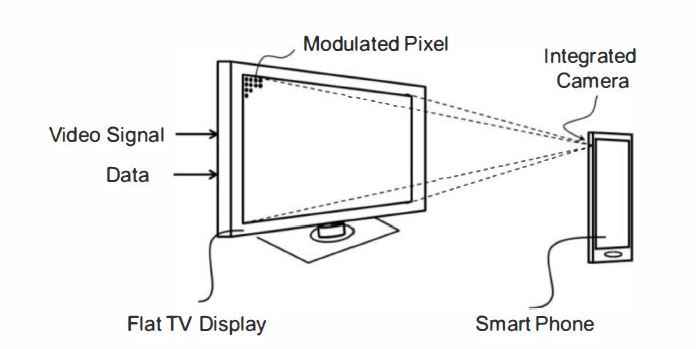
\includegraphics[keepaspectratio,width=0.8\textwidth]{images/David1.jpg}
 \caption{Eine beispielhafte Implementierung des DaViD-Systems}
 \label{fig:David1}
\end{figure}


\section{Systemmodell} 
Bild in Display enthalten eine große Anzahl von Pixeln, die jeweils aus einer spezifischen Anordnung von Subpixeln für die RGB-Farbraum bestehen. Jeder einzelne Frame des Videos wird nämlich durch eine Matrix von Subpixelwerten dargestellt. DaVid System verwendet eine differentielle Modulationsmethod d.h. Teil der Videoinformationen muss wiederholt werden, indem Daten als ein symmetrischer Manchester-Code moduliert und zu den Videosignalkomponenten hinzugefügt werden. In Empfängerseite durch eine zeitliche Synchronisation können die zeitliche \gls{ISI} vermieden werden. Dann nach Verwendung einer örtlichen Synchronisation enthalten einen Differenzbild. Weil die Randbereich des Differenzbilds ungültig ist, verlässt sich die Modulationsgebiet durch die Verfahren in diese Arbeit entdecken. Danach werden die überlagerten Datensequenz durch eine Reihe von Behandlungen vom Videoinhalt getrennt. Abbildung 2.2 zeigt die schematische Darstellung des DaVid-Systems. 
% Deshalb in zeitlicher oder örtlicher Richtung die Videoinhalt in paar Bildern werden gleich.
\vspace{18pt}

\begin{figure}[htb]
	\centering 
	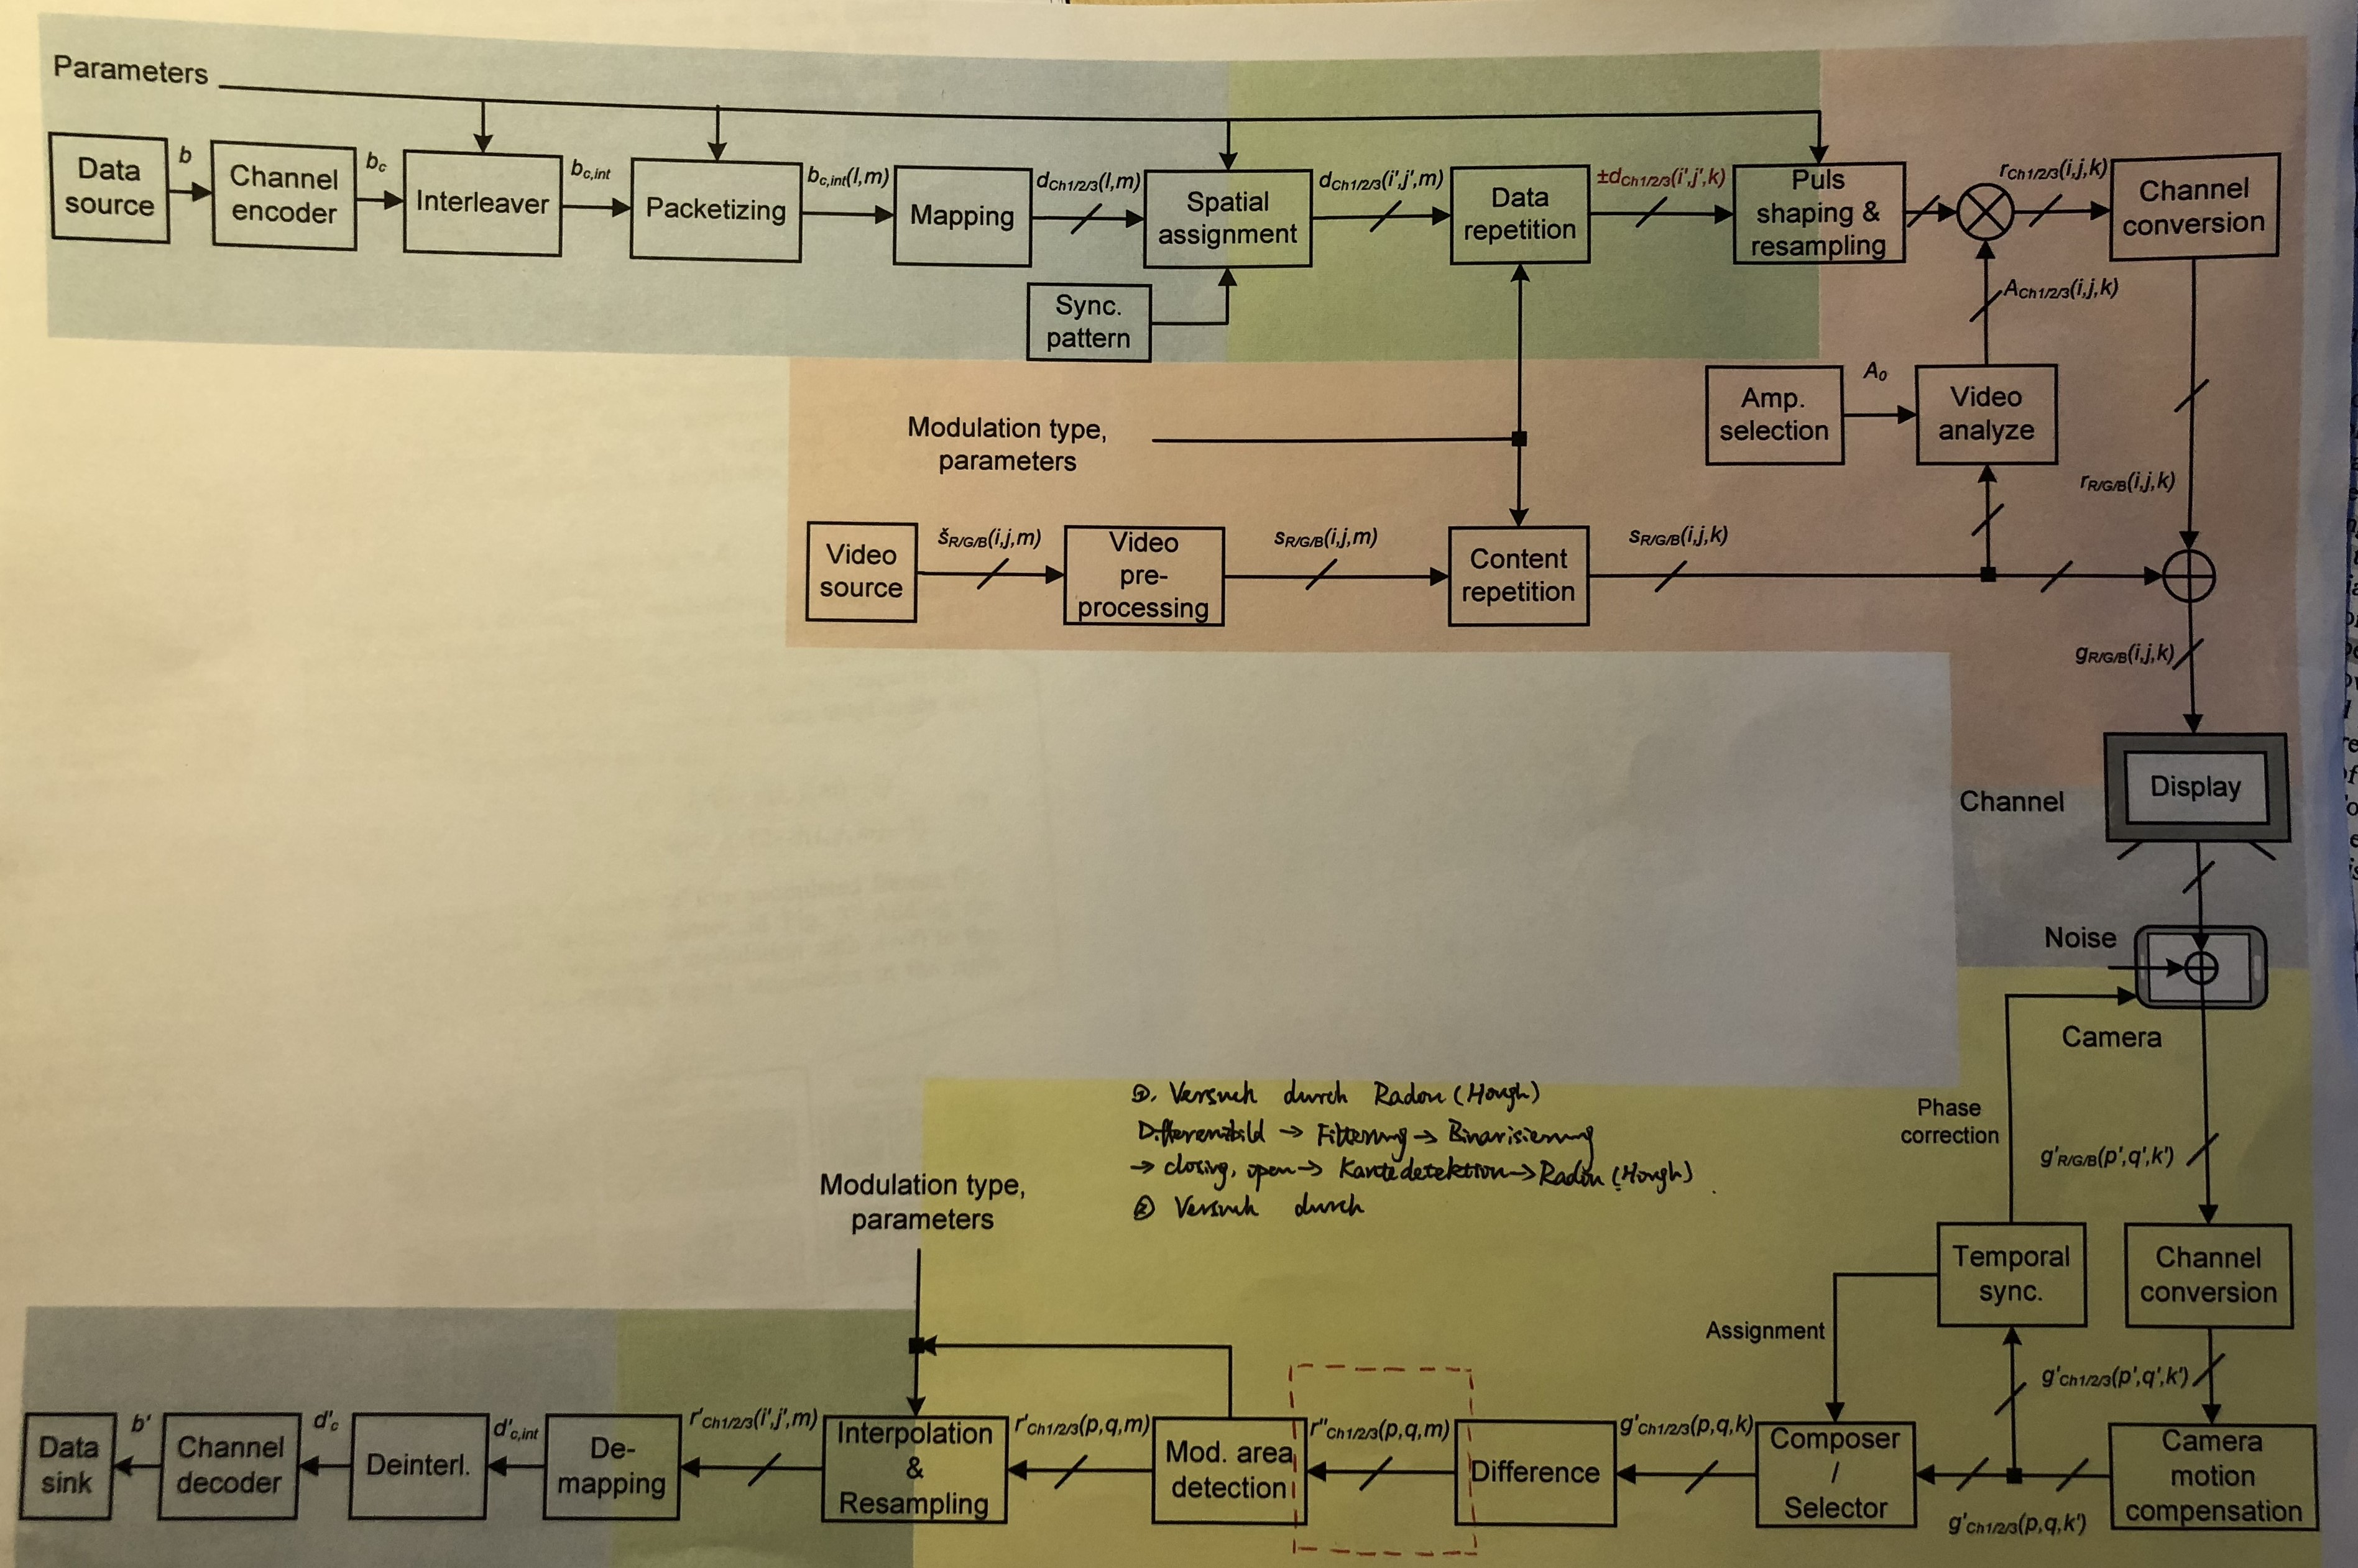
\includegraphics[keepaspectratio,width=1.0\textwidth]{images/David3.jpg}
	\caption{Schematische Darstellung von DaVid System}
	\label{fig:David2}
\end{figure}


\subsection{Modulationsverfahren}

Ein Modulationsverfahren, das die Videoqualität nicht offensichtlich reduziert garantiert, ist sehr wichtig für ein auf Videogerät basierendes Datenübertragungssystem. Die möglichen Modulationsverfahren in DaVid-System sind:
\begin{itemize}
	\item Zeitliche differentielle Modulation der Luminanz
	\item Zeitliche differentielle Modulation der Chrominanz
	\item Örtliche differentielle Modulation der Luminanz
	\item Örtliche differentielle Modulation der Chrominanz
\end{itemize}

Zeitliche differentielle Modulationsverfahre lässt kontinuierliches Paar Frames den gleichen Luminanz- bzw. Chrominanz-Videoinhalt enthalten, d.h. durch Subtrahieren die mit daten addiert Kanal der Paar Frames die Differenzbild erhalten lassen können. Dagegen in örtliche- sind die benachbarte Pixel mit den gleichen Videoamplituden. Im Vergleich zu Luminanzteil Y die Anzeigequalität in U und V Komponente ist signifikant besser, wenn Informationen in Chrominanz wiederholt und moduliert werden. Deswegen wird in dieser Arbeit nur zeitliche differentielle Modulation der Chrominanz verwendet. Abbildung 2.3 zeigt ein Blockdiagramm einer typischen Senderimplementierung durch zeitliche differentielle Modulation.

\begin{figure}[htb]
	\centering 
	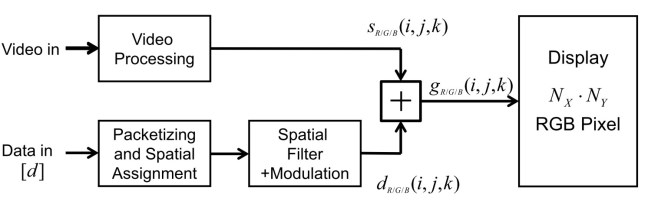
\includegraphics[keepaspectratio,width=0.8\textwidth]{images/David2.jpg}
	\caption{Blockschaltbild der Signalverarbeitung in zeitlicher differentieller Modulation}
	\label{fig:David3}
\end{figure}

Wir nehmen eine Diaplay an, die in horizontale Richtung $N_x$ Pixel stehen, dagegen in vertikale Richtung $N_y$ Pixel. Das Videoeingangssignal wird verarbeitet, um eine Anzeigeeingabe $s(i,j,k)$ zu liefern. Mit zeitliche differenziell Modulation ist die Videoinhalt des kommenden Frame dasselbe.Die Indizes i und j bedeuten die horizontale und vertikale Pixelposition auf dem Bildschirm, während k die Nummer des reproduzierten Bildes ist.
Indiz m heißt den Zähler des Frames in einer Videosequenz. Der Amplitudenbereich des Videosignals sollte begrenzt sein, um die Addition kleiner Datenamplituden ohne Übersteuern zu ermöglichen.

\begin{equation}
\begin{split}
 s_{R/G/B}&(i,j,k+1) = s(i,j,k) \\
          &  for \ 0\le i <N_x, 0\le j<N_y,k=2 \cdot m , m \in \mathbb{Z}\\
\end{split}
\end{equation}

Vor Datenübertragung muss der Datenstrom in Schichten der Länge L aufgeteilt werden. Indiz L bedeutet die Menge der Daten, die in einem Framepaar übertragen werden können. Ein direkter Ansatz ist eine direkte Zuordnung von Datenbits zu Pixeltripeln Zeile für Zeile.

\begin{equation}
\begin{split}
  & d(l)\rightarrow d(i,j,m) \qquad d(l)\in \{-1,1\} \\
  & 0\le l <L,L = N_x \cdot N_y \\
  & i=l \bmod N_x \qquad j=\lfloor l/N_x \rfloor \\
\end{split}
\end{equation}

Die Modulationsamplitude A ist ein wichtiger Parameter für Datenübertragung. Im Prinzip kann die Amplitude in verschieden Kanal unabhängig gewählt werden, um die Systemleistung zu optimieren. In diesen Arbeiten setzen die Amplitude gleichwertig.

\begin{equation}
 A_R=A_G=A_B=A        
\end{equation}

Das differentielle Modulationsverfahren ordnet jede Sequenz von $\left\{-A, A\right\}$ zu d = -1 bzw. $\left\{A, -A\right\}$ zu d = 1 zu. Modulierte Datensymbole und verarbeitete Videoamplituden werden addiert, um die Anzeigeeingabe $g(i,j,k)$ zu liefern:

\begin{equation}
\begin{split}
   s_{R/G/B}(i,j,k)  &= s_{R/G/B}(i,j,m) + A_{R/G/B} \cdot \left( 2 \cdot d(i,j,m) - 1 \right) \\
   s_{R/G/B}(i,j,k+1)&= s_{R/G/B}(i,j,m) - A_{R/G/B} \cdot \left( 2 \cdot d(i,j,m) - 1 \right) \\
\end{split}
\end{equation}

Ein Beispiel einer modulierten Bildfolge ist in Abbildung 2.4 gezeigt. Das Hinzufügen der modulierten Daten (hier mit A = 4) zu dem Videoeingang ergibt die Anzeigeamplituden in der rechten Spalte.
\newpage

\begin{figure}[htb]
	\centering 
	\includegraphics[keepaspectratio,width=0.8\textwidth]{images/David4.jpg}
	\caption{Ein Beispiel einer modulierten Bildfolge}
	\label{fig:David4}
\end{figure}


\begin{equation}
   T = \begin{pmatrix}
   0,213 & 0,715 & 0,072 \\
   -0,115& -0,385& 0,5	\\
   0,5   & -0,454& -0,0458
\end{pmatrix}  
\end{equation}


\begin{equation}
\begin{split}
  \begin{pmatrix}
  g_R(i,j,k) \\
  g_G(i,j,k) \\
  g_B(i,j,k) \\
\end{pmatrix} &= T^{-1} \cdot \left( T \cdot \begin{pmatrix}
  S_R(i,j,m) \\
  S_G(i,j,m) \\
  S_B(i,j,m) 
  \end{pmatrix}  + \begin{pmatrix}
  0 \\
  A_U \cdot d(i,j,m) \\
  A_V \cdot d(i,j,m) 
  \end{pmatrix} \right) \\  
  \begin{pmatrix}
  g_R(i,j,k+1) \\
  g_G(i,j,k+1) \\
  g_B(i,j,k+1) \\
\end{pmatrix} &= T^{-1} \cdot \left( T \cdot \begin{pmatrix}
  S_R(i,j,m) \\
  S_G(i,j,m) \\
  S_B(i,j,m) 
  \end{pmatrix}  - \begin{pmatrix}
  0 \\
  A_U \cdot d(i,j,m) \\
  A_V \cdot d(i,j,m) 
  \end{pmatrix} \right) \\ 
\end{split}
\end{equation}


\begin{equation}
   \begin{pmatrix}
   A_R \\
   A_G \\
   A_B
  \end{pmatrix}  = T^{-1} \cdot \begin{pmatrix}
   A_Y \\
   A_U \\
   A_V
  \end{pmatrix}
\end{equation}



\subsection{DatenBlock}

Um die Anforderungen an die Kameraauflösung zu lockern, Ein einfaches und unkompliziertes Verfahren ist Zuordnung jedes Datenbits zu einem Block von $B_X \times B_Y$ Pixeln.

\begin{equation}
\begin{split}
  & d(l)\rightarrow d(x,y,k) \qquad 0\le l <L \\
  & L=\lfloor N_X/B_X \rfloor \cdot \lfloor N_Y/B_Y \rfloor \\
  & x=(l \cdot B_X) \bmod N_X +r_X, \ r_X =0...(B_X -1) \\
  & y=\lfloor l / \lfloor N_X/B_X \rfloor \rfloor \cdot B_Y +r_Y, \ r_Y =0...(B_Y -1) \\
\end{split}
\end{equation}

Wenn die Anzahl der Pixel pro Zeile kein Vielfaches von $B_X$ ist oder wenn die Anzahl der Pixel kein Vielfaches von $B_Y$ ist, muss die Anzahl der Pixel und Zeilen, die für die Modulation in Gleichung $\left(2.5\right)$ verwendet werden, ersetzt werden durch:

\begin{equation}
\begin{split}
  & N_X = \lfloor N_X/B_X \rfloor \cdot B_X\\ 
  & N_Y = \lfloor N_Y/B_Y \rfloor \cdot B_Y\\ 
\end{split}
\end{equation}

% \newpage
In dieser Arbeit werden das DatenBlock für quadratische Blöcke gesetzt.

\begin{equation}
   B_X = B_Y = B.
\end{equation}





\section{Anwendungsgebiete} 
%\label{sec:Anwendungsbereiche}

Die Datenübertragungsrate des David-Systems wird voraussichtlich erreicht bis zu 100 Mbit/s. Es gehöre	zu einer Sichtlinienübertragung für kurze Verbindungen. Geeignete Abdeckungsbereichen hängen von der Größe des Displays und der Kameraoptik ab. Obwohl im Vergleich zum letzten WLAN- Versionen \gls{ieee} 802.11, die Leistung scheint nicht so attraktiv. Der Vorteil liegt nicht nur in der wachsenden Leistungsfähigkeit von Video-Display und Kamera, aber auch die Option zur Wiederverwendung der bestehenden Hardware, die zum Zeigen des Videos installiert wurde. Ein empfohlene praktische Anwendungsbereich des DaVids ist öffentlicher Ort, z.B. U-Bahn-Station, großes Stadion und so weiter. Annehmen eine Situation, wenn die Leute auf ihre U-Bahn warten, sie können ihre eigene Software aktualisieren, indem Sie einfach auf die zeigende Werbung in dem Bildschirm leiten.

Berücksichtigen der Eigenschaften des DaVids, d.h. die Synchronisation von Videospielen und Datenübertragung. Viele Anwendungsszenarien können in Betracht gezogen werden und scheinen sehr attraktiv zu sein. Die drei Hauptszenarien sind:

\begin{itemize}
  \item Indoor-individuelle Kommunikation: Kurzstreckenverbindungen basieren auf relativ kleinen (Tablet-Größe) Bildschirm, Anwendungen z.B. die Übertragung von Hintergrundinformationen an Besucher im Museum, Kiosk.
  \item Indoor-Multicast-Kommunikation:Streckabstand ist länger als ersten Fall auf relativ größer (40-100") Bildschirm, Anwendungen z.B. während Videoabspielen Besucher die Anwendungsdaten oder Mediendateien herunterladen können im Kiosk, Restaurant.
  \item Freien Kommunikation: Größter Bildschirm wie im Einkaufszentren oder Sport-Arenen, Anwendungen können denen des zweiten Szenarios ähneln.
\end{itemize}

Sobald die Dienste auf öffentlichen Bildschirmen implementiert werden, kann Leute mit Hilfe eines modernen Smartphones, die mit einer geeigneten Kamera eingebaut ist, nach der Installation einer neuen App innovative wahrnehmen.






















\chapter{Untersuchung vom ersten Verfahren mittels Mustererkennung } 

In diesem Kapitel wird auf die Realisierung des ersten Verfahrens eingegangen. Zuerst wird die Bildregistrierung im Detail besprochen. Anschließend läuft die Differenzbild Optimierung und die benötigte Bildverarbeitung. Schließlich wird die QR Mustererkennung erläutert. Zur Implementierung dieses Verfahrens wird Matlab unter der Lizenz der TU Dortmund verwendet.

\section{Allgemeine Struktur} 

Dieses Verfahren verwendet die Charakteristiken der Datenmodulation des \gls{david} Systems, d.h. an jeder Ecke der Datenebene wird ein QR Muster hinzugefügt und dann zusammen mit den Daten hinter dem Bild moduliert. Am Empfänger wird nach einigen Operationen das QR Muster mit den in diesem Kapitel vorgestellten Verfahren detektiert und schließlich der Modulationsbereich bestimmt. Diese Methode löst den unansehnlichen Effekt, dass das QR Muster direkt zum Bild hinzugefügt wird. Außerdem wird die Detektion mit der QR-Mustereigenschaft günstig und effektiv implementiert. Abbildung \ref{fig:Strukturdiagramm} zeigt das Strukturdiagramm dieses Verfahrens.

\begin{figure}[H]
 \centering 
 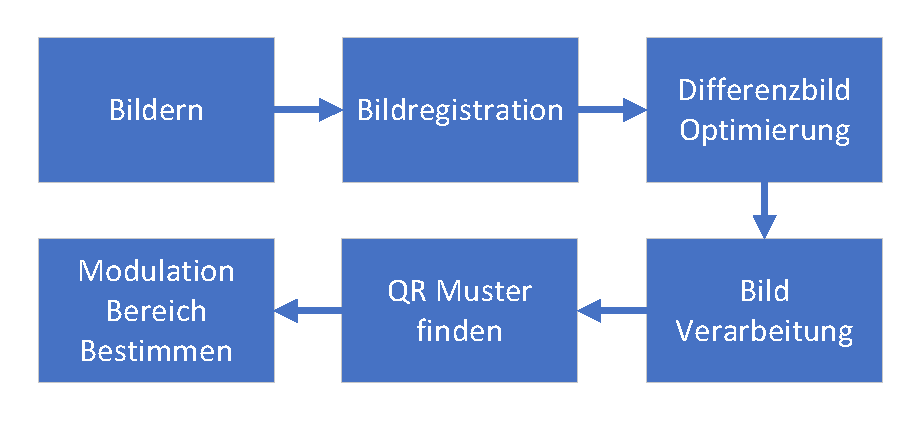
\includegraphics[keepaspectratio,width=1.0\textwidth]{images/3_Ersteverfahren/Strukturdiagramm.pdf}
 \caption{Strukturdiagramm}
 \label{fig:Strukturdiagramm}
\end{figure}

Das Objekt, das mit dieser Methode bearbeitet wird, ist eine aus einer spezifischen Smartphone App $ ``VLCReceiver" $ gesammelte Bilderreihe. Diese App wurde speziell für das \gls{david}-System entwickelt und erstellt eine Reihe von Bildern bei jeder Aufnahme. Im Allgemeinen wird die Kamera bei der Aufnahme in der Hand gehalten. Aufgrund von Handschütteln während der Aufnahme entsteht eine leichte Verschiebung zwischen den Bildern. Um dieses Problem zu beheben, wird eine Bildregistrierungsoperation verwendet, die zwei Bilder einer Aufnahme in dasselbe Koordinatensystem konvertiert. Zuerst werden durch \gls{surf} Merkmalserkennung Merkmale der Bilder verglichen. 
Durch Merkmalsextraktion und Merkmalsanpassung werden die Korrespondenzpunkte zwischen den verglichenen Bildern erhalten. Der \gls{ransac} Algorithmus benötigt, um die irrelevanten Korrespondentenpunkte zu beseitigen und die Genauigkeit zu verbessern. Aus dem Kameramodell wird anschließend ein mathematisches Transformationsmodell zwischen den entsprechenden Punkten in den beiden Bildern erstellt. Es ist zu beachten, dass der Prozess zur Lösung des Transformationsmodells als ein nichtlineares Optimierungsproblem angesehen werden kann. Durch die Lösung dieses Problems kann die Transformationsmatrix erhalten werden. In dieser Arbeit wird immer das erste Bild als Referenzbild gewählt um eine Bildregistrierung mit folgenden Bildern vorzunehmen. Die von der Bildregistrierung enthaltenen Bilder werden in dasselbe Koordinatensystem umgewandelt. Es werden je zwei Bilder subtrahiert, wodurch eine Reihe Differenzbilder entstehen. Um die folgende Detektion zu vereinfachen, wird eine Optimierungsoperation mit der Hilfe der geometrischen Eigenschaft des QR Musters unternommen woraufhin ein zu detektierendes Bild erstellt wird. Anschließend werden eine Reihe von Bildverarbeitungen bzw. Binarisierung, Medianfilter, Morphologie Operation vorgenommen. Dadurch können vereinzelt Punkte und Lücken, die durch Rauschen und Fehler verursacht wurden, entfernt werden. Schließlich wird es durch die Charakteristik des QR Musters, dessen Breiteverhältnis $1:1:3:1:1$ beträgt um QR Muster zu detektieren. Dies bestimmt auch den Modulationsbereich. Das Flussdiagramm wird in Abbildung \ref{fig:Flussdiagramm der Methode} gezeigt. Die Details jedes Teils werden in den folgenden Abschnitten beschrieben.

\begin{figure}[H]
 \centering 
 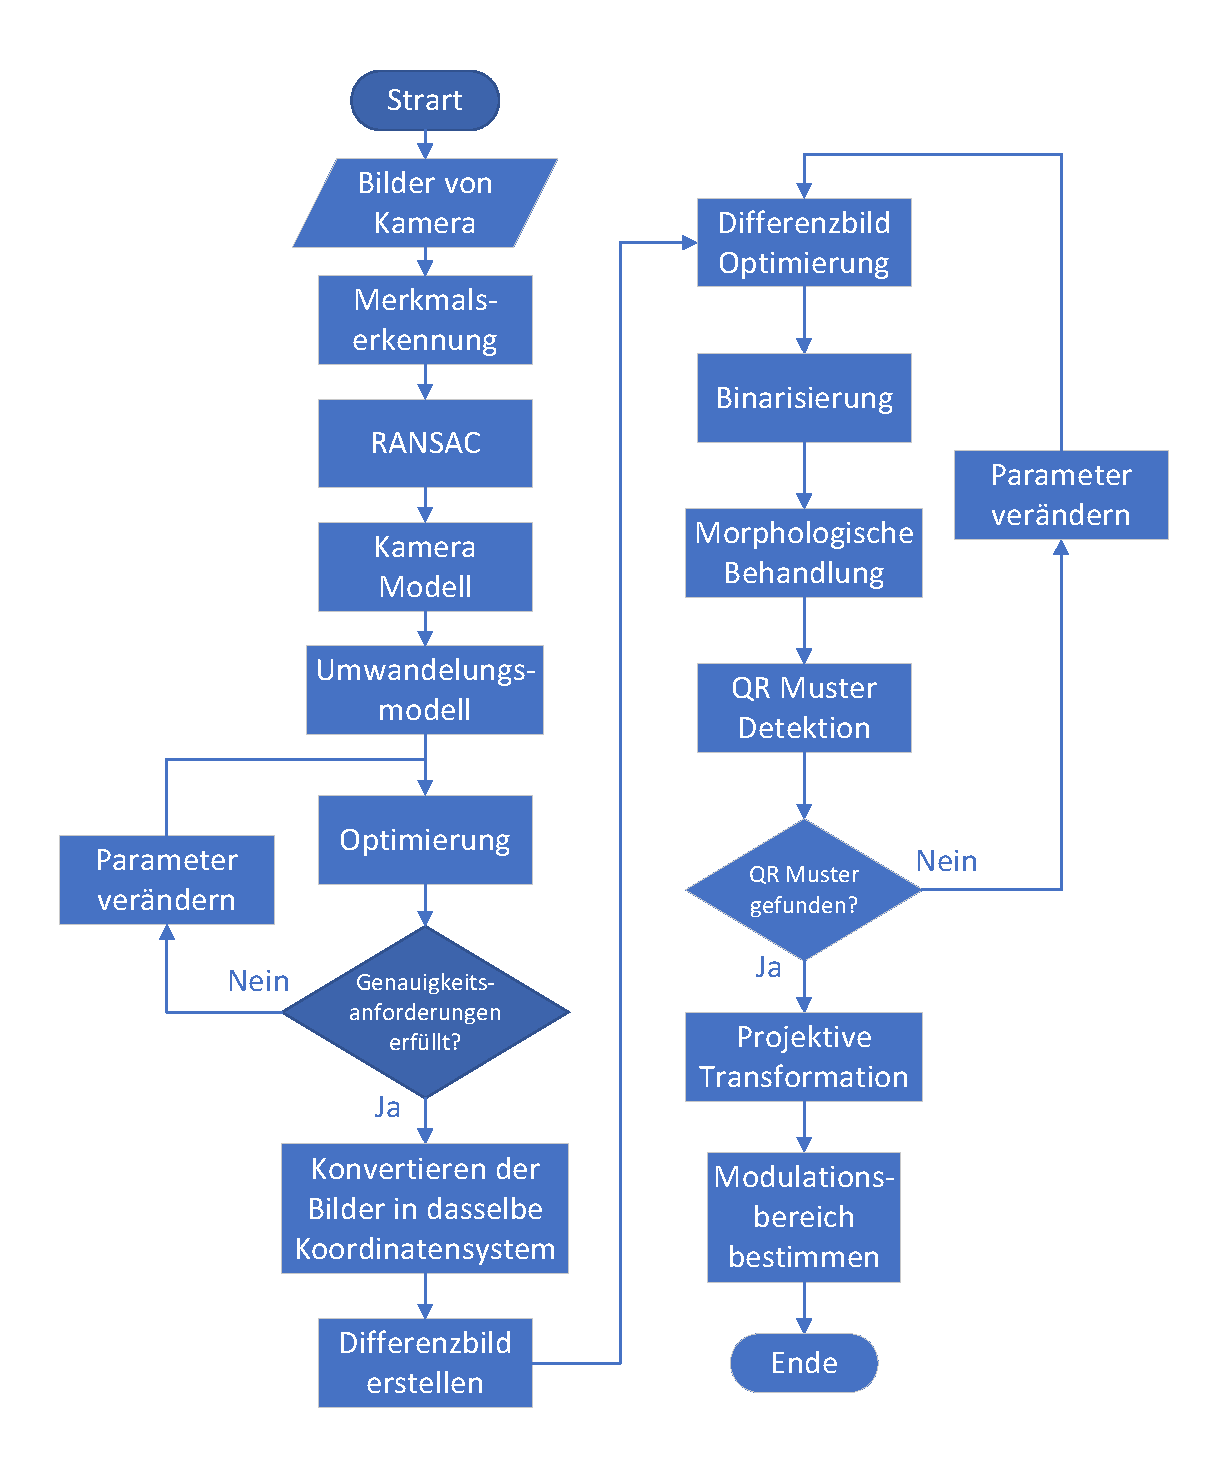
\includegraphics[keepaspectratio,width=1.0\textwidth]{images/3_Ersteverfahren/Flussdiagrammsum.pdf}
 \caption{Flussdiagramm der ersten Methode}
 \label{fig:Flussdiagramm der Methode}
\end{figure}

\section{Bildregistrierung} 

Es wird angenommen, eine Reihe Bilder wird mit einer Handheld-Kamera aufgenommen. Es kommt aufgrund von Handbewegungen zu einer leichten Verschiebung zwischen den beiden benachbarten Bildern. Wenn diese Bilder subtrahiert werden, um die Differenzbilder zu erhalten, wird das Ergebnis sehr schlecht sein. Um dieses Problem zu lösen, wird hier Bildregistrierung eingeführt. Ein Flussdiagramm der Bildregistrierung wird in Abbildung 4.2 gezeigt. 

\begin{figure}[H]
 \centering 
 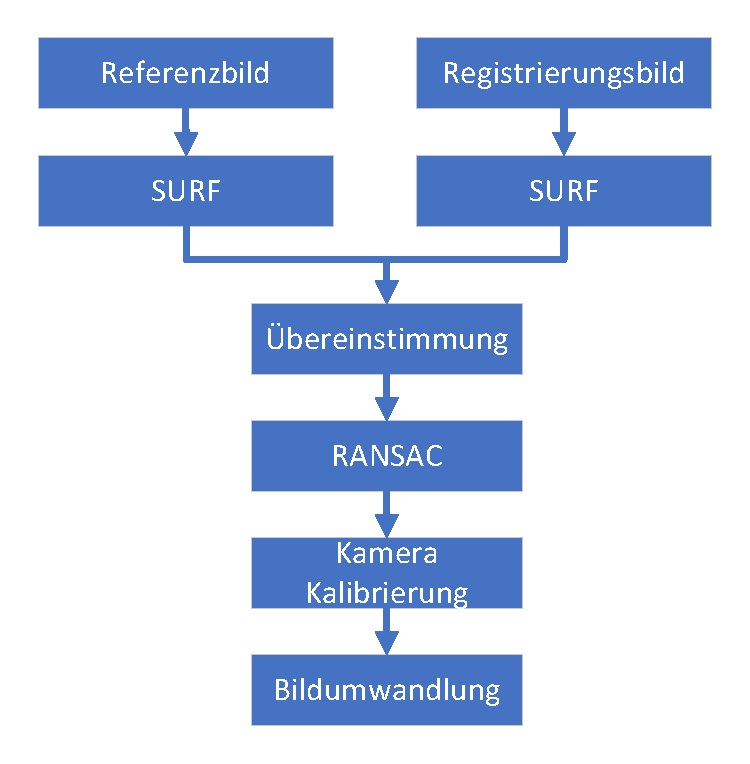
\includegraphics[keepaspectratio,width=0.6\textwidth]{images/3_Ersteverfahren/Bildregistration.pdf}
 \caption{Flussdiagramm der Bildregistrierung}
 \label{fig:Bildregistrierung}
\end{figure}

\subsection{\gls{surf}}
In jedem Bild gibt es eindeutige Pixelwertpunkte, d.h. Merkmalspunkte des Bildes. Um die Bilder in dasselbe Koordinatensystem zu transformieren, müssen diese Merkmalspunkte erkannt und analysiert werden. Deswegen ist es in diesem Verfahren besonders wichtig, die Merkmalspunkte eines Bildes zu definieren und zu finden. Um dieses Problem zu lösen, wird das Konzept der Merkmalserkennung eingeführt. Diese wird oft in Computer Vision und Bildverarbeitungsbereichen verwendet. Die Merkmalserkennung beinhaltet Verfahren zum Berechnen von Abstraktionen von Bildinformationen und zum Treffen lokaler Entscheidungen an jedem Bildpunkt, ob es an einem Punkt ein Bildmerkmal eines bestimmten Typs gibt oder nicht. Einige typische Merkmalserkennungen sind z.B. Kantenerkennung, Eckenerkennung, Tropfenerkennung und so weiter.

In dieser Arbeit wird das \gls{surf} \cite{Surf} genutzt. 
Dieser ist ein patentierter lokaler Merkmal-Detektor und Deskriptor und kann für Aufgaben wie Objekterkennung, Bildregistrierung, Klassifizierung oder 3D-Rekonstruktion angewandt werden. Diese Merkmalserkennung ist eine verbesserte Version von \gls{sift} Merkmalserkennung, die Haar-Wavelet verwendet um die Gradientenoperation in der \gls{sift}-Methode zu ersetzen, und gleichzeitig eine Integralgraph-Technik für schnelle Berechnungen verwendet. Die Faltung bezieht sich nur auf das vorherige Bild. Durch die Vergrößerung des Bildkerns kann das Heruntertaktungsverfahren realisiert werden. Die Geschwindigkeit von \gls{surf} ist 3-7 mal schneller als die von \gls{sift} welche in den meisten Fällen der Leistung von \gls{sift} entspricht. Daher wird \gls{surf} in vielen Anwendungen eingesetzt, insbesondere in Anwendungen in denen die Laufzeitanforderungen hoch sind. 

Der Verlauf einer \gls{surf} Merkmalserkennung ist wie folgend:

$\bullet$ \textbf{Aufbau einer hessischen Matrix.}\\
Die Hesse-Matrix stellt den Kern des \gls{surf} Algorithmus dar. Zur Vereinfachung der Operation wird für die Funktion $f(x,y)$ angenommen, dass sich die Hesse-Matrix H aus partiellen Ableitungen und Funktionen zusammensetzt.

\begin{equation}
   H(f(x,y)) = \begin{bmatrix}
   \frac{\partial^{2}f}{\partial x^{2}} & \frac{\partial^{2}f}{\partial x \cdot \partial y} \\
   \frac{\partial^{2}f}{\partial x \cdot \partial y} & \frac{\partial^{2}f}{\partial y^{2}} \\   
   \end{bmatrix}
\end{equation}

 Determinante der H-Matrix ist wie folgt:
 
\begin{equation}
   \det(H) = \frac{\partial^{2}f}{\partial x^{2}} \cdot \frac{\partial^{2}f}{\partial y^{2}} - (\frac{\partial^{2}f}{\partial x \cdot \partial y})^2  
\end{equation}

Der Wert der Determinante ist der Eigenwert der H-Matrix. Durch dessen positiven und negativen Wert wird bestimmt, ob der Punkt ein Extrempunkt ist oder nicht. Im \gls{surf} Algorithmus wird das Bildpixel $l(x,y)$ anstelle des Funktionswertes $f(x,y)$ verwendet. Es wird eine Gauß-Funktion zweiter Ordnung als Filter verwendet. Die zweiten partiellen Ableitungen können durch Faltung zwischen bestimmten Kernen berechnet werden. Dadurch können die Werte der drei Matrixelemente der H-Matrix ebenfalls berechnet werden.

\begin{equation}
\begin{split}
   &\mathcal{H}(\textbf{x},\sigma) = \begin{bmatrix}
   L_{xx}(\textbf{x},\sigma)\ L_{xy}(\textbf{x},\sigma) \\
   L_{xy}(\textbf{x},\sigma)\ L_{yy}(\textbf{x},\sigma)
   \end{bmatrix} \\   
   &L(\textbf{x},\sigma) = G(\sigma)*I(\textbf{x}) \\  
   &G(\sigma) = \frac{\partial^{2}g(\sigma)}{\partial x^{2}}      
\end{split}
\end{equation}


Hier bedeutet $L_{xx}(\textbf{x},\sigma)$ die Faltung der zweiten Gaußschen Ableitung $G(\sigma)$ mit dem Bild I im Punkt $\textbf{x}$(x,y), das selbe für $L_{xy}(\textbf{x},\sigma)$ und $L_{yy}(\textbf{x},\sigma)$. Auf diese Weise kann der Wert der Determinante für jedes Pixel in dem Bild berechnet werden und dieser Wert kann verwendet werden um den Merkmalspunkt festzustellen.
Zur einfacheren Anwendung schlägt Herbert Bay\cite{Surf} vor, L mit einer Approximation zu ersetzen. Um den Fehler zwischen dem genauen Wert und der Approximation auszugleichen, kann die H-Matrix-Determinante wie folgt ausgedrückt werden:

\begin{equation}
   \det(\mathcal{H}_{Approx}) = D_{xx}D_{yy} - (0.9D_{xy})^2  
\end{equation}
\\
$\bullet$ \textbf{Erstellen des Maßstabraums}\\
Der Maßstabraum $L(\textbf{x},\sigma)$ des Bildes ist die Darstellung dieses Bildes bei unterschiedlichen Auflösungen(Skalierungen). Im Bereich der Computer Vision wird der Maßstabraum symbolisch als Bildpyramide ausgedrückt, wobei die Eingangsbildfunktion wiederholt mit dem Kern der Gaußschen Funktion gefaltet und wiederholt unterabgetastet wird. Diese Methode wird hauptsächlich für die Implementierung des \gls{sift} Algorithmus verwendet. Jede Bildschicht hängt jedoch von der vorherigen Bildschicht ab, weshalb das Bild in der Größe angepasst werden muss. Daher büßt diese Berechnungsmethode viel Leistung ein. Das Gegenstück in \gls{surf} ist die Erhöhung der Größe des Bildkerns. Dies ist ein Unterschied zwischen dem \gls{sift} Algorithmus und dem \gls{surf} Algorithmus bei der Verwendung des Pyramidenprinzips.
Der Algorithmus ermöglicht, dass mehrere Bilder des Maßstabraums gleichzeitig verarbeitet werden, ohne dass das Bild unterabgetastet wird, wodurch die Leistung des Algorithmus verbessert wird. Das linke Bild in Abbildung \ref{fig:Scale space} ist eine Pyramidenstruktur, die auf herkömmliche Weise erstellt wird. Die Größe des Bildes wird geändert, und die Operation wird die Unterebene  unter Verwendung der Gaußschen Funktion wiederholt glätten. Der \gls{surf} Algorithmus auf der rechten Seite in Abbildung \ref{fig:Scale space} erhält das ursprüngliche Bild und ändert nur die Filtergröße.

\begin{figure}[htb]
 \centering 
 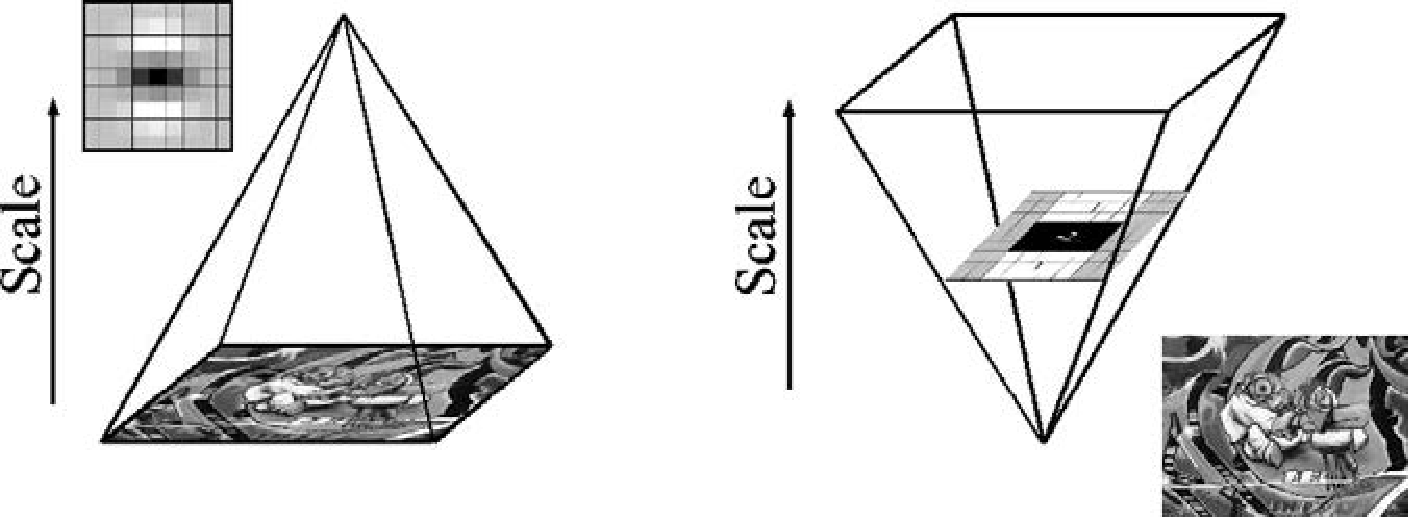
\includegraphics[keepaspectratio,width=0.8\textwidth]{images/3_Ersteverfahren/Scale_space.pdf}
 \caption{Scale space}
 \label{fig:Scale space}
\end{figure} 


$\bullet$ \textbf{Präzise Lokalisierung von Feature-Punkten}\\
Die von der Hesse-Matrix verarbeitete Größe jedes Pixels wird mit den 26 Punkten der drei Dimensionen im Raum, wie in Abbildung \ref{fig:Extremwert Erkennung} gezeigt, verglichen. Wenn einer davon das Maximum oder Minimum dieser 26 Punkte ist, wird dieser als vorläufiger Merkmalspunkt beibehalten. Das dreidimensionale lineare Interpolationsverfahren wird angewandt, um die Merkmalspunkte des Subpixel-Niveaus zu erhalten. Die Punkte, deren Werte kleiner als ein bestimmter Schwellenwert sind, werden ebenfalls entfernt.

\begin{figure}[htb]
 \centering 
 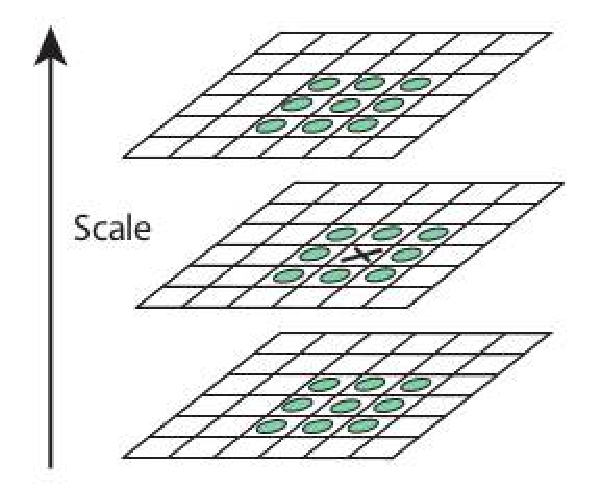
\includegraphics[keepaspectratio,width=0.4\textwidth]{images/3_Ersteverfahren/Extreme_Wert_Erkennung.pdf}
 \caption{Extremwert Erkennung}
 \label{fig:Extremwert Erkennung}
\end{figure} 


$\bullet$ \textbf{Hauptrichtungsermittlung}\\
\gls{sift} wählt die Hauptrichtung des Merkmalspunkts unter Verwendung des Gradientenhistogramms im Merkmalspunktbereich aus. Die Richtung, darin der Bin-Wert des Histogramms der größte ist oder 80\% des maximalen Bin-Werts überschreitet, wird als Hauptrichtung des Merkmalspunkts genommen. Dagegen beim \gls{surf}, wird nicht das Gradientenhistogramm, sondern die Haar-Wavelet-Eigenshcaft im Merkmalspunktbereich statistisch analysiert. Das heißt, im Bereich der Merkmalspunkte wird (zum Beispiel innerhalb eines Kreises mit einem Radius von 6\si{s}, wobei s der Maßstab ist auf dem der Punkt liegt), die Summe der Horizontal-Haar-Wavelet-Merkmale und der Vertikal-Haar-Wavelet-Merkmale aller Punkte im  60-Grad-Sektor($\pi/3$) gezählt. Die Größe des Haar-Wavelets beträgt 4\si{s}, sodass jeder Sektor einen Wert bekommt. Anschließend wird der 60-Grad-Sektor in einem bestimmten Intervall gedreht. Schließlich lässt die Richtung des Sektors anhand des Maximalwerts als Hauptrichtung vom Merkmalspunkt nehmen. Ein schematisches Diagramm des Prozesses ist wie folgt in Abbildung \ref{fig:Dominante Orientierung Feststellen}.

\begin{figure}[htb]
 \centering 
 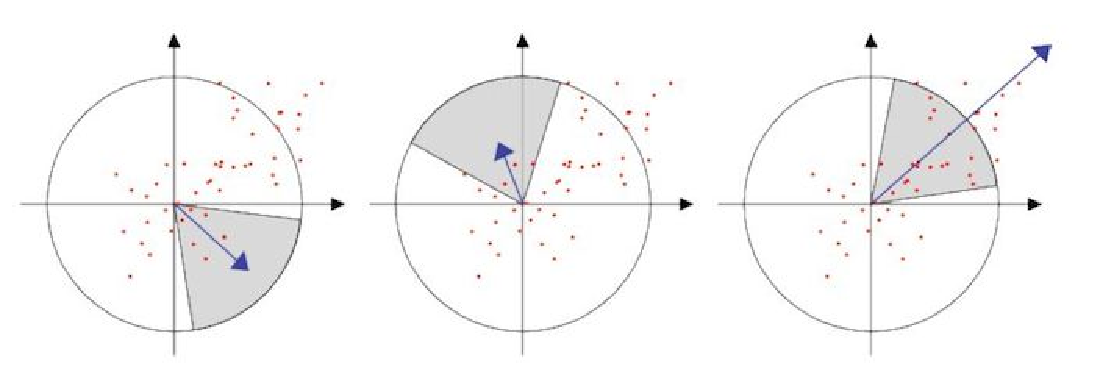
\includegraphics[keepaspectratio,width=0.8\textwidth]{images/3_Ersteverfahren/Dominante_Orientierung_Feststellen.pdf}
 \caption{Dominante Orientierung feststellen}
 \label{fig:Dominante Orientierung Feststellen}
\end{figure} 


$\bullet$ \textbf{Merkmalspunkt Deskriptor Generierung}\\
\gls{surf} generiert einen quadratischen Rahmen um den Merkmalspunkt. Die Größe der Seite des Rahmens ist 20\si{s} (s ist die Skala, dabei ein Merkmalspunkt erkannt wird). Die Richtung des Rahmens ist die Hauptrichtung, die im vorherigen Schritt erfasst wurde. Der Rahmen wird dann in 16 Unterbereiche unterteilt, von denen jeder die Haar-Wavelet-Merkmale der horizontalen und vertikalen Richtungen von 25 Pixeln berechnet. Hier sind die horizontalen und vertikalen Richtungen relativ zur Hauptrichtung. Das Haar-Wavelet-Merkmal ist die Summe der horizontalen Richtungswerte, die Summe der absoluten Werte in der horizontalen Richtung, die Summe der vertikalen Richtungen und die Summe der absoluten Werte in der vertikalen Richtung. Das schematische Diagramm in Abbildung \ref{fig:Merkmalspunkt Deskriptor} zeigt diesen Prozess.

\begin{figure}[htb]
 \centering 
 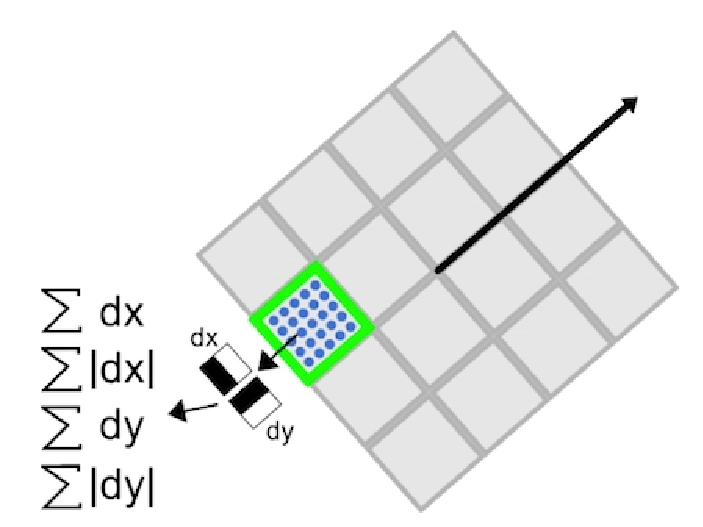
\includegraphics[keepaspectratio,width=0.5\textwidth]{images/3_Ersteverfahren/Merkmalspunkt_Deskriptor.pdf}
 \caption{Merkmalspunkt Deskriptor}
 \label{fig:Merkmalspunkt Deskriptor}
\end{figure} 

Auf diese Weise hat jeder kleine Bereich 4 Werte, so dass jeder Merkmalspunkt über einen $16*4=64$ dimensionalen Vektor verfügt, der nur halb so groß wie \gls{sift}(128 Dimension) ist, und deshalb den Anpassungsprozess beim Merkmalanpassungsprozess stark beschleunigt. Die folgende Abbildung \ref{fig:SURF Merkmal} zeigt die Merkmalspunkte, die durch den \gls{surf}-Algorithmus erhalten werden.

\begin{figure}[H]
 \centering 
 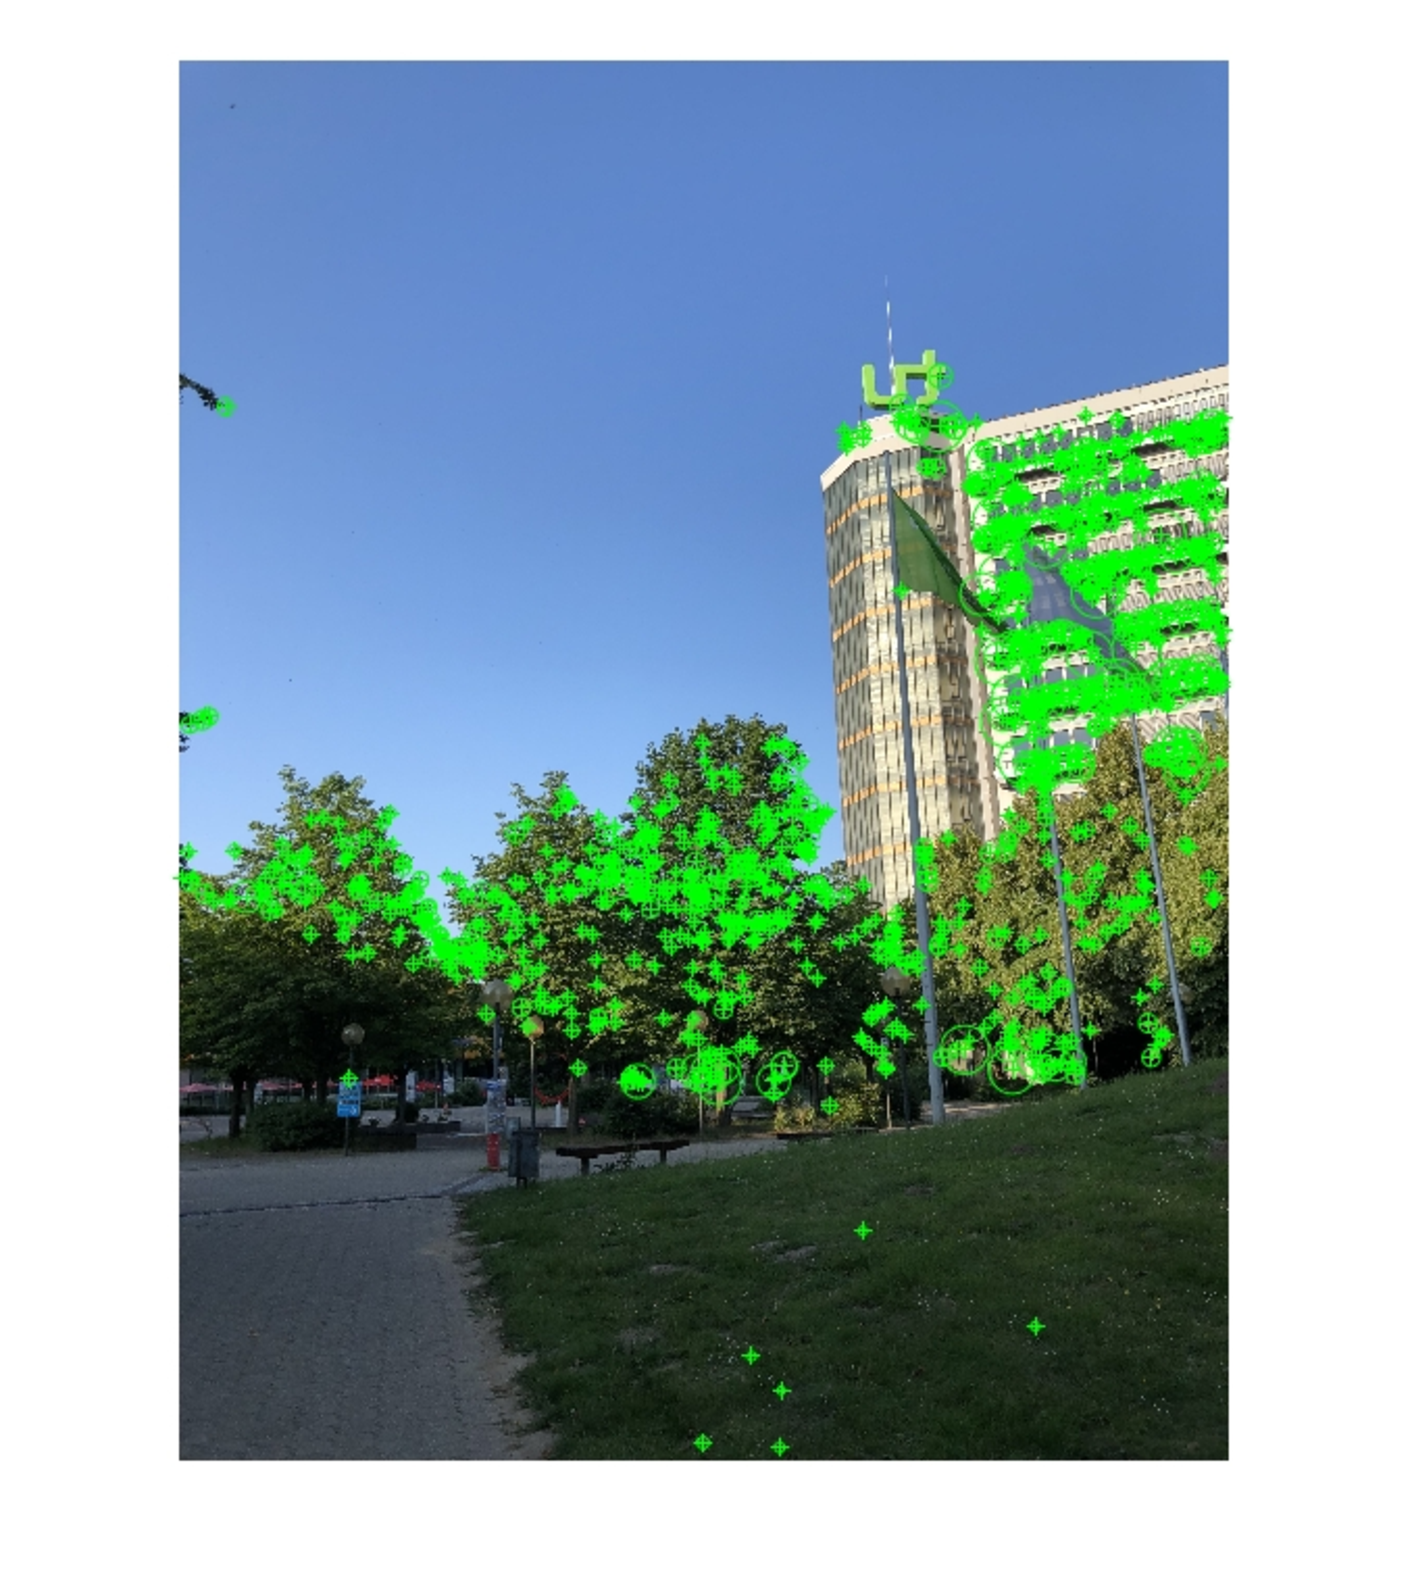
\includegraphics[keepaspectratio,width=0.8\textwidth]{images/3_Ersteverfahren/SURF_Detektion.pdf}
 \caption{\gls{surf} Merkmale}
 \label{fig:SURF Merkmal}
\end{figure} 


\subsection{\gls{ransac}}

Nach der \gls{surf} Merkmalserkennung werden die Merkmale von zwei benachbarten Bildern generiert. Diese Merkmale werden dann extrahiert und abgeglichen um entsprechende Punkte in den benachbarten zwei Bildern zu erhalten. Leider verbleiben durch diese Operation immernoch viele fehlerhafte zusammenpassende Paare. Deswegen wird hier \gls{ransac} verwendet, um die falschen Punkte zu beseitigen.

Der im Jahre 1981 vorgestellte \gls{ransac} Algorithmus von Fischler und Bolles \cite{ransac1}, ist ein allgemeiner Parameterschätzungsansatz um den großen Anteil von Ausreißern in den Eingabedaten zu bewältigen. Im Gegensatz zu vielen der üblichen robusten Schätzverfahren wie M-Schätzer und kleinste Quadrate, die von der Computer Vision Community aus der Statistik-Literatur übernommen wurden, wurde \gls{ransac} von der Computer-Vision-Community entwickelt. 

Ein einfaches Beispiel ist in der Abbildung \ref{fig:Linien Detektion} dargestellt. Das Ziel besteht darin, die am besten geeignete Linie unter einer Menge von Datenpunkten zu finden. Wenn es die einfache Methode der kleinsten Quadrate verwendet um diese Linie zu finden, wie auf der linken Seite gezeigt, kann es leider nicht richtig funktionieren, da die Methode der kleinsten Quadrate von allen Datenpunkten beeinflusst wird. Dagegen kann mit \gls{ransac} das Modell nur mit Potenziell korrekten Punkten berechnet werden, wie die Ergebnisse auf der rechten Seite zeigen. 

\begin{figure}[H]
 \centering 
 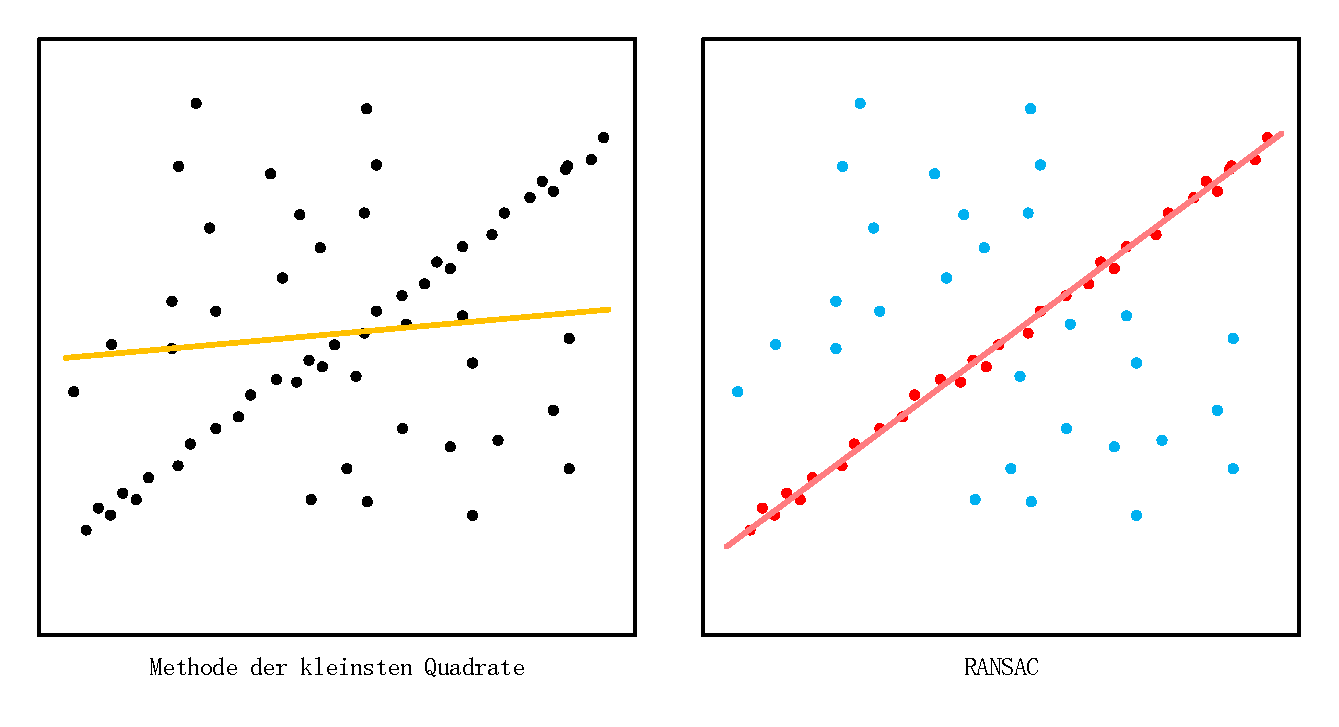
\includegraphics[keepaspectratio,width=1.0\textwidth]{images/3_Ersteverfahren/RANSAC/Linien_Detektion.pdf}
 \caption{Linien Detektion}
 \label{fig:Linien Detektion}
\end{figure} 

\gls{ransac} ist ein Wiederholungsprobennahme-Verfahren, welches durch die minimale Anzahl von Beobachtungenpunkten (Datenpunkten) die Kandidatenlösung generiert. Diese Datenpunkte sind erforderlich, um die zugrundeliegenden Modellparameter zu schätzen worauf Fischler und Bolles~\cite{ransac1} hingewiesen haben. Die Erhaltung einer anfänglichen Lösung und Ausschließung der Ausreißer mit dem \gls{ransac} Verfahren benötigt nicht so viele Daten, sondern verwendet die kleinste mögliche Menge und fährt fort, diese Menge mit konsistenten Datenpunkten zu vergrößern.

Der grundlegende Algorithmus ist wie folgt zusammengesetzt:

\begin{itemize}
	\item Zufällige Auswahl der Mindestanzahl erforderlicher Punkte zum Bestimmen der Modellparameter.
	\item Lösen der Parameter des Modells.
	\item Bestimmung der Punkte aus der Menge aller Punkte, welche mit einer vordefinierten Toleranz $\epsilon$ übereinstimmen
	\item Wenn ein Bruchteil der Anzahl von Inlierern über die Gesamtzahl der Punkte in dem Satz einen vordefinierten Schwellenwert $\tau$ überschreitet, schätzen die Modellparameter mit allen identifizierten Inlierern und terminieren.
	\item Ansonsten Wiederholung der Schritte 1 bis 4 (maximal N-mal).
\end{itemize}

N ist die Anzahl der Iterationen. Diese wird hoch genug gewählt, um die Wahrscheinlichkeit p (normalerweise 0.99) sicherzustellen, dass mindestens eine der Gruppen von Stichproben keinen Ausreißer enthält. Die Wahrscheinlichkeit, dass bei N mal iterieren mit erforderlich minimaler Anzahl von Punkten (hier m annahmen) mindestens ein Ausreißer mit ausgewählt wird, berechnet sich folgendermaßen:

\begin{equation}
   1 - p = (1 - u^m)^N
\end{equation}

u stellt die Wahrscheinlichkeit dar, dass jeder ausgewählte Datenpunkt ein Inlierer ist. Dagegen ist $v=1-u$ die Wahrscheinlichkeit, dass jeder ausgewählte Datenpunkt ein Ausreißer ist. Durch einige Gleichheitsumwandlungen kann die Anzahl der Iterationen ausgedrückt werden als:

\begin{equation}
   N = \frac{\log(1 - p)}{\log(1 - (1 - v)^m)}
\end{equation}

Abbildung \ref{fig:OhneRANSAC} zeigt die passenden Punkte durch Merkmalübereinstimmung mit der \gls{surf} Detektion. Es ist ersichtlich, dass es viele fehlerhafte Kombinationen gibt. Durch die Anwendung von \gls{ransac} kann dieses Problem effektiv gelöst und die übereinstimmenden Punkte verfeinert werden, wie das Ergebnis in Abbildung \ref{fig:MitRANSAC} zeigt.

\begin{figure}[H]
 \centering 
 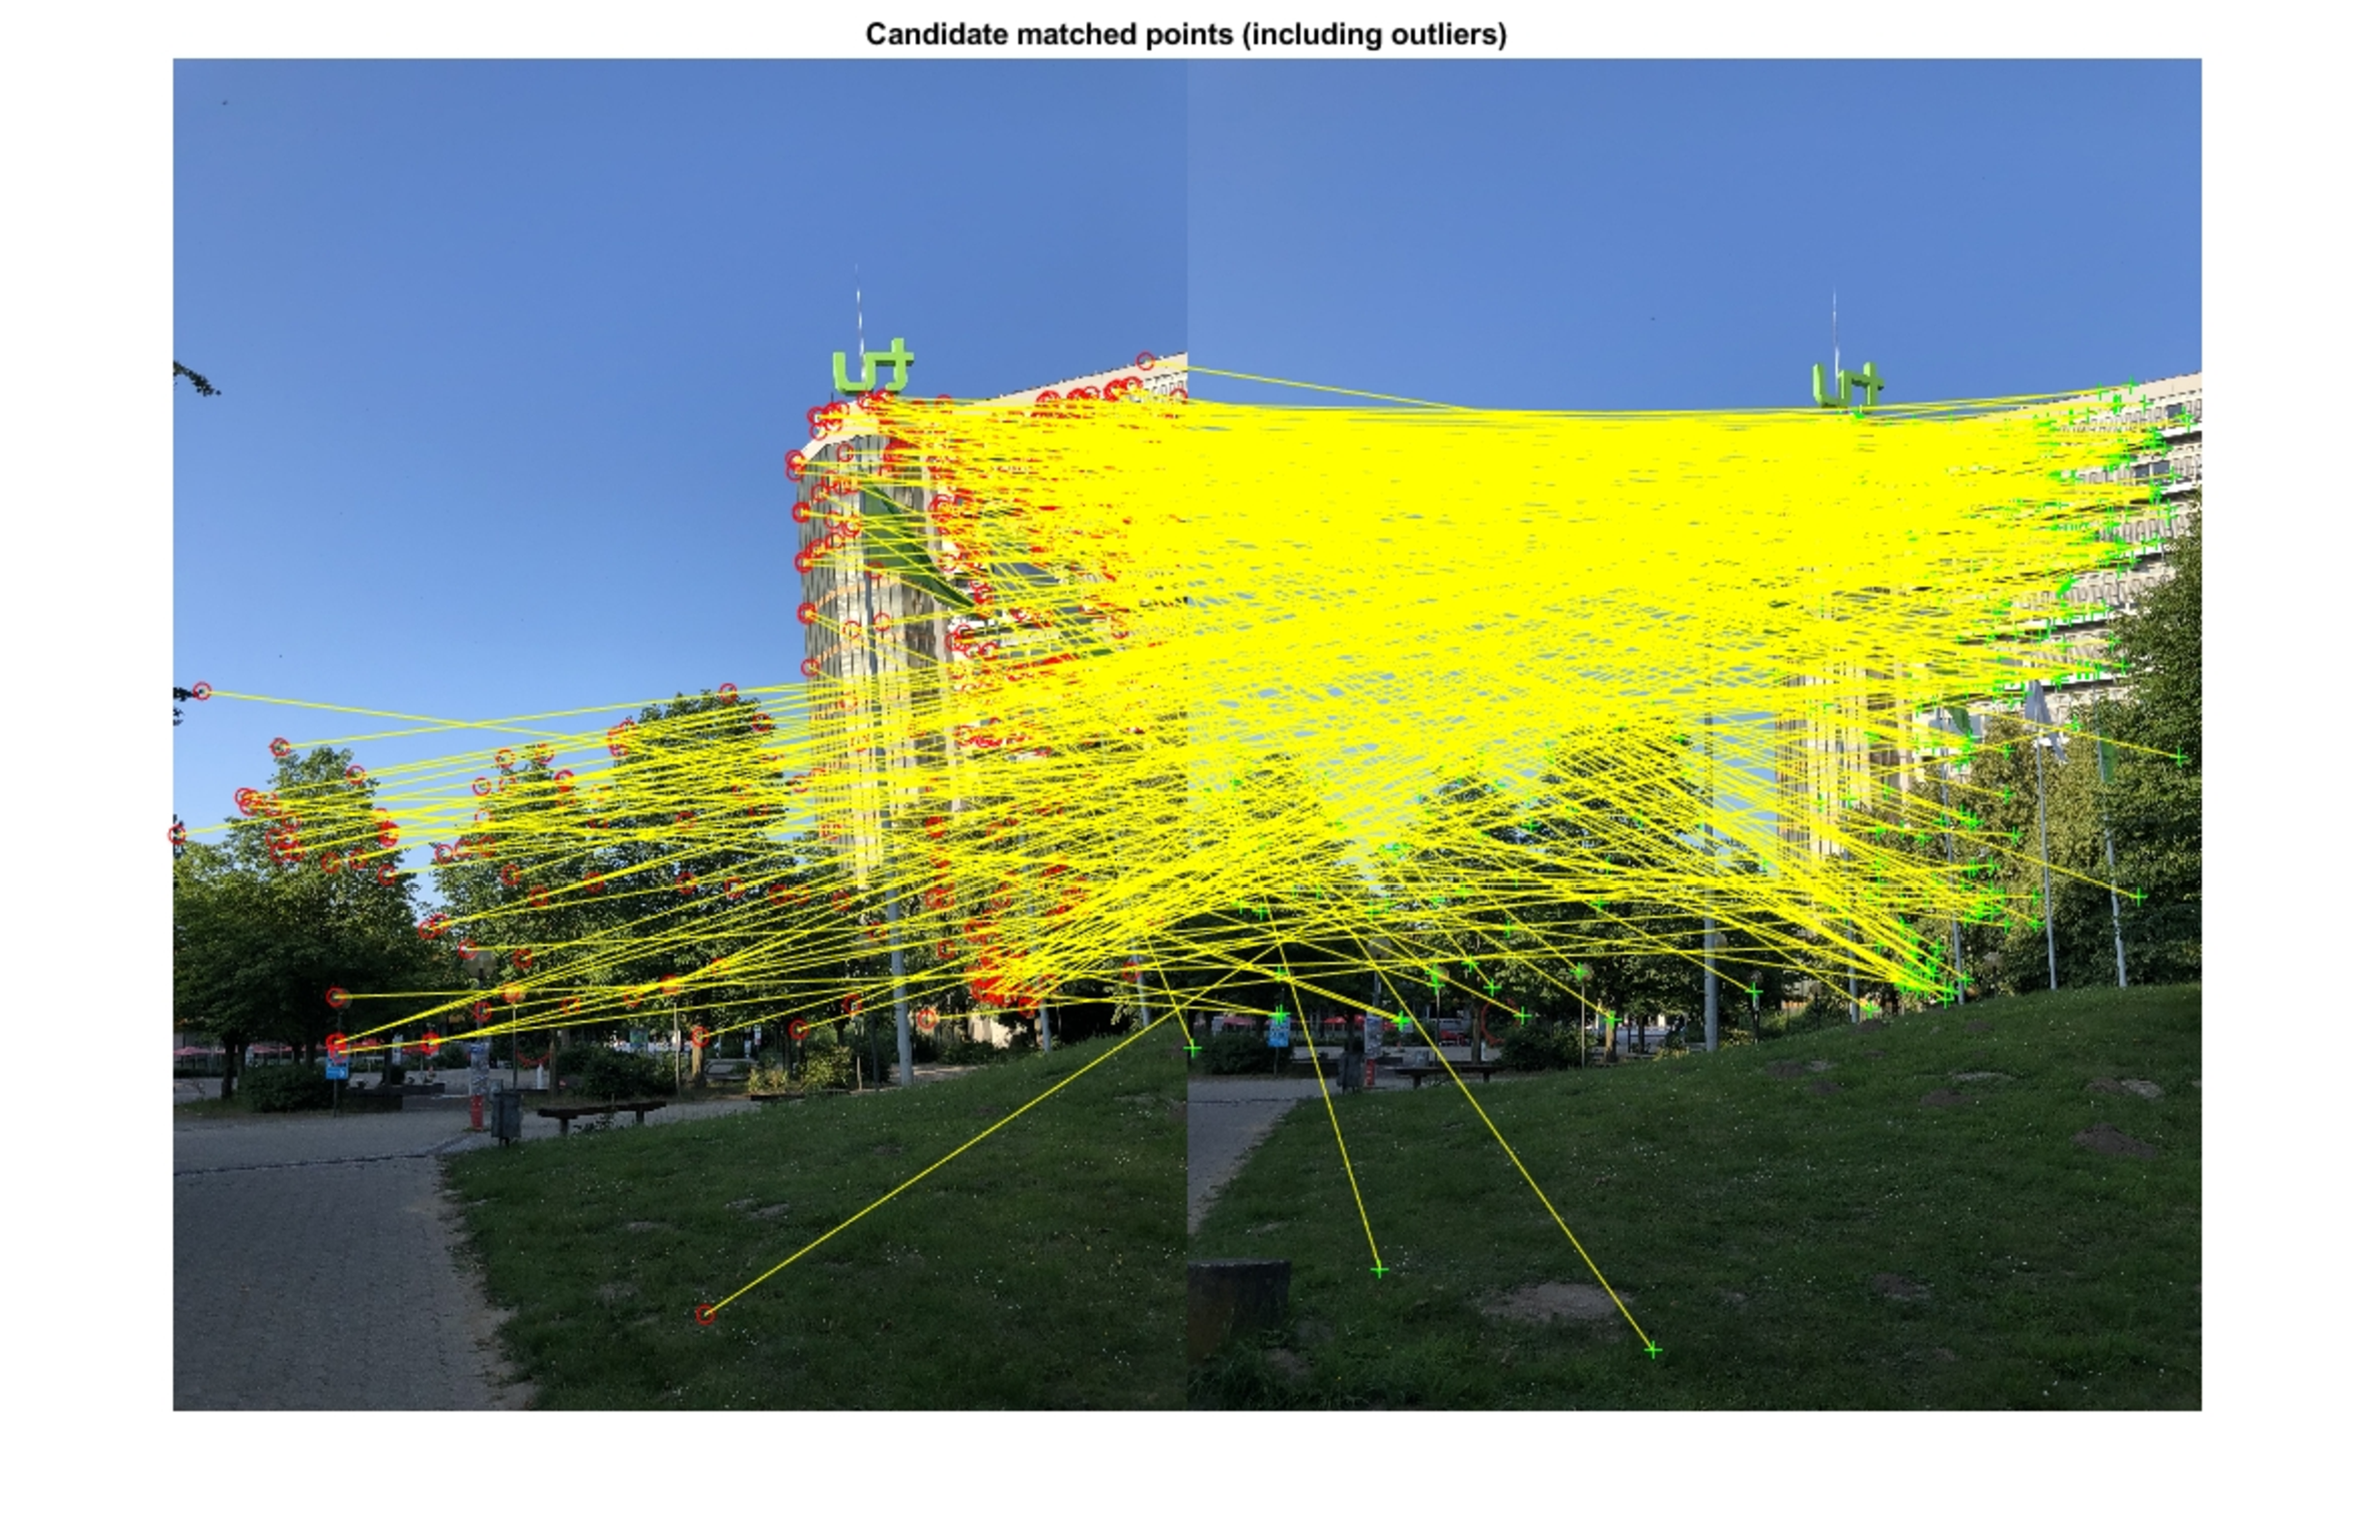
\includegraphics[keepaspectratio,width=0.9\textwidth]{images/3_Ersteverfahren/RANSAC/OhneRANSAC.pdf}
 \caption{Ohne \gls{ransac}}
 \label{fig:OhneRANSAC}
\end{figure} 

\begin{figure}[H]
 \centering 
 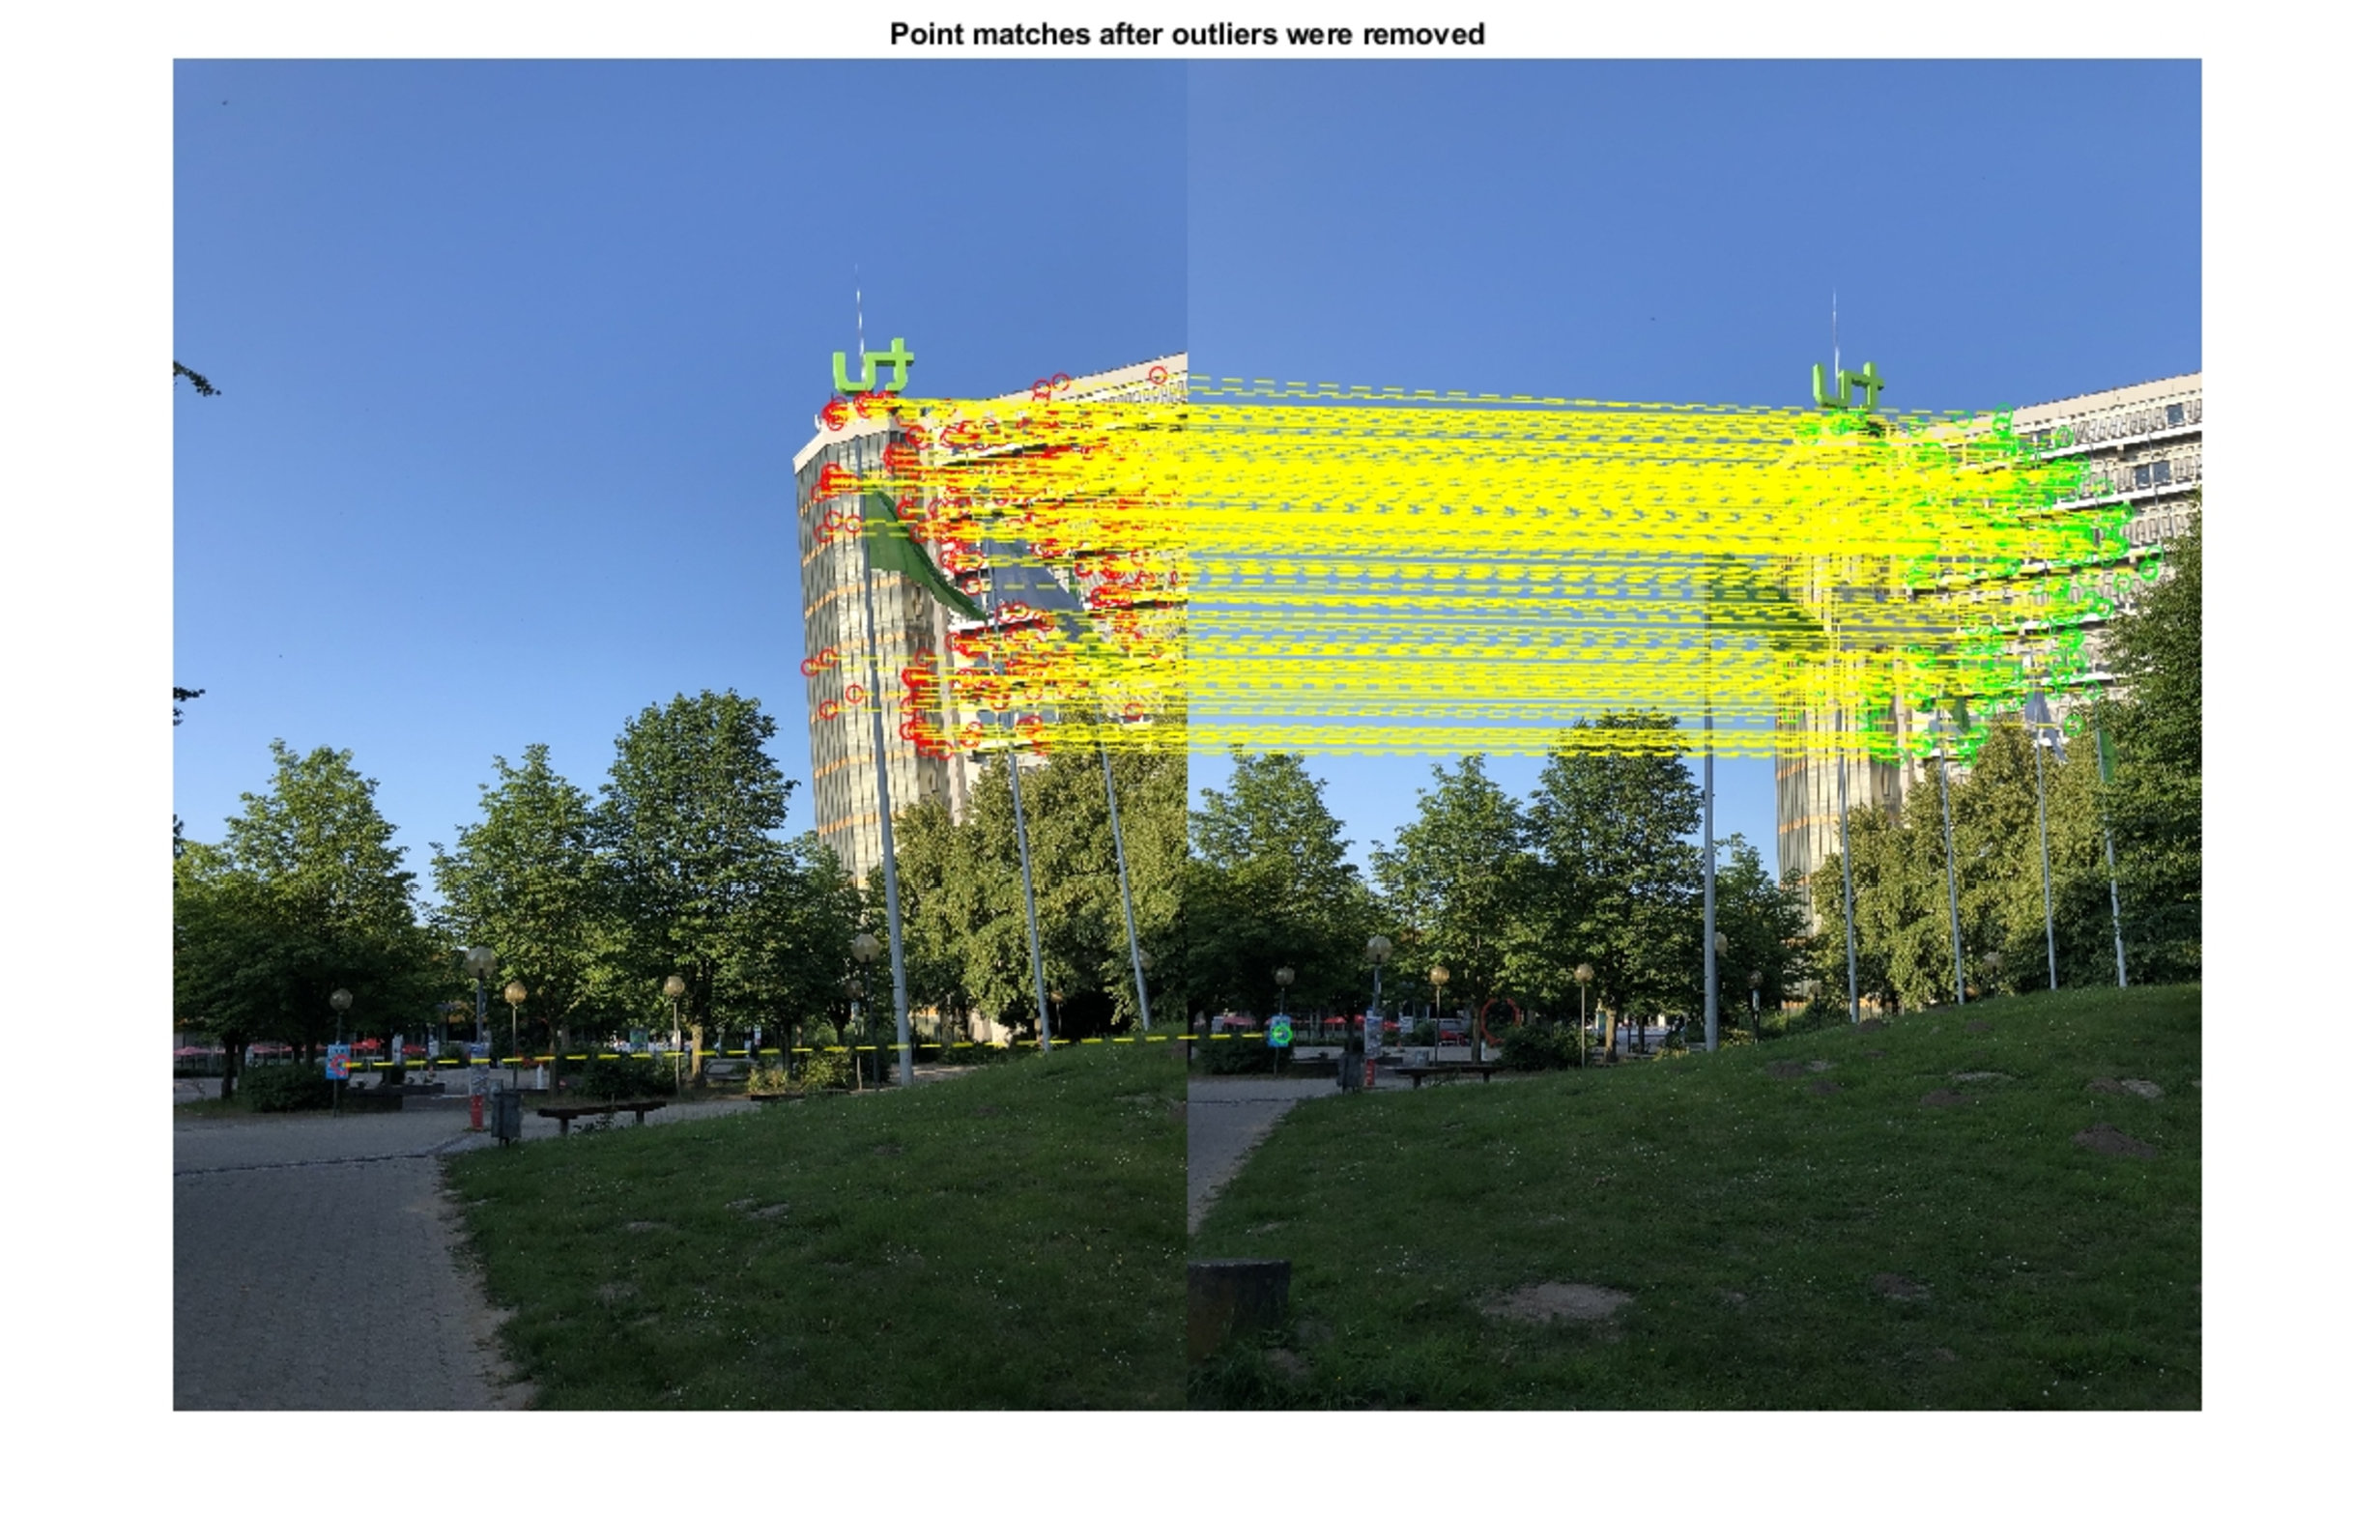
\includegraphics[keepaspectratio,width=0.9\textwidth]{images/3_Ersteverfahren/RANSAC/MitRANSAC.pdf}
 \caption{Mit \gls{ransac}}
 \label{fig:MitRANSAC}
\end{figure} 


\subsection{Bildumwandlung}

Wie in dem vorherigen Abschnitt vorgestellt, kann durch Verwenden des \gls{surf} übereinstimmende Punkte in aufeinanderfolgenden Bildern gefunden werden, anschließend lassen sich durch \gls{ransac} die Ausreißer ausschließen. Das Ziel dieses Abschnitts besteht darin, das Bild in dasselbe Koordinatensystem zu konvertieren. Der erste Schritt ist ein Kameramodell zu erstellen und anschließend die Umwandlungsbeziehung zwischen den entsprechenden Punkten in den zwei Bildern zu erhalten, um schließlich durch den Optimierungsalgorithmus die endgültige Transformationsmatrix zu erhalten. Die verschiedenen Schritte werden im Folgenden detailliert beschrieben.

\textbf{Kamera Modell}

Das Modell der Lochkamera ist in Abbildung \ref{fig:cameramodel} dargestellt. In dem Modell ist $O_C$ das optische Zentrum(Fokus) und f ist die Kamerabrennweite.

\begin{figure}[htb]
 \centering 
 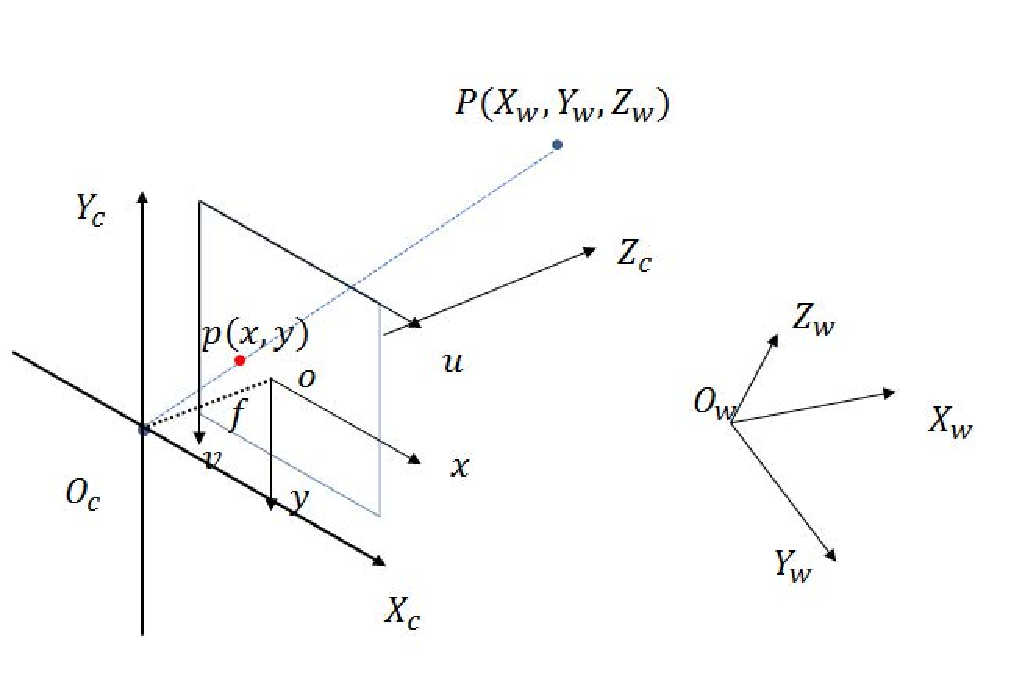
\includegraphics[keepaspectratio,width=0.8\textwidth]{images/3_Ersteverfahren/Kamera/cameramodel.pdf}
 \caption{Modell einer Lochkamera}
 \label{fig:cameramodel}
\end{figure} 

Die vier Koordinatensysteme im Modell sind wie folgt definiert:

\begin{itemize}
	\item 3D Weltkoordinatensystem $P(X_W,Y_W,Z_W)$ \\
	Punktkoordinaten werden durch homogene Koordinaten dargestellt: $\widetilde{X_w}\sim(X_W,Y_W,Z_W,1)^T$
	\item 3D Kamerakoordinatensystem $C(X_C,Y_C,Z_C)$\\
	Punktkoordinaten werden durch homogene Koordinaten dargestellt: $\widetilde{X_c}\sim(X_C,Y_C,Z_C,1)^T$
	\item 2D Bildabbildung Koordinatensystem $p(x,y)$\\
	Punktkoordinaten werden durch homogene Koordinaten dargestellt: $\widetilde{x}\sim(x,y,1)^T$
	\item 2D Bildpixel Koordinatensystem $I(u,v)$\\
	Punktkoordinaten werden durch homogene Koordinaten dargestellt: $\widetilde{u}\sim(u,v,1)^T$
\end{itemize}

% note
Unter diesem Modell wird ein 3D-Punkt im Weltkoordinatensystem durch drei Koordinaten den 2D-Bildpixelkoordinaten zugeordnet.

(\textbf{1}). 3D-Weltkoordinatensystem zum 3D-Kamera-Koordinatensystem.

Die Transformation vom Weltkoordinatensystem zum Kamerakoordinatensystem ist eine Starrekörpertransformation, d.h. das Objekt verformt sich nicht, sondern es rotiert nur und wird parallel verschoben. Diese Transformation wird in Abbildung \ref{fig:WzuC} gezeigt. R ist die Rotationsmatrix und T die Translationsmatrix.

\begin{figure}[htb]
 \centering 
 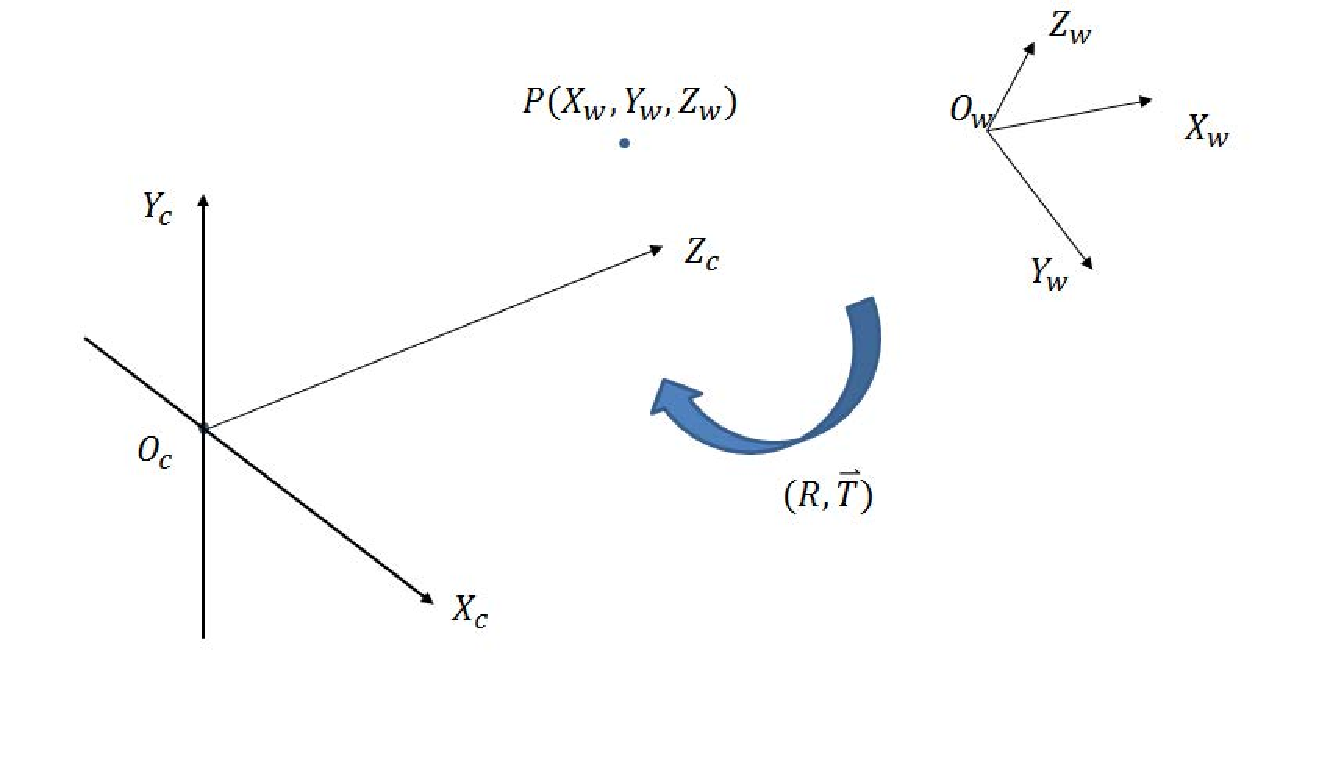
\includegraphics[keepaspectratio,width=0.8\textwidth]{images/3_Ersteverfahren/Kamera/WzuC.pdf}
 \caption{Transformation vom Weltkoordinatensystem zum Kamerakoordinatensystem}
 \label{fig:WzuC}
\end{figure} 

Um die entsprechende Rotationsmatrix zu erhalten, wird die Koordinatenachsen um verschiedene Winkel gedreht. Ein simples Beispiel wird in Abbildung \ref{fig:rotation} gezeigt.

\begin{figure}[H]
 \centering 
 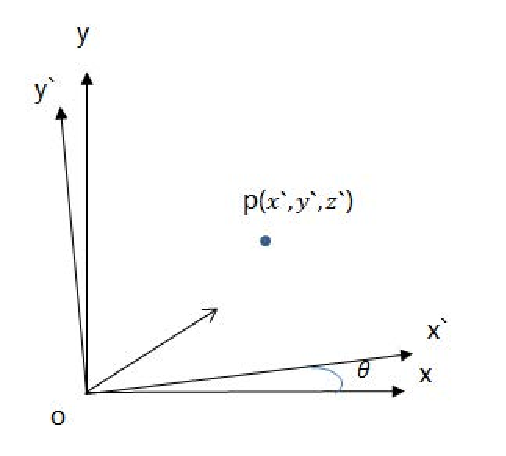
\includegraphics[keepaspectratio,width=0.4\textwidth]{images/3_Ersteverfahren/Kamera/rotationsmatrix.pdf}
 \caption{Rotation um Z-Achse}
 \label{fig:rotation}
\end{figure} 

Aus dem Bild kann leicht entnehmen werden:

\begin{equation}
   \begin{cases} 
	x = x'\cos\theta - y'\sin\theta \\	
	y = x'\sin\theta + y'\cos\theta \\
	z = z'
	\end{cases}
\end{equation}

In Matrixform wie folgt ausgedrückt:

\begin{equation}
   \begin{bmatrix}
	x \\  
	y \\
	z
	\end{bmatrix} = \begin{bmatrix}
	\cos\theta & -\sin\theta & 0	\\
	\sin\theta & \cos\theta  & 0	\\
	0    	   & 0           & 1	
	\end{bmatrix} \cdot \begin{bmatrix}
	x' \\  
	y' \\
	z'
	\end{bmatrix}= R_1 \cdot \begin{bmatrix}
	x' \\  
	y' \\
	z'
	\end{bmatrix}
\end{equation}

In ähnlicher Weise dreht sich die x-Achse, y-Achse um $\varphi$ und $\omega$ Grad wie folgt:

\begin{equation}
   \begin{bmatrix}
	x \\  
	y \\
	z
	\end{bmatrix} = \begin{bmatrix}
		1   & 0          & 0	\\
		0   & \cos\varphi & -\sin\varphi	\\
	    0   & \sin\varphi& \cos\varphi	
	\end{bmatrix} \cdot \begin{bmatrix}
	x' \\  
	y' \\
	z'
	\end{bmatrix}= R_2 \cdot \begin{bmatrix}
	x' \\  
	y' \\
	z'
	\end{bmatrix}
\end{equation}

\begin{equation}
   \begin{bmatrix}
	x \\  
	y \\
	z
	\end{bmatrix} = \begin{bmatrix}
	\cos\omega  & 0           & \sin\omega	\\		
	0    	    & 1           & 0	\\
	-\sin\omega &0            &  \cos\omega
	\end{bmatrix} \cdot \begin{bmatrix}
	x' \\  
	y' \\
	z'
	\end{bmatrix}= R_3 \cdot \begin{bmatrix}
	x' \\  
	y' \\
	z'
	\end{bmatrix}
\end{equation}

Schließlich kann die Rotationsmatrix erhalten werden:
\begin{equation}
   R = R_1 \cdot R_2 \cdot R_3
\end{equation}

Durch das Kombinieren der obigen Ergebnisse, lassen sich die Koordinaten von Punkt P im Kamerakoordinatensystem bestimmen:
\begin{equation}
   \begin{bmatrix}
	X_C \\  
	Y_c \\
	Z_c
	\end{bmatrix} = R \cdot \begin{bmatrix}
	X_w \\  
	Y_w \\
	Z_w 
	\end{bmatrix} +T
\end{equation}

Im homogenen Koordinatensystem dargestellt:
\begin{equation}
   \begin{bmatrix}
	X_C \\  
	Y_C \\
	Z_C \\
	1
	\end{bmatrix} = \begin{bmatrix}
	R & t	\\
	\vec{0}	& 1 \\
	\end{bmatrix} \cdot \begin{bmatrix}
	X_w \\  
	Y_w \\
	Z_w \\
	1
	\end{bmatrix}
\end{equation}

(\textbf{2}). 3D-Kamera-Koordinatensystem zum 2D-Bildabbildung Koordinatensystem.

Die Transformation vom Kamerakoordinatensystem zum Bildkoordinatensystem gehört zur perspektivischen Projektionsbeziehung von 3D zu 2D, wie in Abbildung \ref{fig:Czuimage} gezeigt.

\begin{figure}[H]
 \centering 
 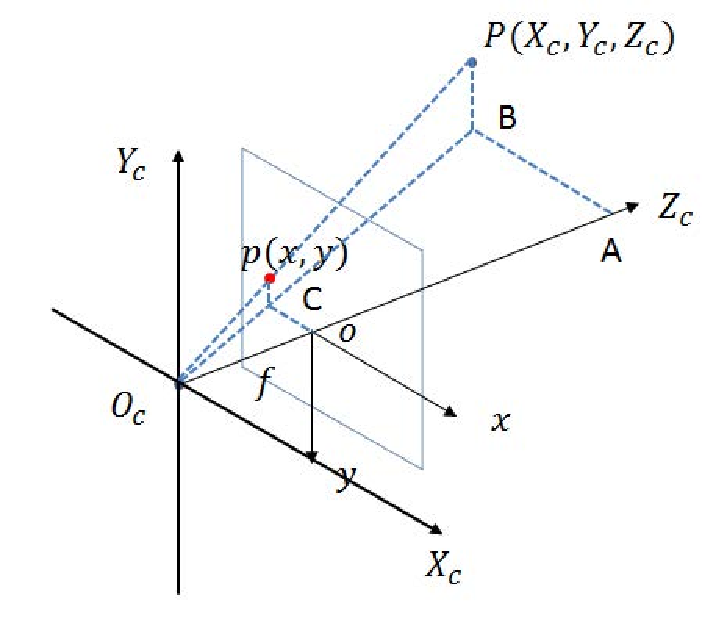
\includegraphics[keepaspectratio,width=0.4\textwidth]{images/3_Ersteverfahren/Kamera/Czuimage.pdf}
 \caption{Transformation vom Kamerakoordinatensystem zum Bildkoordinatensystem}
 \label{fig:Czuimage}
\end{figure} 

Es gibt zwei Paare mit ähnlichen Dreiecken:
\begin{equation}
   \begin{split}
    \triangle ABO_C \sim \triangle oCO_c\\  
	\triangle PBO_C \sim \triangle pCO_c
	\end{split}
\end{equation}

Aus ähnlichen Dreiecksbeziehungen kann diese Gleichung erstellt werden:
\begin{equation}
   \frac{AB}{oC} = \frac{AO_C}{oO_C} = \frac{PB}{pC} = \frac{X_C}{x} = \frac{Z_C}{f} = \frac{Y_C}{y} 
\end{equation}

Durch die Transformationsgleichung folgt: 
\begin{equation}
   x = f \cdot \frac{X_C}{Z_C}, y = f \cdot \frac{Y_C}{Z_C}
\end{equation}

Im homogenen Koordinatensystem dargestellt:
\begin{equation}
   Z_C \cdot \begin{bmatrix}
	x \\  
	y \\
	1
	\end{bmatrix} = \begin{bmatrix}
	f & 0 & 0 & 0	\\
	0 & f & 0 & 0	\\
	0 & 0 & 1 & 0	
	\end{bmatrix} \cdot \begin{bmatrix}
	X_C \\  
	Y_C \\
	Z_C \\
	1
	\end{bmatrix}
\end{equation}

Zu dieser Zeit ist die Einheit des Projektionspunkts p noch nicht Pixel, sondern Millimeter und muss weiter in das Pixelkoordinatensystem umgewandelt werden.

(\textbf{3}). 2D-Bildabbildung Koordinatensystem zum 2D-Bildpixel Koordinatensystem.

Das Pixelkoordinatensystem und das Bildkoordinatensystem befinden sich alle auf der Abbildungsebene, jedoch sind die jeweiligen Ursprünge und Maßeinheiten unterschiedlich. Der Ursprung des Bildkoordinatensystems ist der Schnittpunkt der optischen Achse der Kamera und der Abbildungsebene, üblicherweise der Mittelpunkt der Abbildungsebene oder der Hauptpunkt. Die Einheit des Bildkoordinatensystems ist Millimeter welche eine physikalische Einheit ist. Die Einheit des Pixelkoordinatensystems ist Pixel. Wie gewohnt wird beschrieben in welcher Zeile und Spalte ein Pixel ist. So ist der Übergang zwischen den beiden Koordinatensystem wie in Abbildung \ref{fig:Konvertierung von Pixelkoordinatensystem zu Bildkoordinatensystem} dargestellt. 

\begin{figure}[H]
 \centering 
 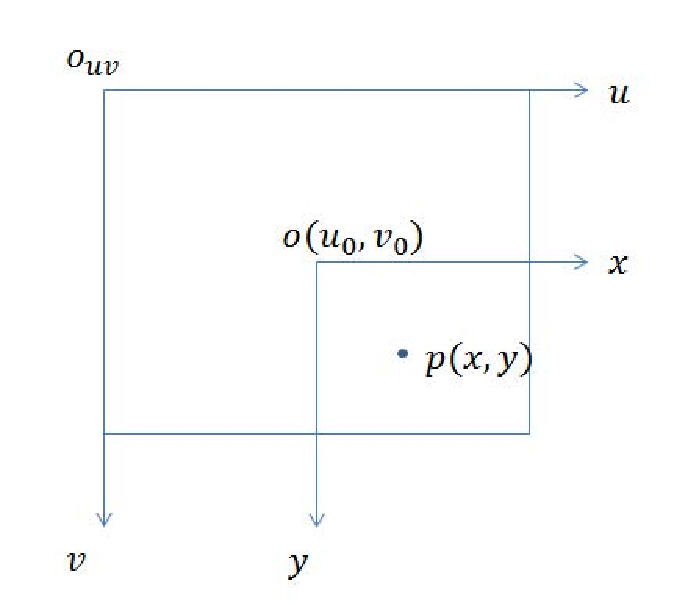
\includegraphics[keepaspectratio,width=0.5\textwidth]{images/3_Ersteverfahren/Kamera/imagezupixel.pdf}
 \caption{Konvertierung vom Bildkoordinatensystem zum Pixelkoordinatensystem}
 \label{fig:Konvertierung von Pixelkoordinatensystem zu Bildkoordinatensystem}
\end{figure} 

$d_x$ und $d_y$ ist die Größe jedes Pixel in den X- und Y-Achsenrichtungen. Jedes Pixel des Bildes hat die folgende Beziehung zwischen den zwei Koordinatensystemen.

\begin{equation}
   \begin{cases} 
	u = \frac{x}{d_x} + u_0	 \\  
	v = \frac{y}{d_y} + v_0	
	\end{cases}
\end{equation}

Im homogenen Koordinatensystem dargestellt:

\begin{equation}
   \begin{bmatrix}
	u \\  
	v \\
	1
	\end{bmatrix} = \begin{bmatrix}
	\frac{1}{d_x} 			& 0 			& u_0	\\
	0	 					& \frac{1}{d_y} & v_0	\\
	0     					& 0 			& 1	
	\end{bmatrix} \cdot \begin{bmatrix}
	x \\  
	y \\
	1
	\end{bmatrix}
\end{equation}

Es ist erwähnenswert, dass das Bildkoordinatensystem eine zweidimensionale Ebene(Bildebene), praktisch die Oberfläche des Kamera-CCD-Sensors ist. Jeder CCD-Sensor hat eine bestimmte Größe und Auflösung. Diese beiden Faktoren bestimmen die Konvertierungsbeziehung. Gegeben sei ein simples Beispiel: Eine Größe des CCD-Sensors ist $\SI{8}{\mm} \times \SI{6}{\mm}$, die Auflösung dafür ist $640~pixels \times 480~pixels$. Die Beziehung zwischen mm und Pixel ist $80~pixel/mm$. Ist die physikalische Größe jedes Pixels des CCD-Sensors $d_x \times d_y$, entspricht diese $d_x = d_y = \SI{1/80}{\mm}$.
 
Durch die Umwandlung der obigen vier Koordinatensysteme kann ein Punkt vom Weltkoordinatensystem zum Pixelkoordinatensystem extrahiert werden.
\begin{equation}
\begin{split}
   Z_C \cdot \begin{bmatrix}
	u \\  
	v \\
	1
	\end{bmatrix} & = \begin{bmatrix}
	\frac{1}{d_x} 			& 0 			& u_0	\\
	0	 					& \frac{1}{d_y} & v_0	\\
	0     					& 0 			& 1	
	\end{bmatrix} \cdot \begin{bmatrix}
	f & 0 & 0 & 0	\\
	0 & f & 0 & 0	\\
	0 & 0 & 1 & 0	
	\end{bmatrix} \cdot \begin{bmatrix}
	R & t	\\
	\vec{0}	& 1 \\
	\end{bmatrix} \cdot \begin{bmatrix}
	X_w \\  
	Y_w \\
	Z_w \\
	1
	\end{bmatrix} \\
	& = \begin{bmatrix}
	f_x & 0 & u_0 & 0	\\
	0 & f_y & v_0 & 0	\\
	0 & 0 & 1 & 0	
	\end{bmatrix} \cdot \begin{bmatrix}
	R & t	\\
	\vec{0}	& 1 \\
	\end{bmatrix} \cdot \begin{bmatrix}
	X_w \\  
	Y_w \\
	Z_w \\
	1
	\end{bmatrix}
\end{split}	
\end{equation}

Die erste Matrix der rechten Gleichung ist die allgemein bekannte interne Referenz der Kamera. Dagegen ist die zweite Matrix die externe Referenz der Kamera. Beide Parameter der Kamera können durch Zhang Zhengyou \cite{zhangzhengyou} Kalibrierung erhalten werden. Einige typische Kamera Parameter vom Werk aus sind der Tabellen \ref{tbl:Parameter der Kameras im Vergleich} zu entnehmen.

\begin{table}[htb]
	\captionabove{Parameter der Kameras im Vergleich}
	\label{tbl:Parameter der Kameras im Vergleich}
	\footnotesize
	\centering
	\rowcolors{2}{white}{gray!25}	%TUgreen!25
	\begin{tabular}{|p{3cm}|p{2.5cm}|p{2.5cm}|p{2.5cm}|}	%p{}m{}b{}clr
	\toprule
	\textbf{Parameter} & \textbf{Google Pixel} & \textbf{Google Pixel2} & \textbf{Iphone X}\\
	\midrule
	Sensor Größe $''$ & 1/2.3 & 1/2.6 & 1/3 \\
	Bild Auflösung $pixels$ & $4048 \times 3036$ & $4032 \times 3024$ & $4032 \times 3024$ \\
	Pixel Größe $\mu m$ & 1.544 & 1.4 & 1.22 \\	
	Brennweite $mm$ & 4.67 & 4.47 & 3.99 \\
	Formatfaktor $35 mm$  	&5.55	&6.04	&7.02	\\
	
	\bottomrule
	\end{tabular}
\end{table} 


Wenn die internen und externen Parameter der Kamera bekannt sind, ist es möglich daraus die Projektionsmatrix zu erstellen um daraus die Bildkoordinaten jeden beliebigen räumlichen Punkts zu erhalten. Wenn die Position $m(u,v)$ einer Bildkoordinate und die Parameter innerhalb und außerhalb der Kamera bekannt sind, kann der entsprechende Punkt in Weltkoordinate nur ungefähr bestimmt werden. Der Grund dafür ist, dass die $Z_c$ Information während des Projektionsprozesses eliminiert wird. 

\textbf{Umwandlungsmodelle}

Als nächstes wird die Umwandlungsbeziehung zwischen den entsprechenden Punkten in den beiden Bilder vorgenommen. Zuerst wird in dieser Arbeit eine vereinfachte Situation betrachtet, d.h. nur mit Rotationseinfluss. Abbildung \ref{fig:rotationsmodel} zeigt das 3D-Rotationsbewegungsmodell der Kamera. Die Position des optischen Zentrums ändert sich, während der Kamerabewegung im Drehbewegungsmodell der Kamera, nicht. Unter diesem Modell ist die Abbildungsbeziehung zwischen dem Punkt X im Weltkoordinatensystem und der Bildkoordinate x im homogenen Koordinatensystem dargestellt: 
\begin{equation}
   x = KRX, X = \lambda  K^{-1} x
\end{equation}

Wobei K der interne Parameter der Kamera ist, wie zuvor definiert. $\lambda$ ist der unbekannte Skalierungsfaktor, d.h. dass unter dem Kameramodell die Quelle jeder Bildpunktkoordinate einem Strahl zugeordnet ist.

\begin{figure}[H]
 \centering 
 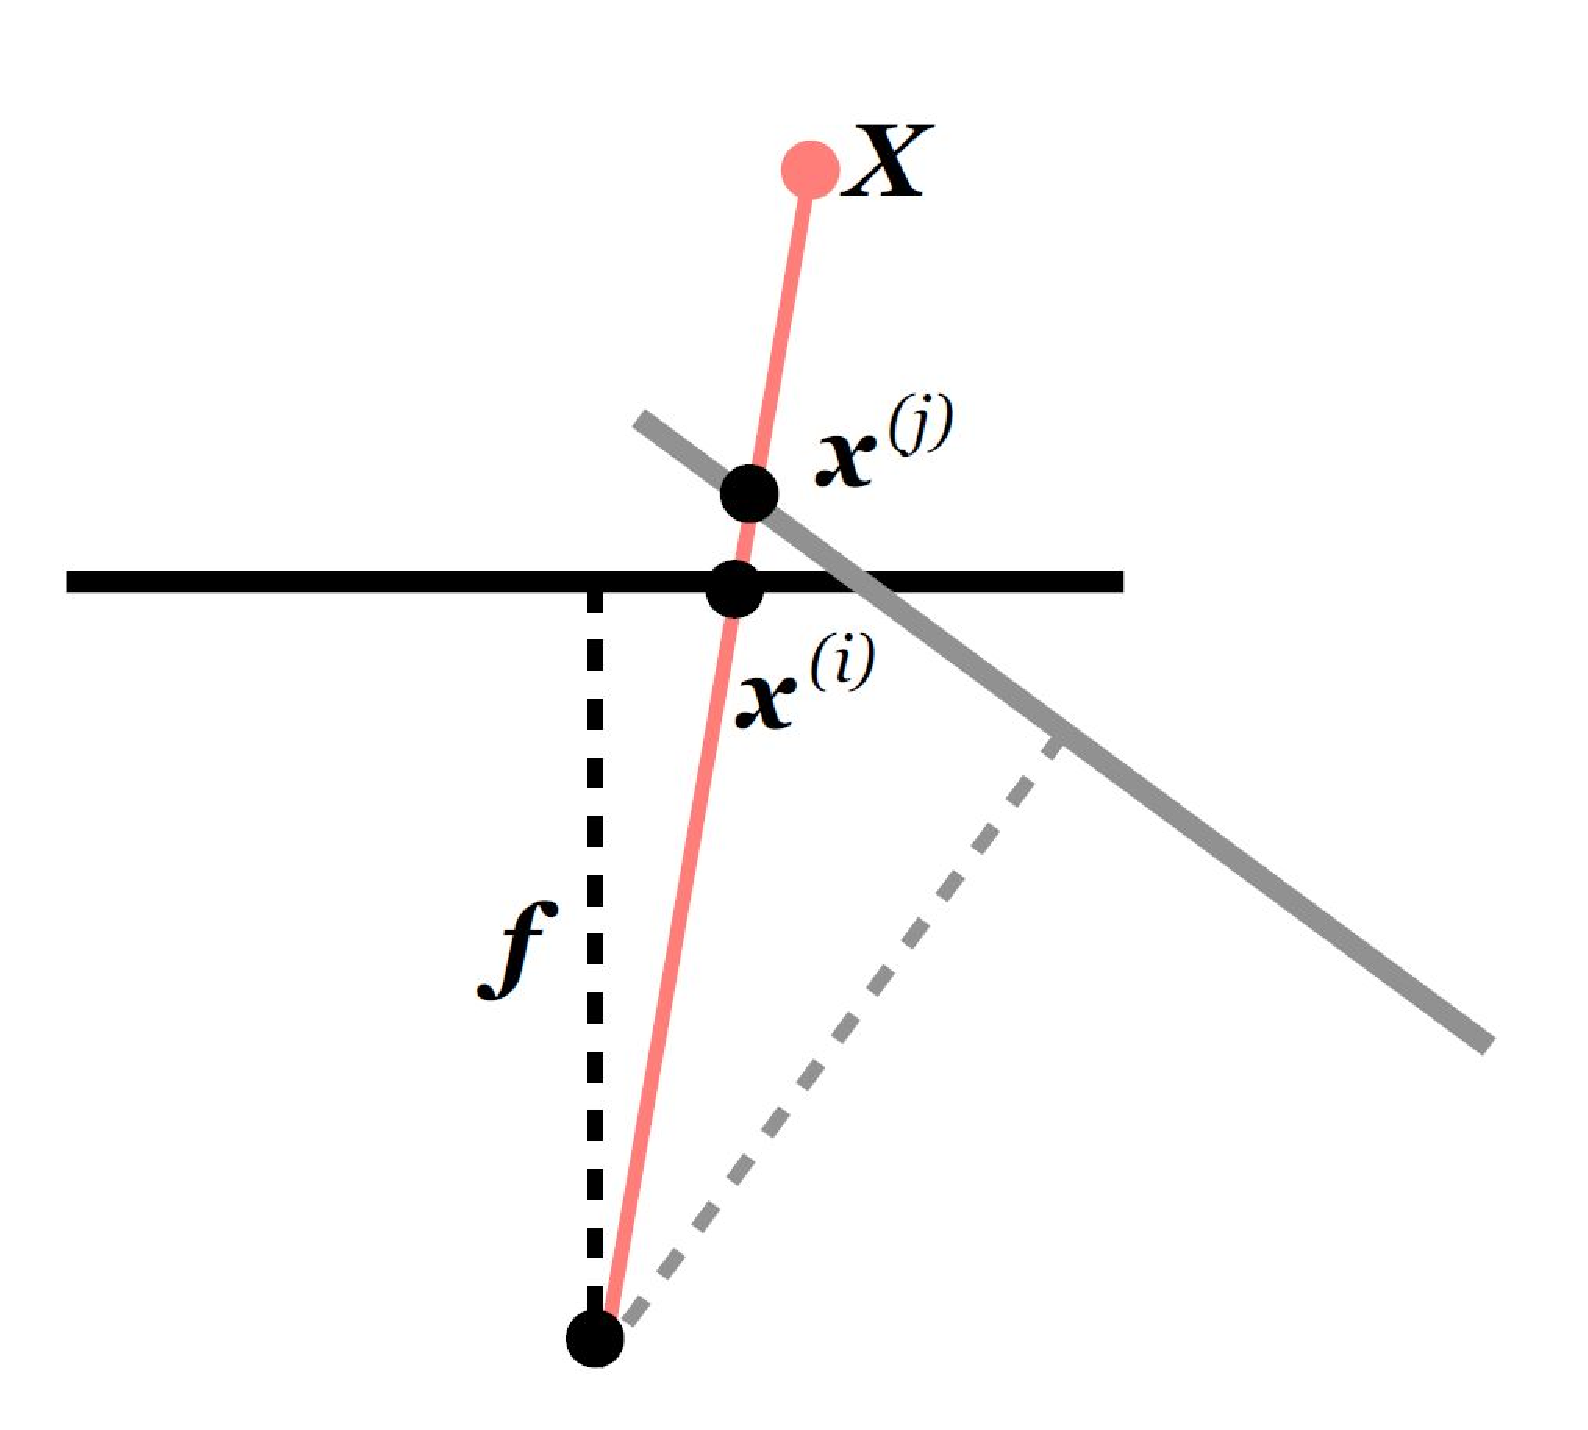
\includegraphics[keepaspectratio,width=0.5\textwidth]{images/3_Ersteverfahren/Kamera/rotationsmodel.pdf}
 \caption{Rotationsbewegungsmodell}
 \label{fig:rotationsmodel}
\end{figure} 

Nun wird die Beziehung zwischen Bildpunkten in einem Framepaar zwei verschiedener Kameraausrichtungen hergeleitet(siehe Abbildung \ref{fig:rotationsmodel}). Für einen Weltkoordinatepunkt X sind die projizierten Punkte $x_i$ und $x_j$ in der Bildebene von zwei Bildern i und j gegeben durch
\begin{equation}
   x_i = KR_iX, x_j = KR_jX
\end{equation}

Nach weiterem anordnen und ersetzen von X, wird eine Beziehung aller Punkte im Bildrahmen i auf alle Punkte im Rahmen j erhalten:
\begin{equation}
   x_j = KR_jR_i^TK^{-1}x_i
\end{equation}

Bisher wurde nur die Beziehung zwischen zwei Bildern der selben Aufnahme betrachtet. Diese Einschränkung wird gelockert, indem Frames von einer Kamera, die sich gemäß $R$ dreht, zu einer anderen Kamera, die sich gemäß $R'$ dreht, abgebildet werden. Es gibt eine Hypothese, dass beide Kamerazentren sich im Ursprung befinden. Mit der Warping-Matrix können die abgebildeten Punkte der Kameras wie folgt definiert werden:
\begin{equation}
   W = KR'R^TK^{-1}
\end{equation}

Hier wird das erste Bild als Referenzbild mit einem Rotationswinkel von 0 Grad gewählt, wodurch die Gleichung vereinfacht werden kann:
\begin{equation}
   W = KRK^{-1}
\end{equation}

Kombiniert mit Formel 3.23 kann es ausgedrückt werden als:
\begin{equation}
   x_j = Wx_i
\end{equation}

Diese Gleichung zeigt, dass jeder Punkt in dem Bild i nach der Transformationsmatrix W in einen entsprechenden Punkt in dem Bild j umgewandelt werden kann. Weiter in einem allgemeineren Fall, d.h. von nun an nicht nur mit Rotationseinfluss, sondern auch Translationseinfluss. Der Ableitungsverlauf ist im Allgemeinen gleich. Der Hauptunterschied ist die Anzahl der Parameter, die ursprünglich nur 3 Rotationsparameter aber jetzt 6 Parameter einschließlich 3 Rotationsparameter und 3 Translationsparameter beinhalten. Die neue Warping-Matrix sieht folgendermaßen aus:

\begin{equation}
   W = \begin{bmatrix}
	f			& 0 		& \frac{w}{2}	  & 0 \\
	0	 		& f			& \frac{h}{2} 	  & 0 \\
	0     		& 0 		& 1 			  & 0 \\	
	0     		& 0 		& 0 			  & 1
	\end{bmatrix} \cdot \begin{bmatrix}
	R_{11}			& R_{21}  		& R_{31}	  & 0 \\
	R_{12}	 		& R_{22}		& R_{32}	  & 0 \\
	R_{13}     		& R_{23} 		& R_{33} 	  & 0 \\	
	t1     			& t2 			& t3 		  & 1
	\end{bmatrix} \cdot \begin{bmatrix}
	\frac{1}{f}	   & 0 				& -\frac{w}{2f}	  & 0 \\
	0	 		   & \frac{1}{f}	& -\frac{h}{2f}   & 0 \\
	0     		   & 0 		        & 1 			  & 0 \\	
	0     		   & 0 		        & 0 			  & 1
	\end{bmatrix}
\end{equation}

\textbf{Transformationsoptimierung}

In den letzten beiden Abschnitten wurde die Transformationsmatrix zwischen den beiden Bildern aus dem Kameramodell abgeleitet. Hier in diesem Abschnitt werden die Parameter der Transformationsmatrix berechnet, also wird nun die Transformationsmatrix bestimmt. Hier sind die entsprechenden Punkte von zwei benachbarten Bildern $x_i, x_j$ bekannt und die Umwandlungsbeziehung dazwischen wird als die Formel 3.26 dargestellt. Angesichts dieser Bedingung 
kann die Berechnung der Transformationsmatrix als ein Optimierungsproblem betrachtet werden, wobei der Fehler J bei der Summenwertbildung im Quadrat aller Punktkorrespondenzen minimiert werden soll:

\begin{equation}
   J = \sum_{(i,j)}\lVert x_j - Wx_i \rVert ^2
\end{equation}

Zu Beachten ist, dass dies ein nichtlineares Optimierungsproblem ist. Einige nichtlineare Optimierer können ebenfalls verwendet werden um diese Zielfunktion zu minimieren. In der Kapital Evaluierung wurde bewissen, dass der Koordinatenabstieg durch direkte objektive Funktionsbewertung schnell konvergiert. Jedes Mal, wenn ein Schritt gemacht wird bei dem die Zielfunktion J nicht abnimmt, wird die Schrittrichtung umgekehrt und verringert die Schrittweite des entsprechenden Parameters. Der Algorithmus endet, sobald die Schrittgröße für alle Parameter unter einen gewünschten Schwellenwert fällt (d.h. Wenn die Zielgenauigkeit erreicht ist). 

Der detaillierte Algorithmus ist wie folgt dargestellt. Einige Definitionen werden hier eingeführt. $P_0$ ist der Vektor, der die Anfangswerte der Parameter speichert. Anschießend speichert er die Schrittgröße jedes Parameters in den Vektor $d_p$. $temp_dp$ ist der Vektor, in dem die gewünschten Schwellenwerte der Parameter gespeichert werden. D ist die Anzahl Unbekannter Parameter und W die Transformationsmatrix.

\textbf{1}. Zuerst durch Anfangswert $P_0$ Berechnung des anfänglichen Fehlers $J_0$.

\textbf{2}. Veränderung eines Parameters in eine entsprechende Schrittrichtung mit entsprechender Schrittgröße.

\textbf{3}. Berechnung der neuen Fehler $J_{new}$.

\textbf{4}. Vergleichen der beiden Fehler, ob der neue Fehler $J_{new}$ kleiner ist. Wenn Ja wird dieser neue Wert beibehalten. Wenn Nein wird die Schrittrichtung umgekehrt und die Schrittgröße auf ein Drittel des vorherigen Werts reduziert. Dann ändern das Objekt auf den nächsten Parameter und kehren zum zweiten Schritt zurück.

\textbf{5}. Wenn alle Schrittgrößen in $d_p$ den zuvor festgelegten Schwellenwert erreichen, wird der Algorithmus, mit Ausgabe des minimalen Fehlers J und der entsprechenden Transformationsmatrix, terminiert.

Das Flussdiagramm des Algorithmus ist wie in Abbildung \ref{fig:FlussdiagrammforOptimierung} dargestellt.

Durch die Transformationsmatrix können die Koordinaten des zweiten Bildes in die Koordinaten des ersten Bildes übertragen werden. Abbildung \ref{fig:Transformation in eine Koordinate} zeigt diesen Verlauf. Schließlich kann durch Subtraktion das Differenzbild erzeugt werden.

\begin{figure}[H]
 \centering 
 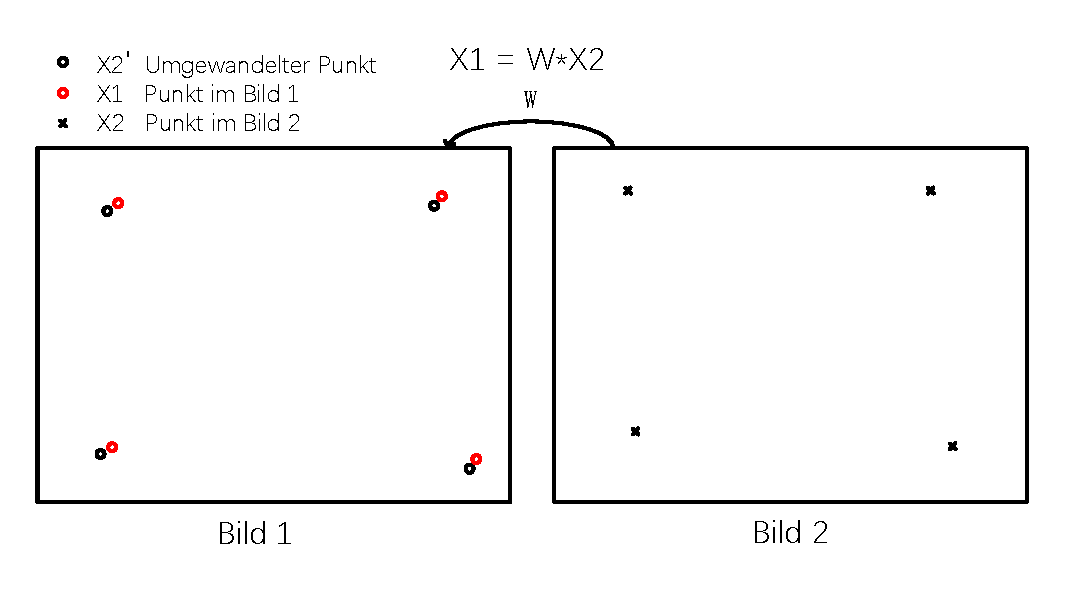
\includegraphics[keepaspectratio,width=0.8\textwidth]{images/3_Ersteverfahren/Kamera/Transformmatrix.pdf}
 \caption{Transformation in das selbe Koordinatensystem}
 \label{fig:Transformation in eine Koordinate}
\end{figure} 

\begin{figure}[H]
 \centering 
 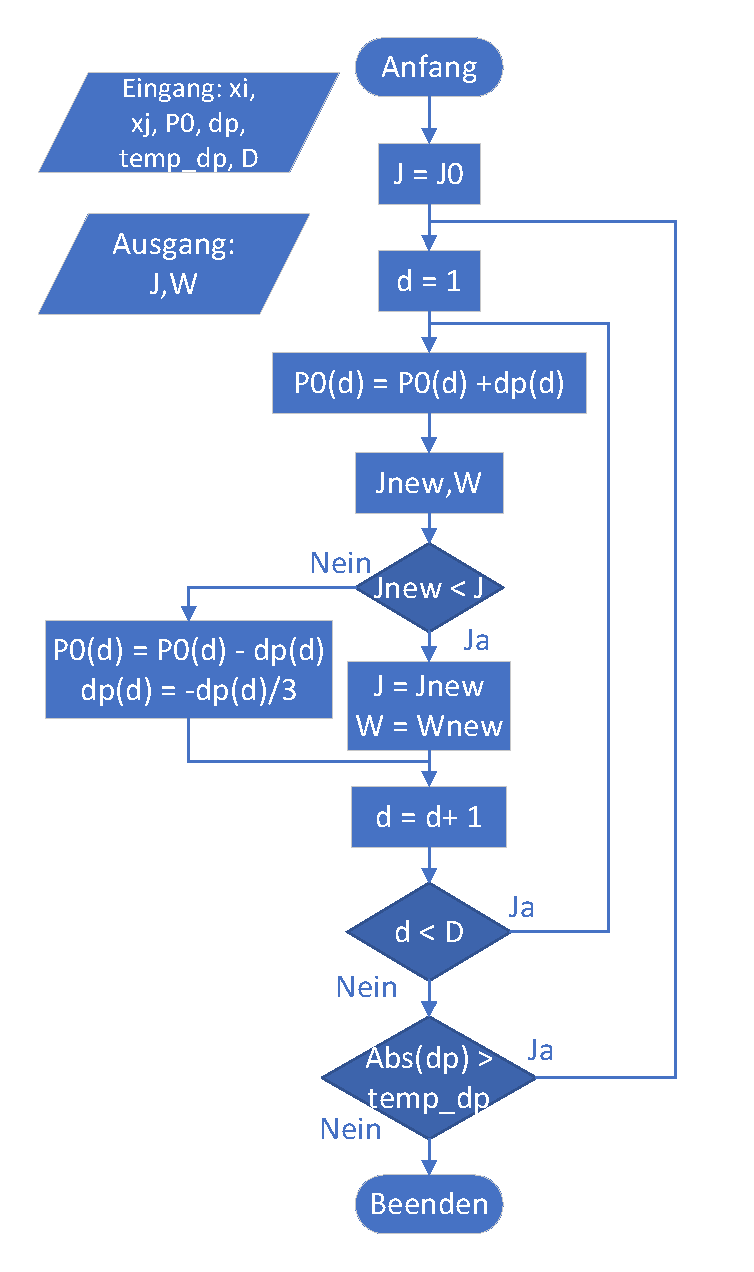
\includegraphics[keepaspectratio,width=0.8\textwidth]{images/3_Ersteverfahren/Kamera/flussdiagramm_for_parameter.pdf}
 \caption{Flussdiagramm für Optimierung}
 \label{fig:FlussdiagrammforOptimierung}
\end{figure} 



\section{Differenzbild-Optimierung}
Die Bildregistration liefert eine Reihe Bilder von der Kamera, deren Koordinaten in dasselbe Koordinatensystem umgewandelt wurden. Es werden je zwei Bilder ausgewählt und subtrahiert, um eine Reihe Differenzbilder zu erhalten. Das Ziel in diesem Abschnitt ist, von diesen Differenzbildern ein zu detektierendes Bild herzustellen, das die QR Muster Detektion vereinfacht. Es sollte hier beachtet werden, dass aufgrund der Zeitsynchronisation die QR Muster in den Differenzbildern einige unerwartete Effekte aufweisen könnten. Eine mögliche Formel der Differenzbilder wie folgt mit der Anhahme dass es in vertikaler Richtung ist.

\begin{itemize}
	\item total Schwarz-Weiß-Schwarz-Weiß-Schwarz Ordnung.
	\item halb Schwarz-Weiß-Schwarz-Weiß-Schwarz Ordnung, halb nicht gezeigt.
	\item total Weiß-Schwarz-Weiß-Schwarz-Weiß Ordnung.
	\item halb Weiß-Schwarz-Weiß-Schwarz-Weiß Ordnung, halb nicht gezeigt.
	\item halb Schwarz-Weiß-Schwarz-Weiß-Schwarz Ordnung, halb Weiß-Schwarz-Weiß-Schwarz-Weiß Ordnung.
	\item total nicht gezeigt.
\end{itemize}

Tabelle \ref{tbl:differenzbildformel} zeigt solche Situationen und listet auf, ob sie zur folgenden Detektion angepasst sind. Die direkte Verwendung dieser Differenzbilder ist für die nächste Detektion ein kniffliges Problem. Um dieses Problem zu lösen, wurde ein Algorithmus zur Optimierung der Differenzbilder entwickelt.

\begin{table}[htb]
	\captionabove{mögliche Differenzbilder}
	\label{tbl:differenzbildformel}
	\footnotesize
	\centering
	\rowcolors{2}{white}{gray!25}	%TUgreen!25
	\begin{tabular}{|p{2cm}<{\centering}|c|p{2cm}<{\centering}|c|}	%p{}m{}b{}clr p{3cm} p{8cm}
	\toprule
	\textbf{Ob angepasst zu folgender Detektion?} & \multirow{4}{*}{\textbf{Differenzbild}} & \textbf{Ob angepasst zu folgender Detektion?} & \multirow{4}{*}{\textbf{Differenzbild}} \\
	\midrule
	 Ja & 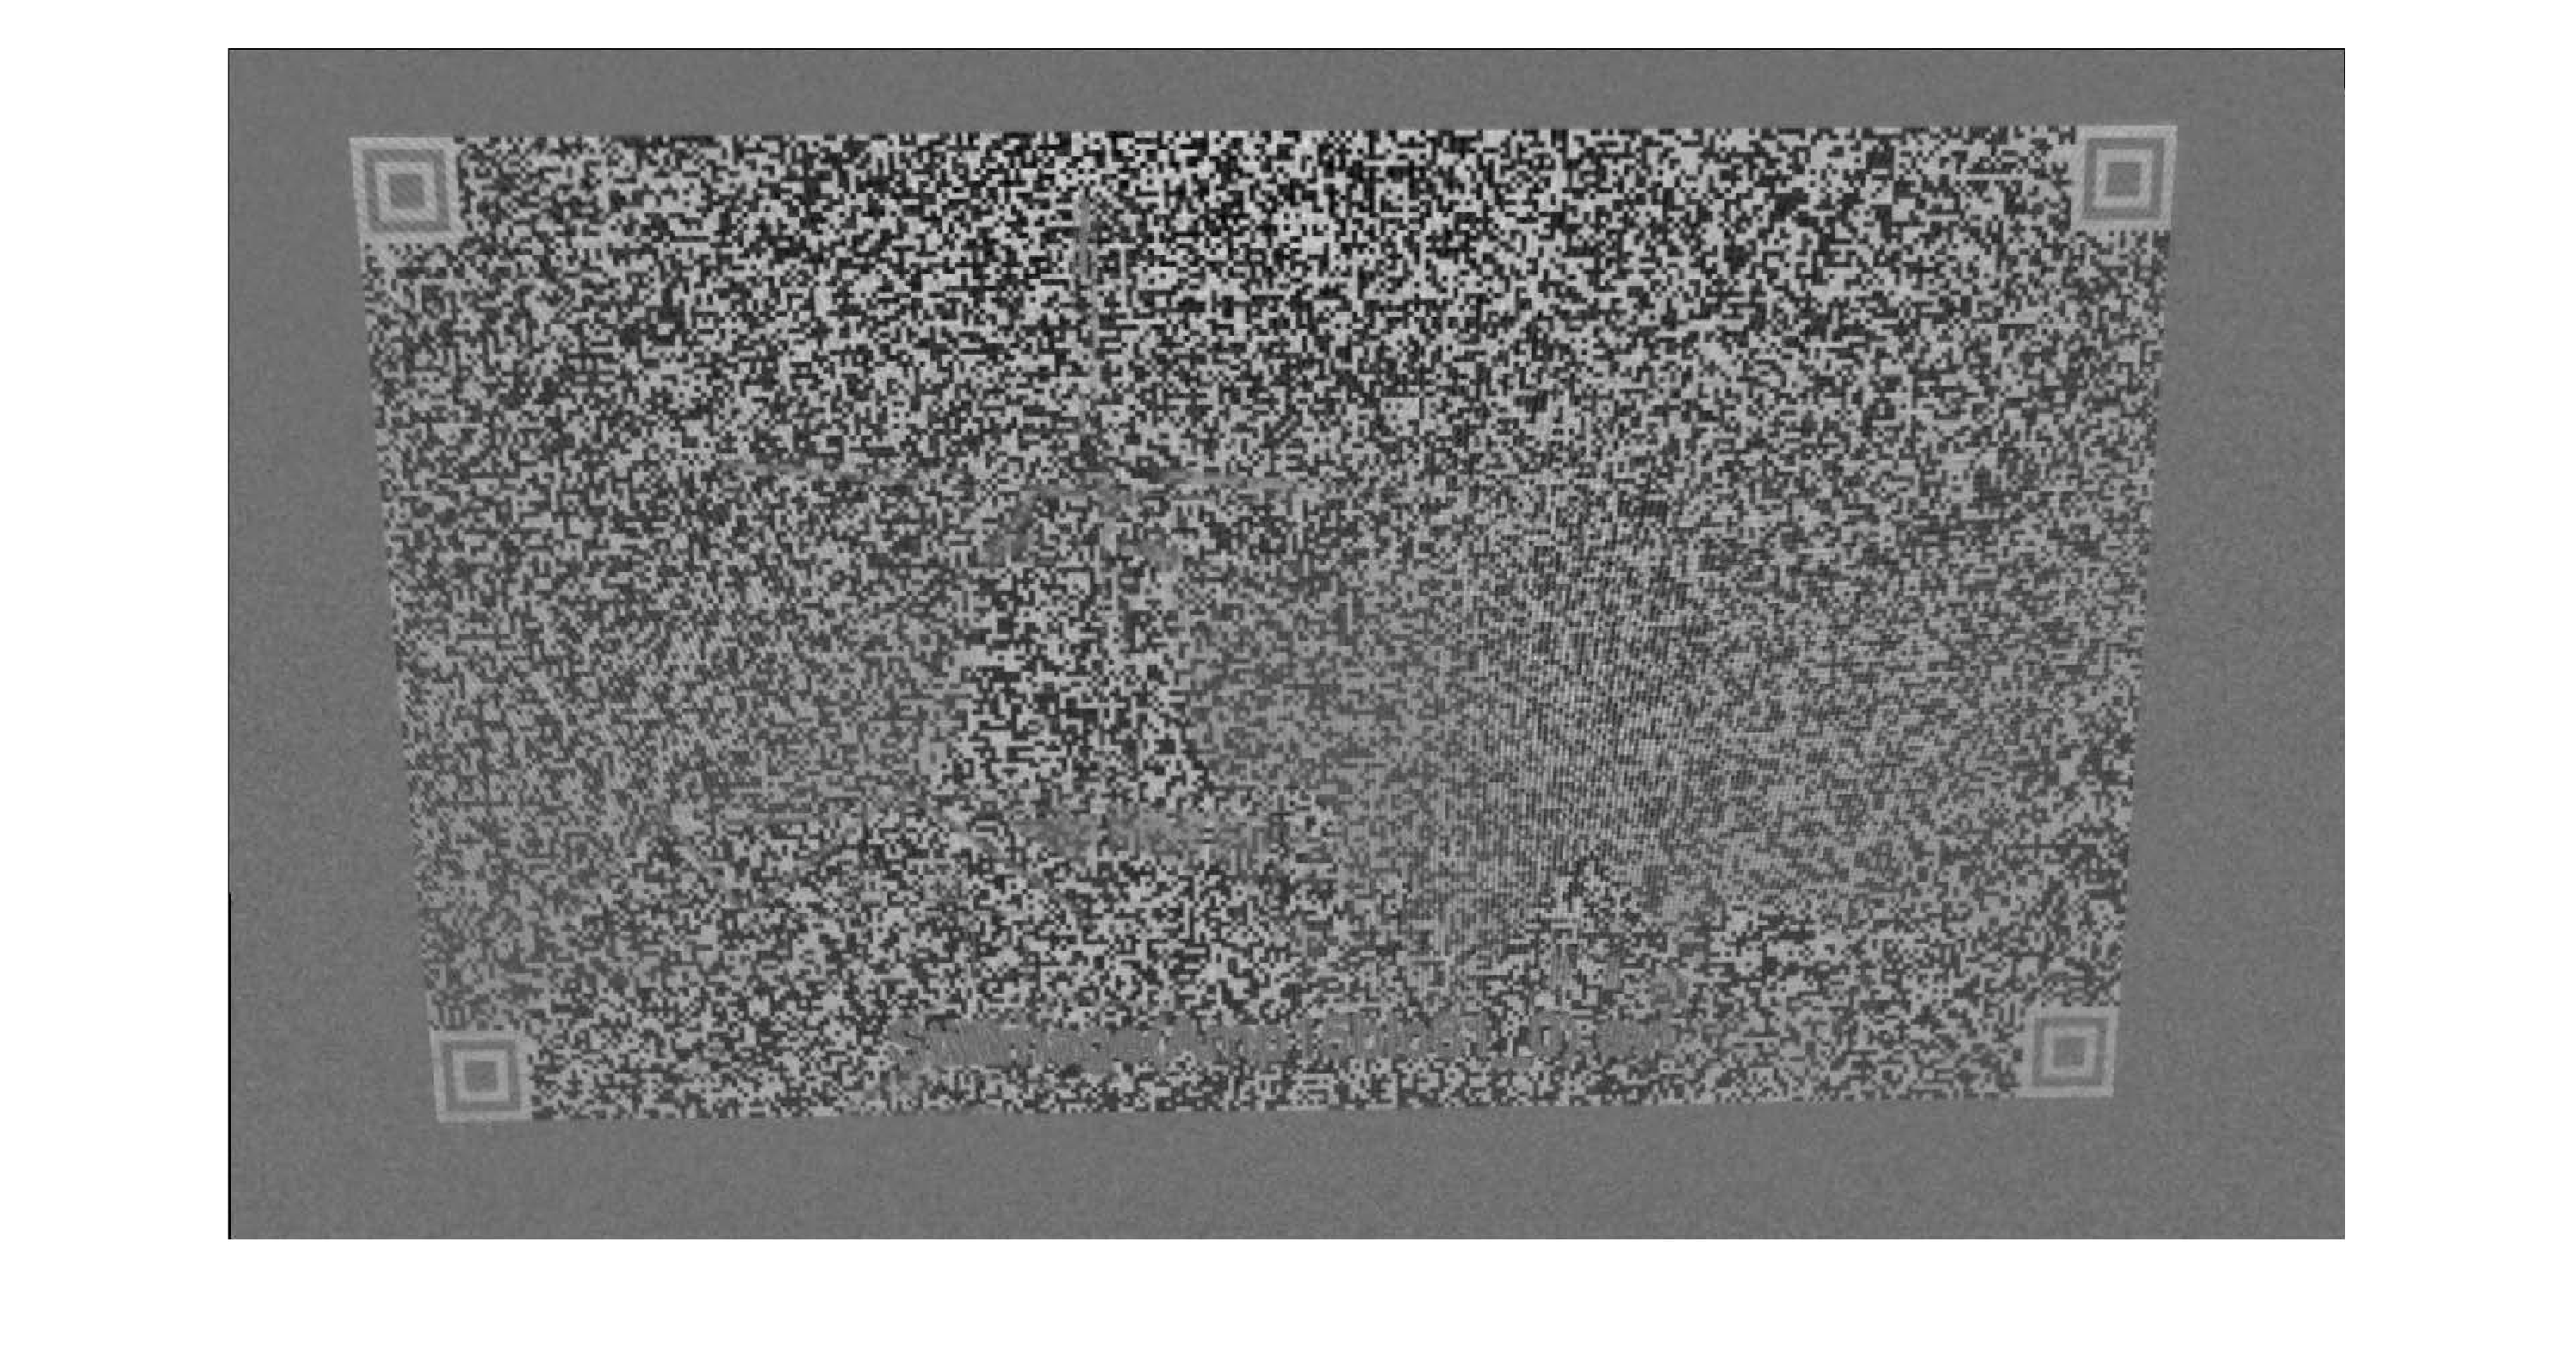
\includegraphics[scale=0.12]{images/3_Ersteverfahren/Differenzbild/0schwarz.pdf}& Nein & 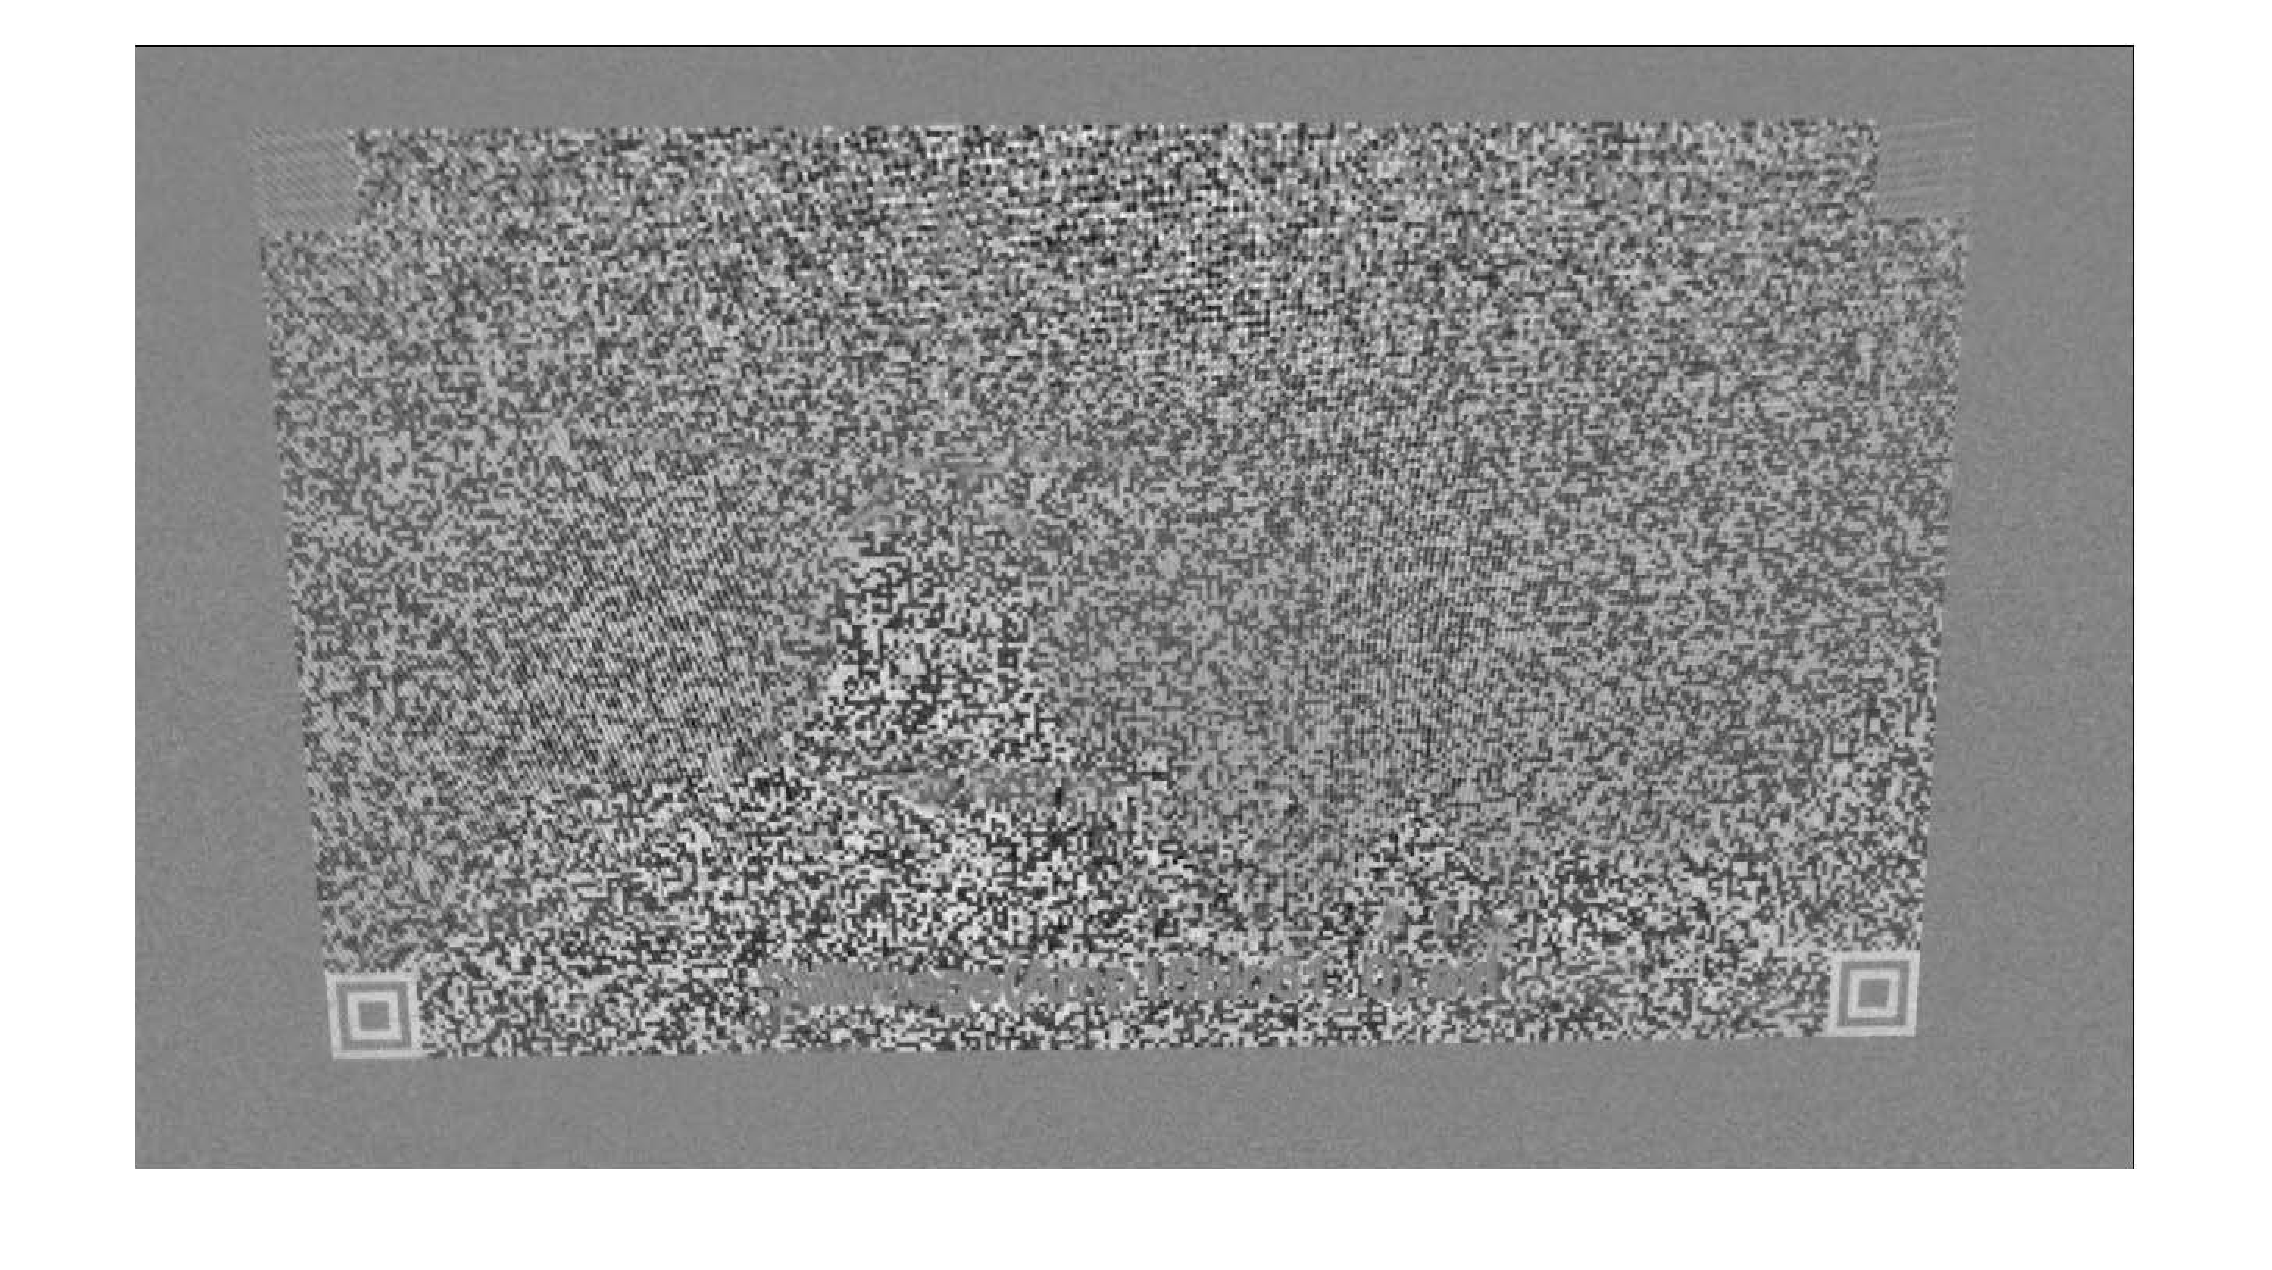
\includegraphics[scale=0.15]{images/3_Ersteverfahren/Differenzbild/1halfschwarz.pdf}\\
	Nein & 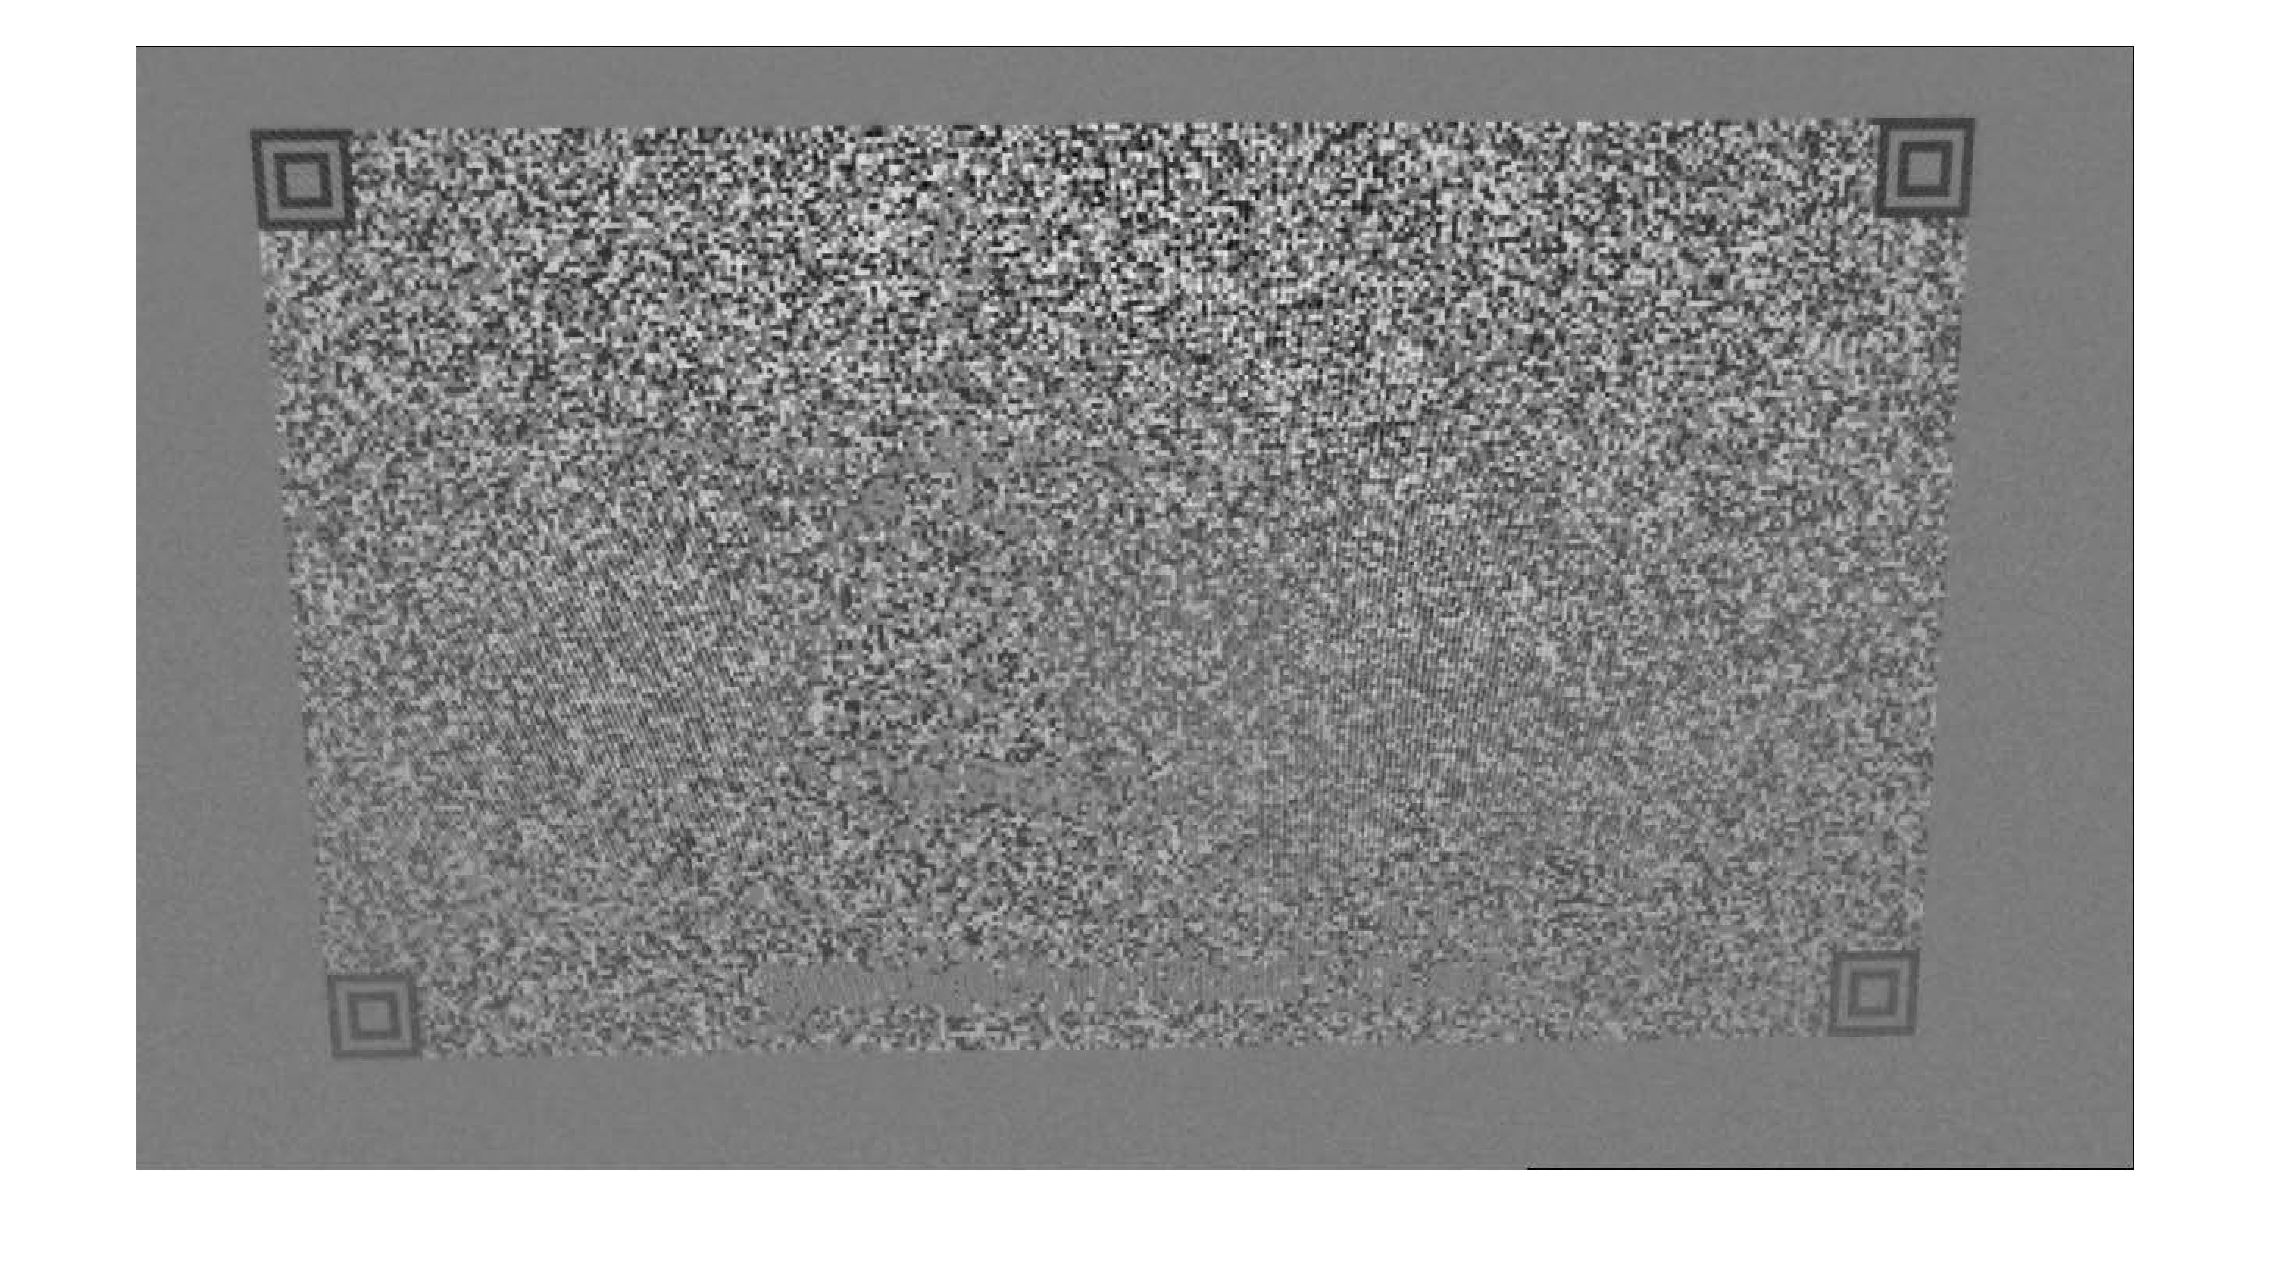
\includegraphics[scale=0.15]{images/3_Ersteverfahren/Differenzbild/2weis.pdf}& Nein & 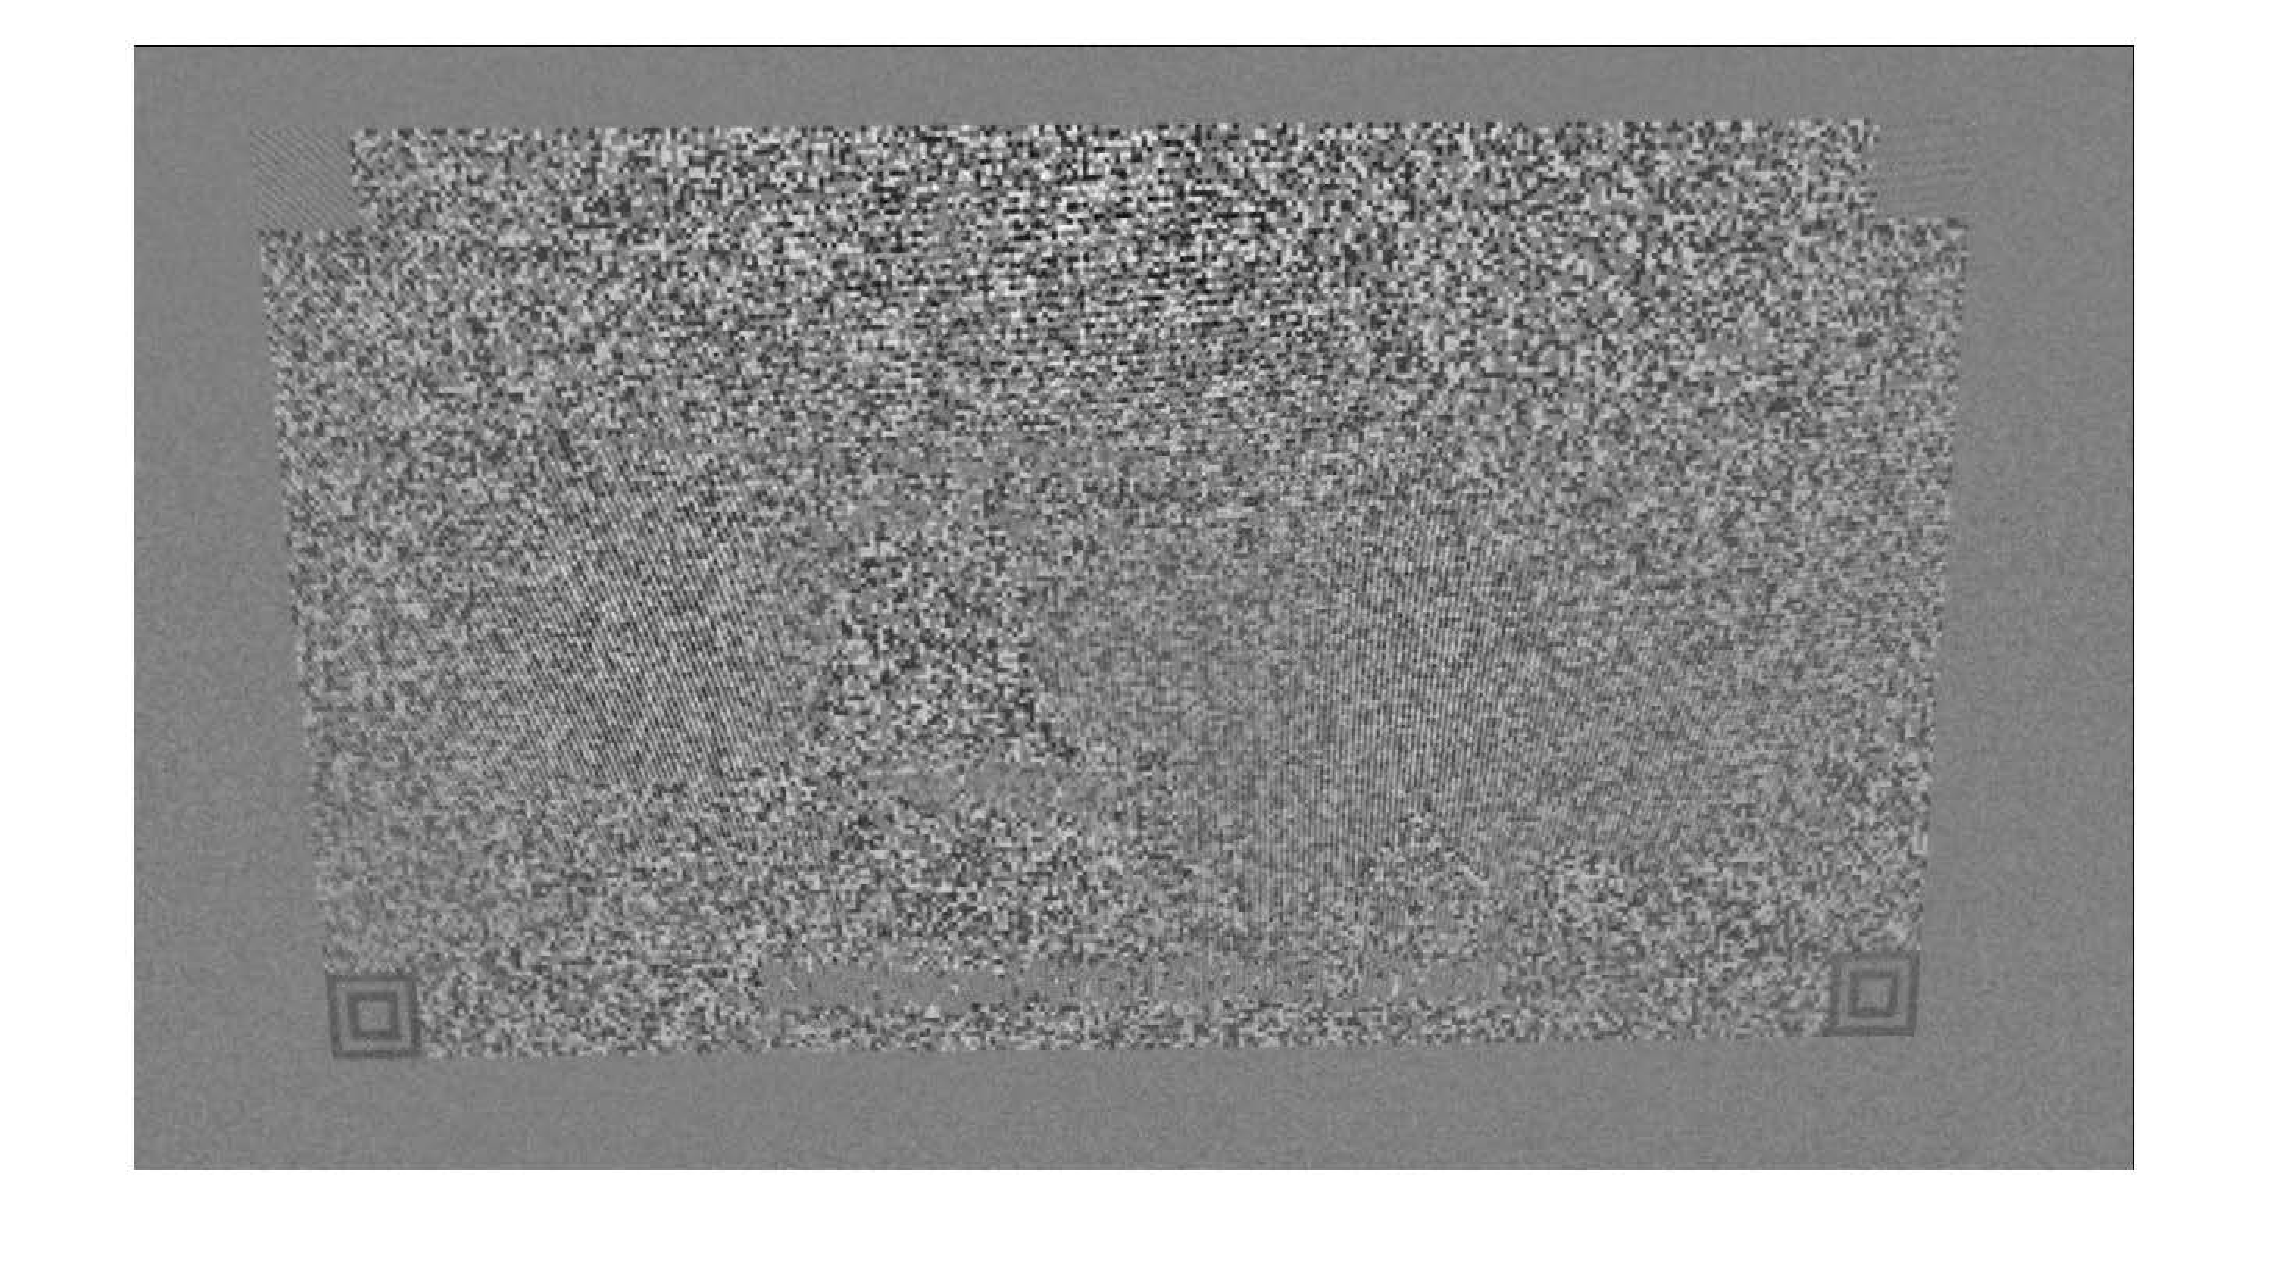
\includegraphics[scale=0.15]{images/3_Ersteverfahren/Differenzbild/3halfweis.pdf}\\
	Nein & 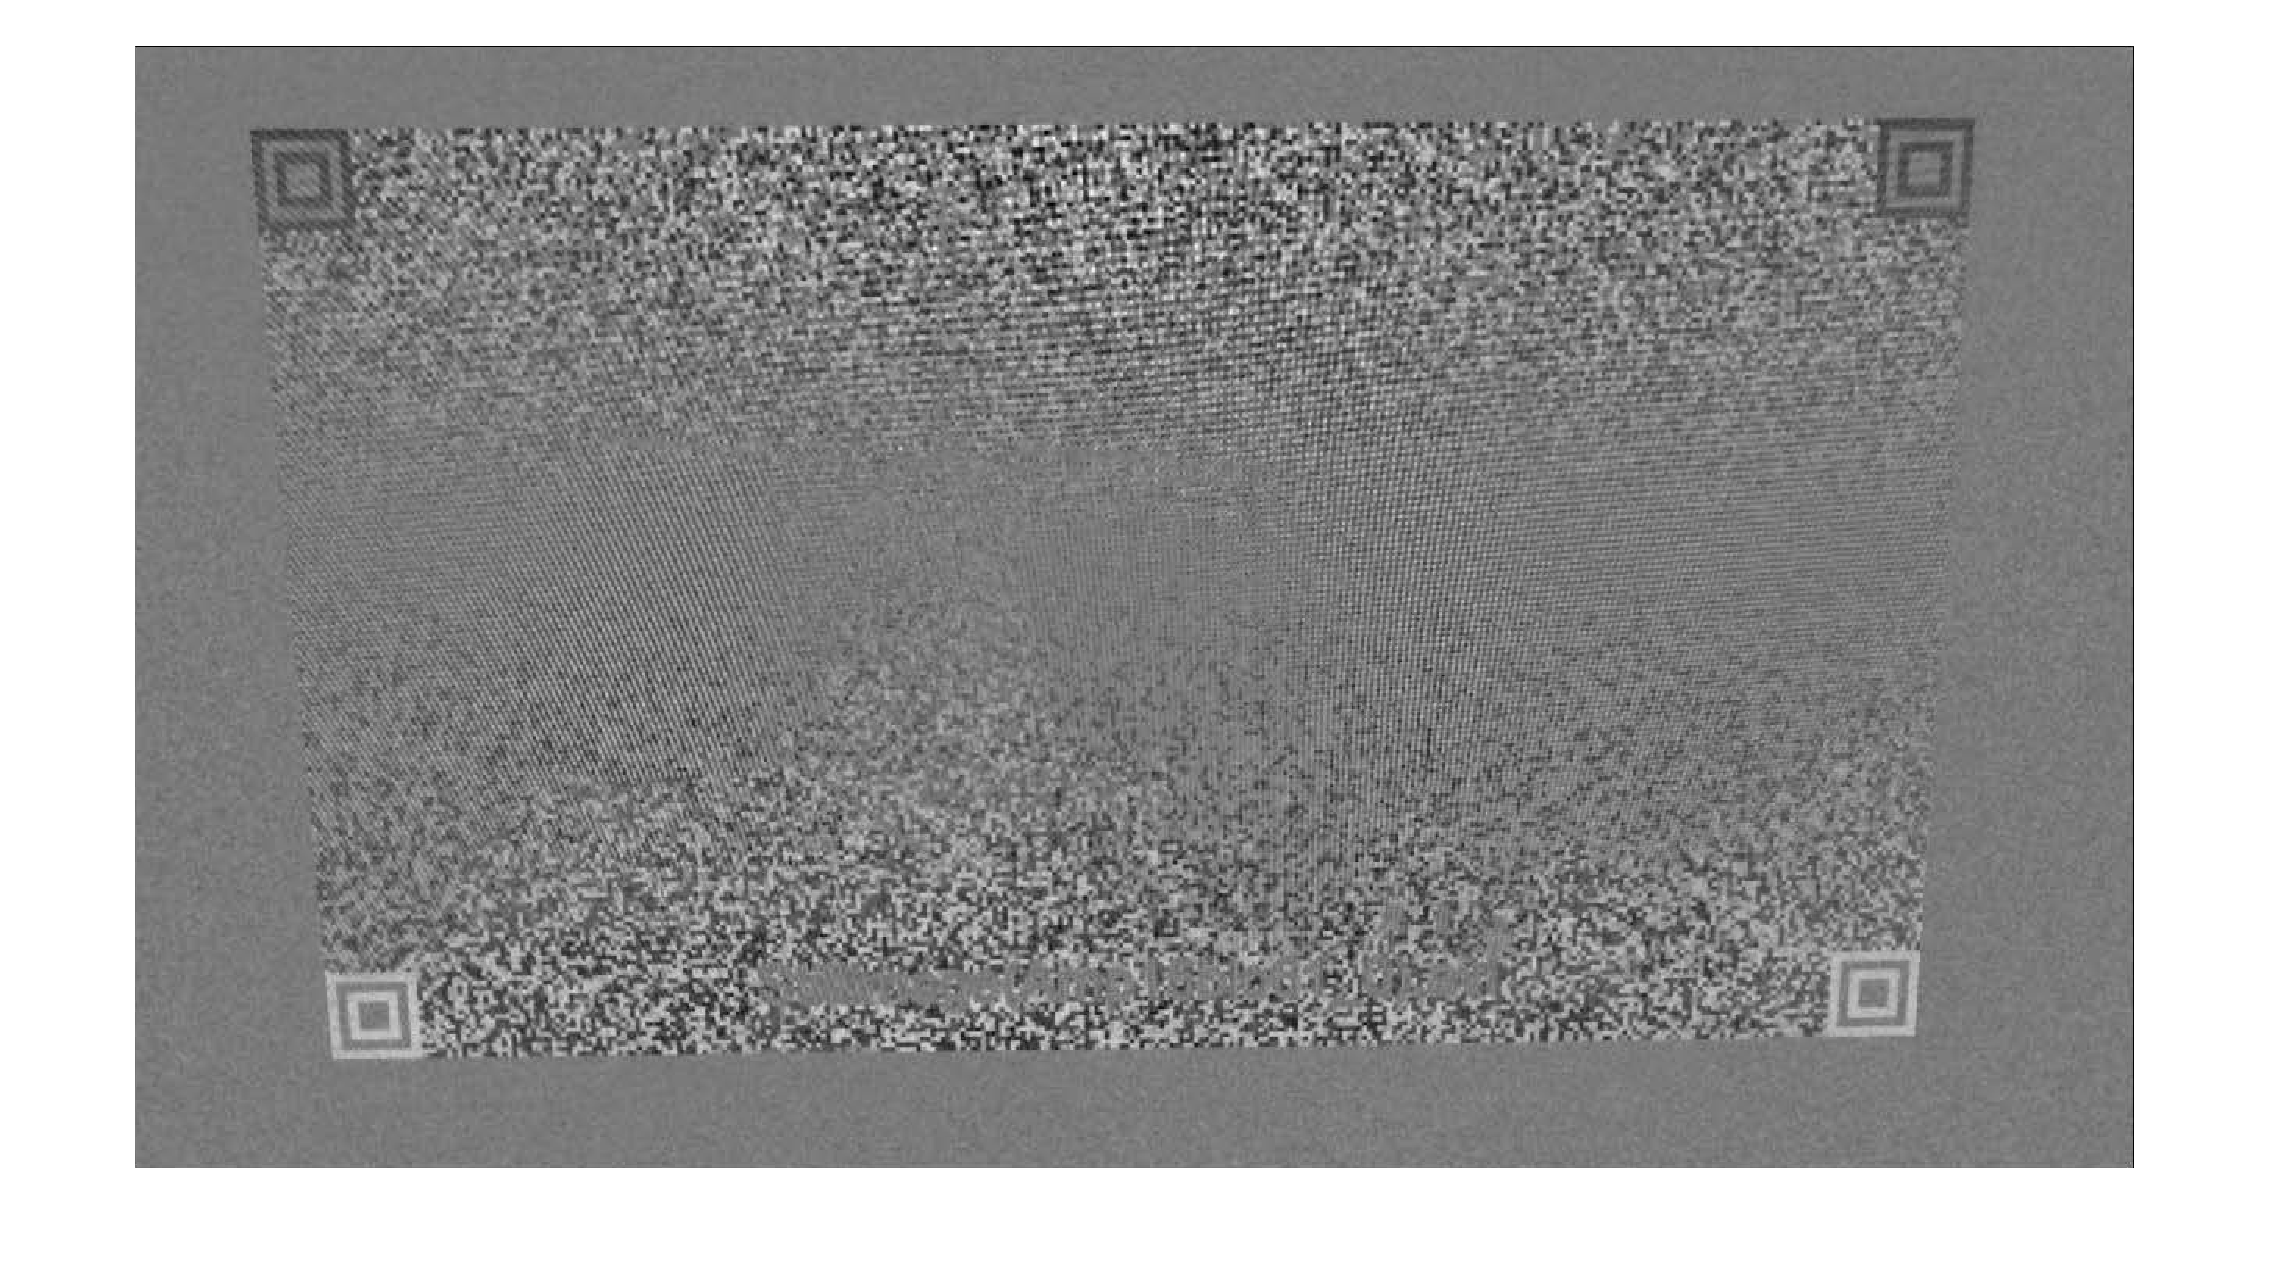
\includegraphics[scale=0.15]{images/3_Ersteverfahren/Differenzbild/4halbschwaryhalbweis.pdf}& Nein & 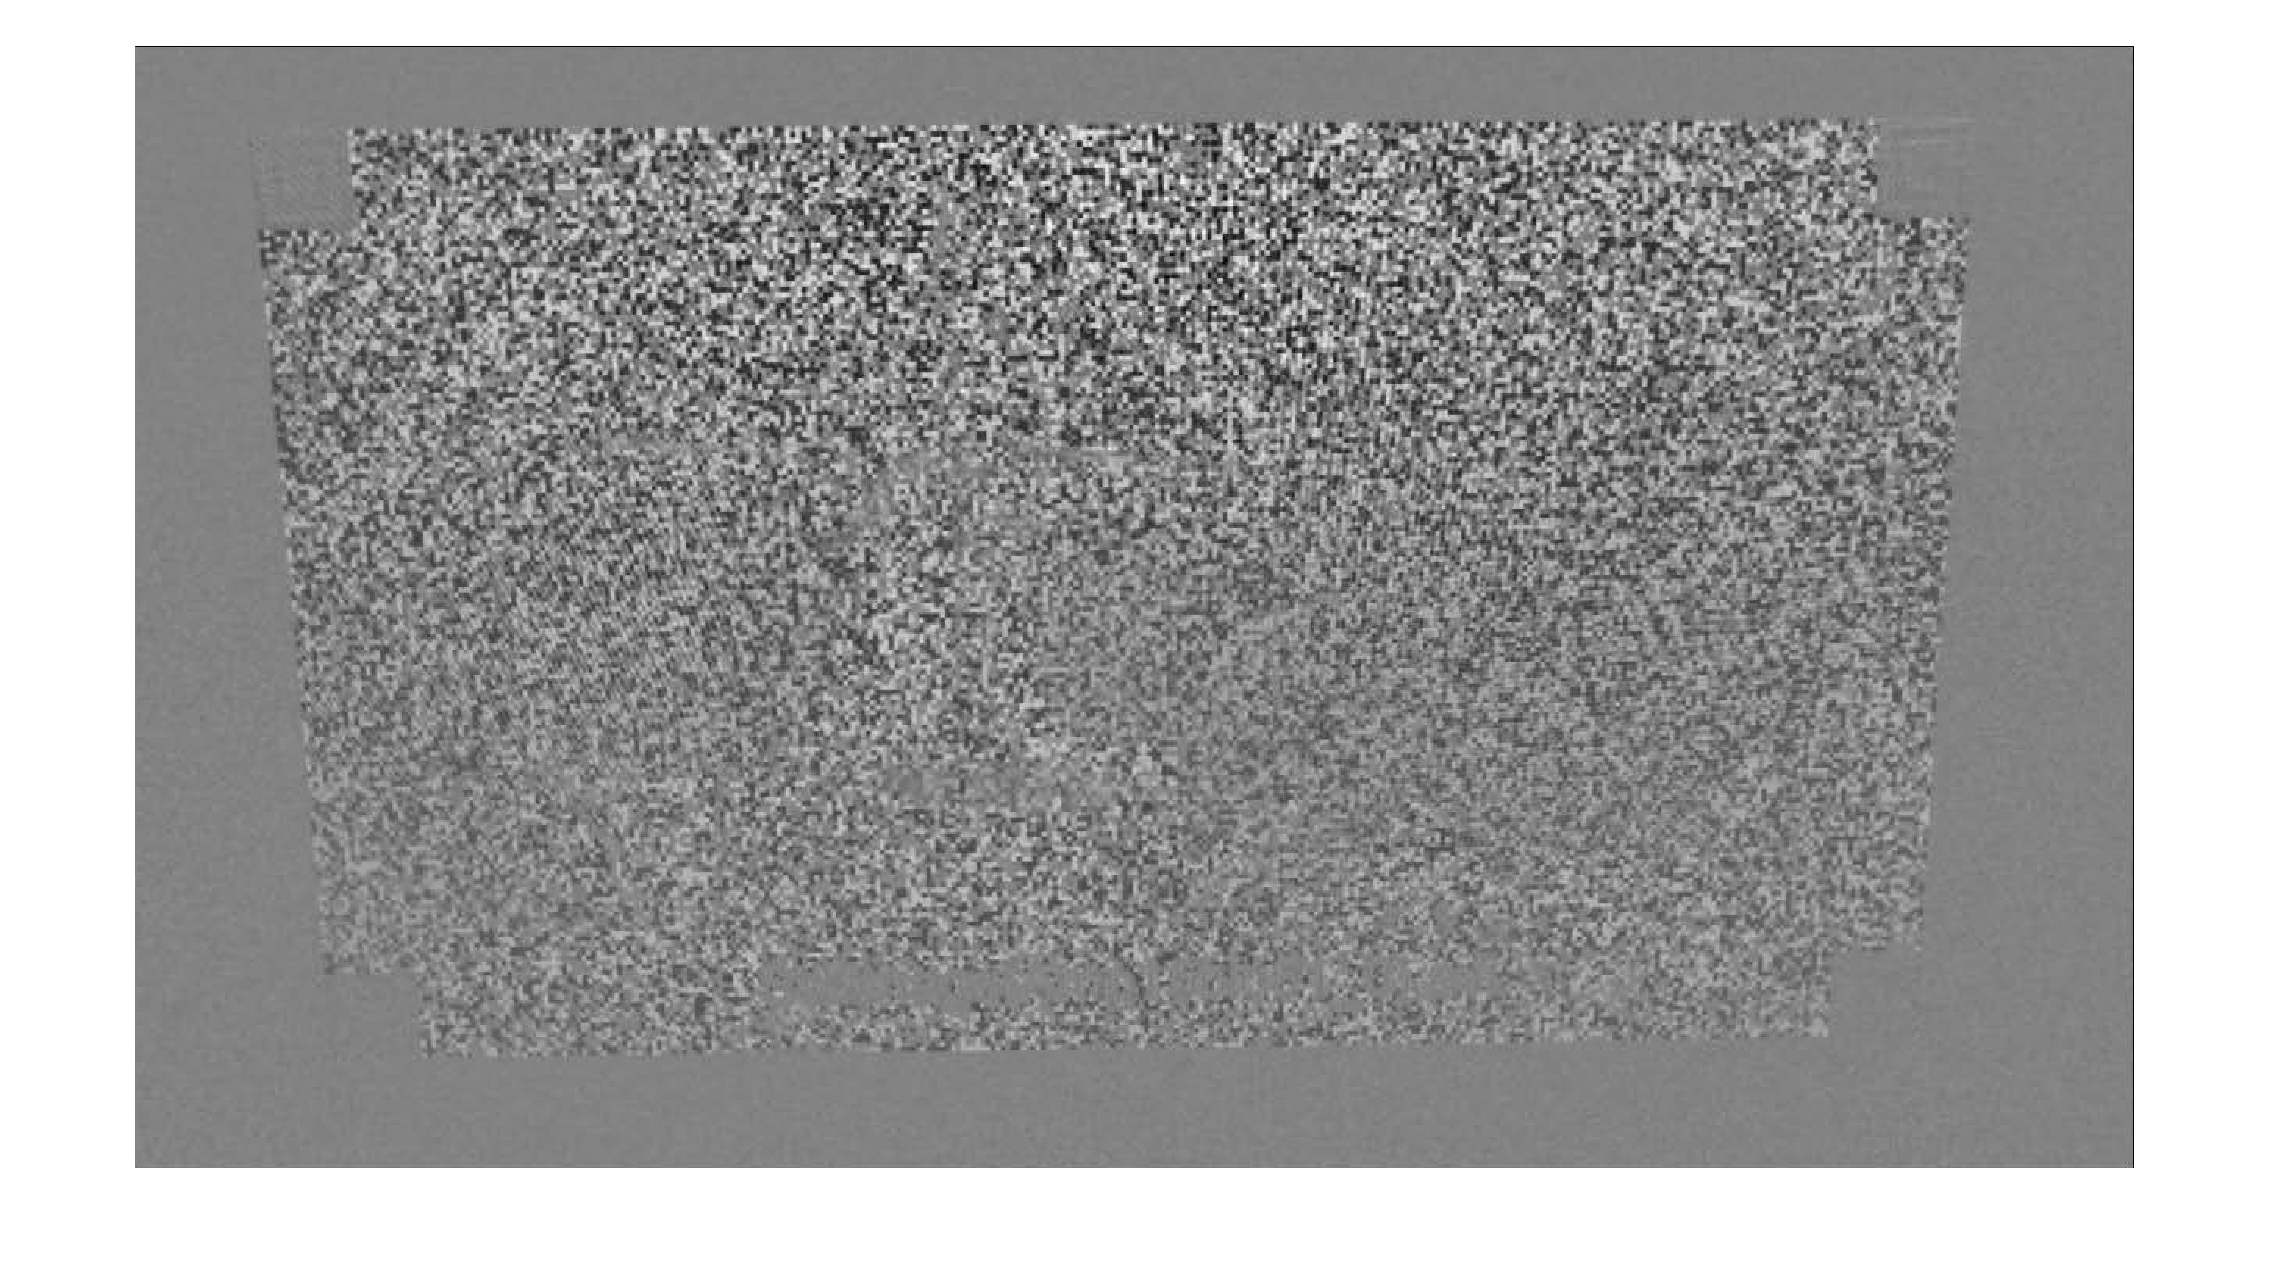
\includegraphics[scale=0.15]{images/3_Ersteverfahren/Differenzbild/5aufheben.pdf}\\

	\bottomrule
	\end{tabular}
\end{table} 


Die Struktur eines QR Musters ist in Formel 3.29 aufgeführt. Die äußerste $``1"$ Schicht ist hier ein Trennmuster und der Zentralbereich repräsentiert das QR Muster. Aufgrund der Modulationseigenschaften des \gls{david} Systems werden nur die Pixelwerte der Punkte mit dem Element $``1"$ nach der Modulation verändert. Im Vergleich dazu werden die Pixelwerte der Punkte mit dem Element $``0"$ nur gering verändert. Deswegen werden durch eine Absolutwertoperation die QR Muster als Schwarz-Weiß-Schwarz-Weiß-Schwarz Ordnung dargestellt. Dies ist die erwartete Modellstruktur die im nächsten Schritt operiert wird. Ein detailliertes Operieren wird im Abschnitt $ ``QR\,Muster\,Detektion" $ besprochen.

\begin{equation}
QR_{base} = \begin{bmatrix}
    1 &1 &1 &1 &1 &1 &1 &1 &1 \\
    1 &0 &0 &0 &0 &0 &0 &0 &1 \\
    1 &0 &1 &1 &1 &1 &1 &0 &1 \\ 
    1 &0 &1 &0 &0 &0 &1 &0 &1 \\ 
    1 &0 &1 &0 &0 &0 &1 &0 &1 \\ 
    1 &0 &1 &0 &0 &0 &1 &0 &1 \\ 
    1 &0 &1 &1 &1 &1 &1 &0 &1 \\ 
    1 &0 &0 &0 &0 &0 &0 &0 &1 \\ 
    1 &1 &1 &1 &1 &1 &1 &1 &1 \\ 
\end{bmatrix}
\end{equation}

Als nächstes wird der Begriff $``Energie"$ vorgestellt. Auf numerischer Ebene beschreibt dieser den Mittelwert des quadrierten Pixelwertes des Bildes. Es ist bekannt, dass die Pixelwerte in dem Gebiet rund um den Modulationsbereich sich durch Subtraktion der beiden Frames gegeneinander aufheben. In diesem Gebiet werden die Pixelwerte nur vom Rauschen beeinflußt und haben deshalb einen sehr kleinen Wert. Im Vergleich dazu betragen die Pixelwerte im Modulationbereich einen relativ großen Wert $\pm2A$, hier ist A die Modulationsamplitude des Systems. Der Einfluss von Zeitsynchronisation gleicht die Pixelwerte in einigen Teilen des Modulationsbereichs aufgrund von Synchronisation aus, und zwar durch aufheben der $ ``Energie" $. Die Größe der $``Energie"$ hängt hauptsächlich von den Pixelwerten im Modulationsbereich ab. Je größer die Pixelwerte sind, desto höher die $``Energie"$ des Bildes, und desto klarer kann das QR Muster werden. Gemäß dieser Regel wird die $``Energie"$ jedes Differenzbildes berechnet und in absteigender Reihenfolge angeordnet. Um die folgende Detektion zu vereinfachen, werden die ersten paar Bilder hinzugefügt. Dann wird ein zu detektierende Bilder erhaltet. %Aus dem Experiment hat bewiesen, dass es ausreicht die ersten drei Bilder zu nehmen.

Die Formel der $``Energie"$ wird in Gleichung 3.30 dargestellt. Hier repräsentiert $ m,n $ die Anzahl der Zeilen und Spalten der Matrix. $diff(i,j)$ ist der Pixelwert des Punkts in der m-ten Zeile und n-ten Spalte der Matrix.

\begin{equation}
Energie = \frac{1}{m \times n} \sum_{i=1}^m \sum_{j=1}^n diff^2(i,j) 
\end{equation}

Es folgen die detaillierten Schritte dieses Algorithmus:

\begin{enumerate}
	\item Wahl zwei beliebiger Bilder und Subtraktion dieser Bilder um das Differenzbild zu erhalten.
	\item Berechnung der Energie durch eine Absolutoperation.
	\item Sortierung in absteigender Reihenfolge und Auswahl einiger Bilder.
	\item Addition der gewählten Differenzbilder um ein zu detektierendes Bild zu erhalten.
\end{enumerate}

Dazu, das passende Flussdiagramm in Abbildung \ref{fig:DifferenzbildFlussigdiagramm}.
\begin{figure}[H]
 \centering 
 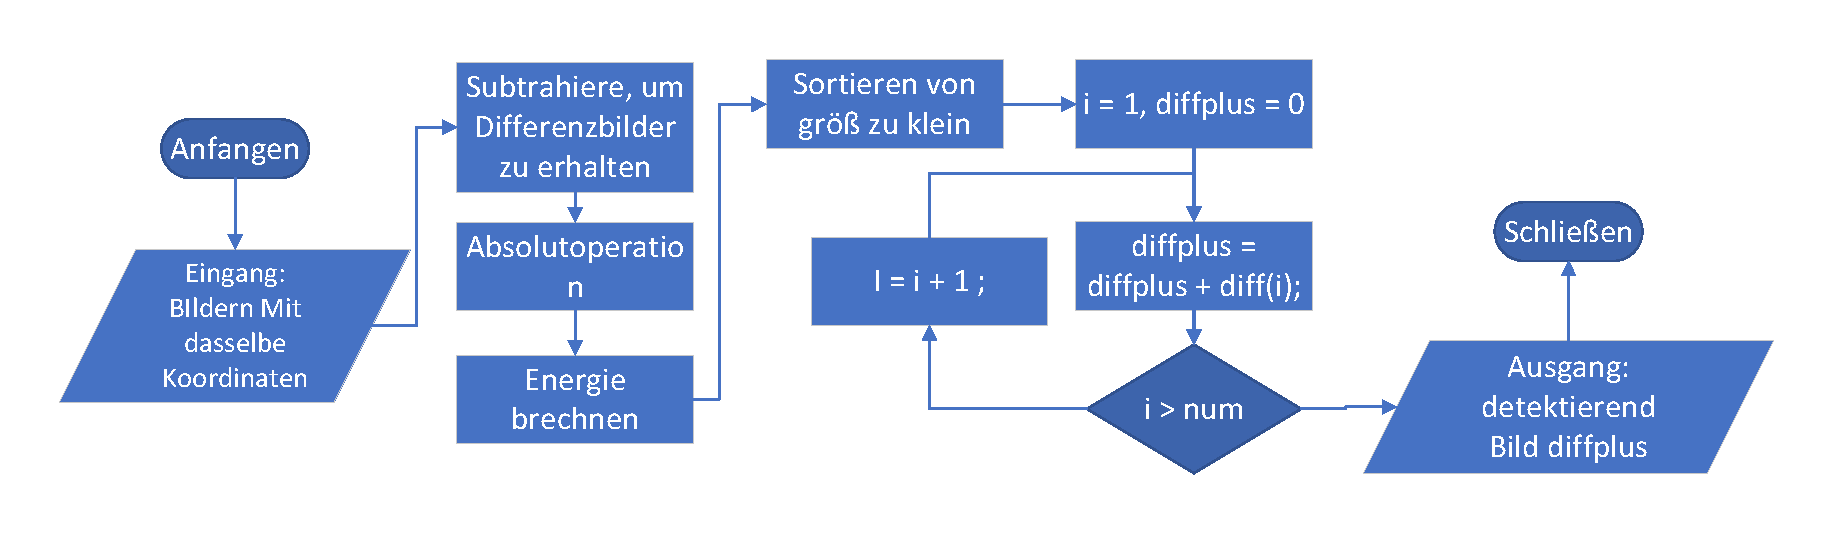
\includegraphics[keepaspectratio,width=1.1\textwidth]{images/3_Ersteverfahren/Differenzbild/Differenzbildflussigdiagramm.pdf}
 \caption{Differenzbild Flussdiagramm}
 \label{fig:DifferenzbildFlussigdiagramm}
\end{figure} 

Ein Beispiel für ein zu detektierendes Bild wird in Abbildung \ref{fig:EindetektiertesBild} vorgeführt. Aus der Abbildung ist ersichtlich, dass der Modulationsbereich besser dargestellt ist und an den vier Ecken des Bereichs ein eindeutiges QR Muster vorhanden ist. Als nächstes wird die Bildverarbeitung vorgestellt.

\begin{figure}[H]
 \centering 
 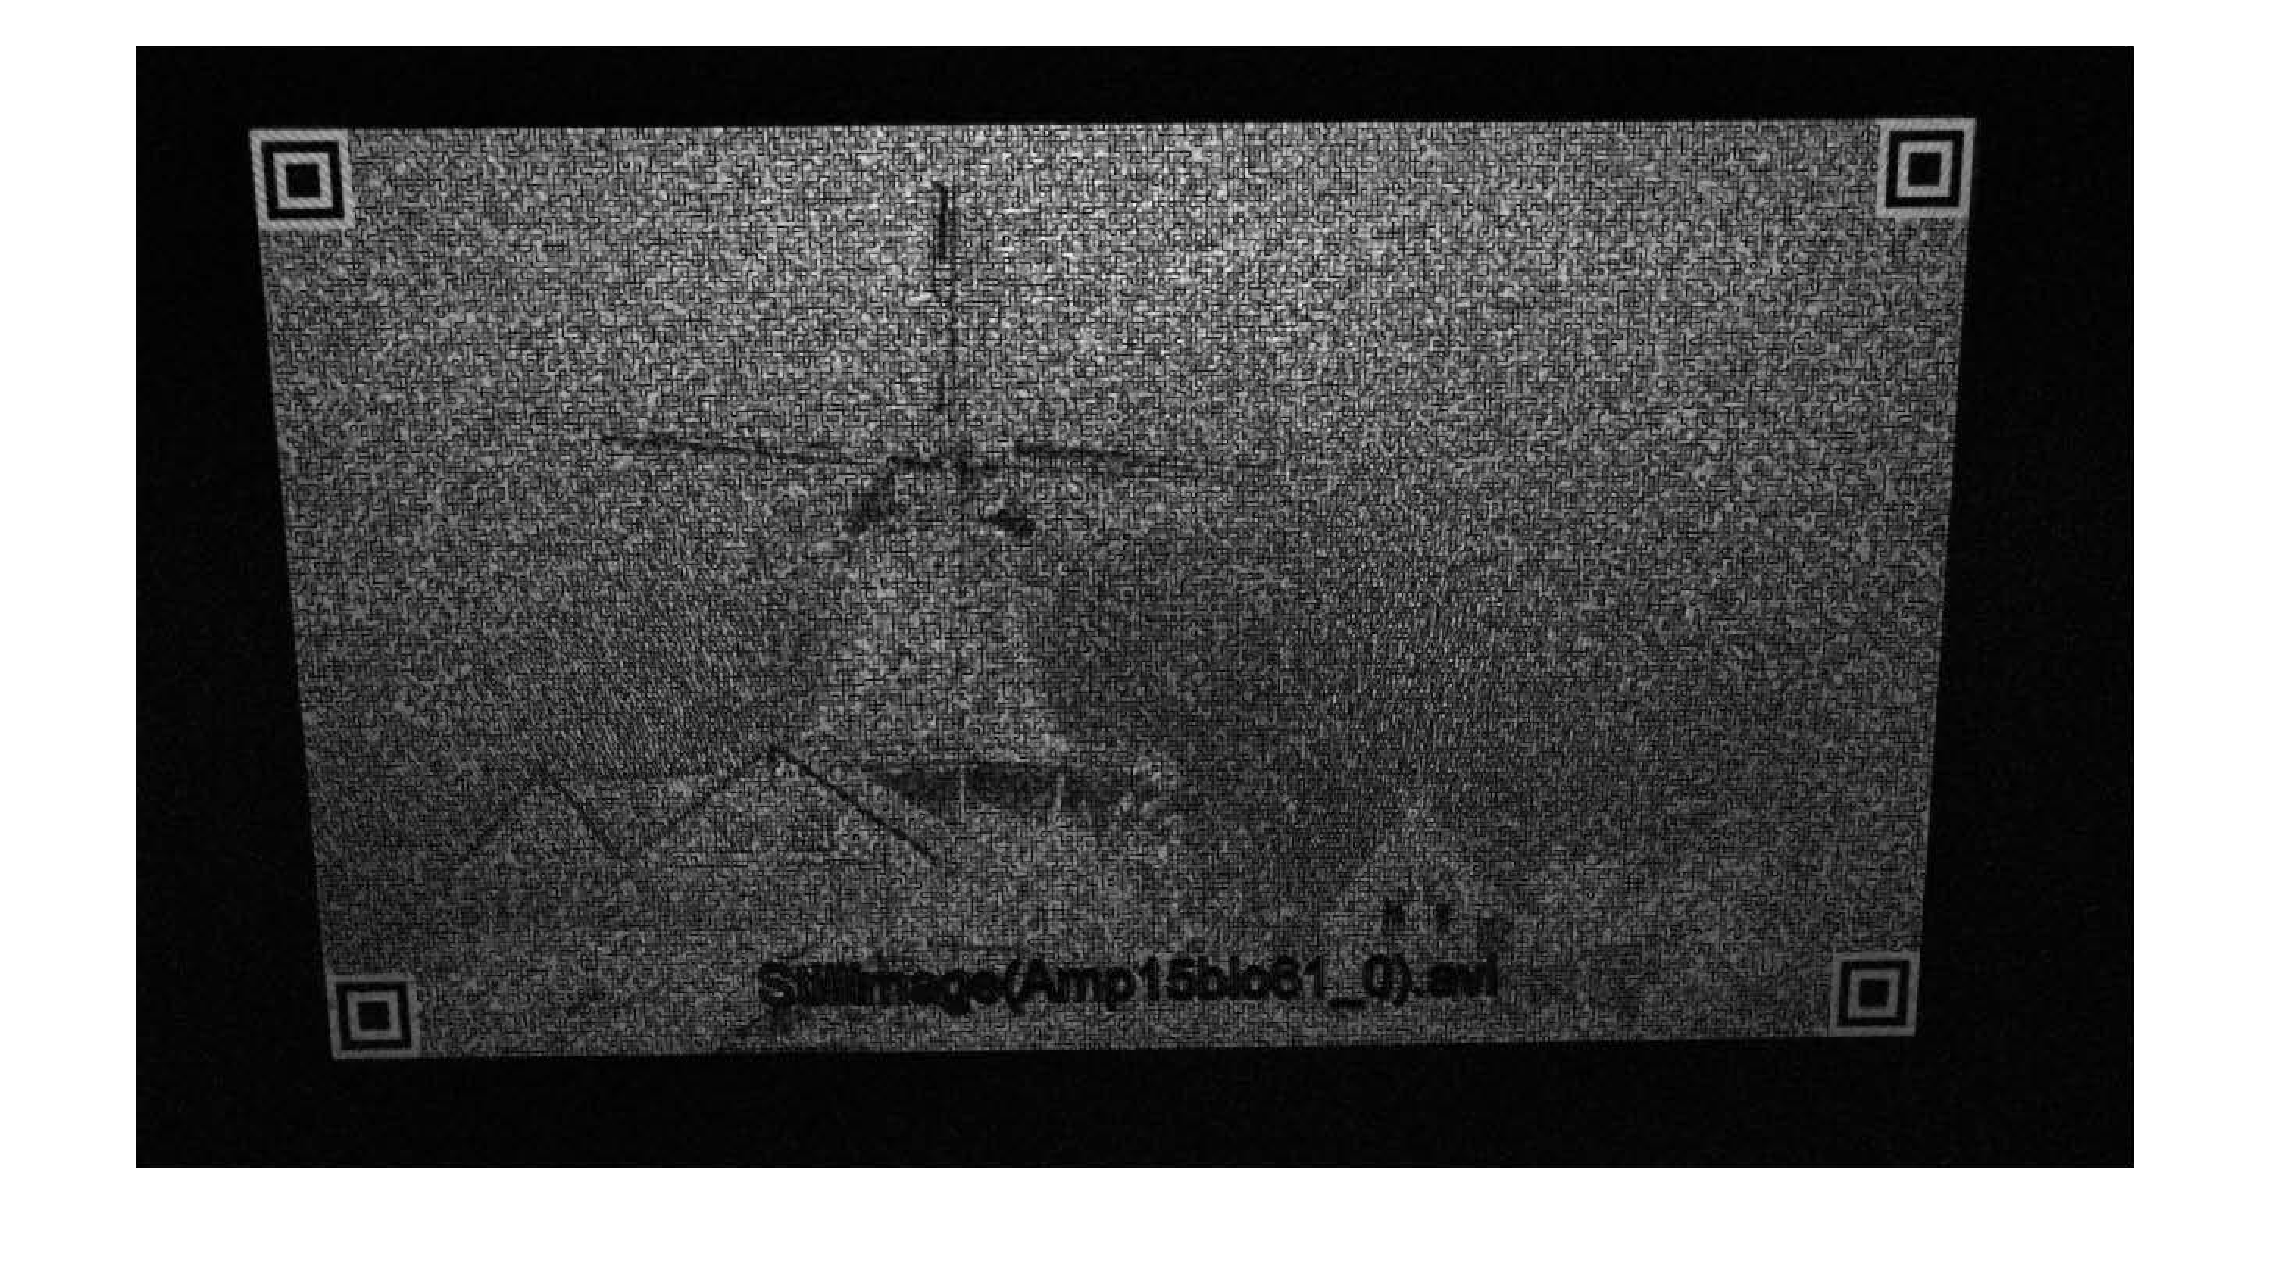
\includegraphics[keepaspectratio,width=0.8\textwidth]{images/3_Ersteverfahren/Differenzbild/diffplus.pdf}
 \caption{Ein zu detektierendes Bild}
 \label{fig:EindetektiertesBild}
\end{figure} 


\section{Bildverarbeitung} 
Durch die Differnzbild-Optimierung, wird ein zu detektierendes Bild erhalten. Abbildung \ref{fig:EindetektiertesBild} ist noch ein Graustufenbild und muss noch einiger Bildverarbeitung unterzogen werden. Dadurch können kleine Punkte und Lücken, die durch Rauschen und Fehler verursacht wurden, entfernt werden um die nachfolgende Detektion zu erleichtern. Der detaillierte Inhalt der Bildverarbeitung wurde in der anderen Methode aufgeführt. Es folgt eine kurze Beschreibung. 

\textbf{Bild Binarisierung}

Für die Schwellenwertbildung und das Erstellen eines Binärbildes wurde eine Funktion namens $ ``imbinarize" $ in Matlab verwendet. Dieser Funktion wird das Bild übergeben, damit es einen anpassungsfähigen Schwellwert generiert um das Schwarz-Weiß-Bild zu erstellen. Dies ist ausreichend für die QR Muster Detektion, weil es nur schwarze und weiße Module enthält, die binär 1 bzw. 0 sind. 

%\textbf{Medianfilter}

%Der Grund für das Median-Filtern ist, dass manchmal beim Prozess der Binarisierung aus einem Bild Effekte wie Salz- und Pfeffergeräusche entstehen können. Um diesen Fehler zu vermeiden, ist Median Filterung eine zuverlässige Methode. Eine Funktion namens $ ``medfilt2" $ wurde in Matlab verwendet. Zur Verbesserung der Ergebnisse können auch die verschiedenen Fenstergrößen für die Matlab-Funktion verwendet werden.

\textbf{Morphologie}

Mit öffnenden und schließenden Filtern können die Lücken zwischen Blöcken und die Punkte vom Rauschen stark reduziert werden, was das binär Bild zu einer guten Interpretation des QR Musters macht. 

\section{QR-Muster-Detektion} 

Nach der Bildverarbeitung wird nun die QR Muster Detektion ausgeführt. Das Ziel einer QR Muster Detektion ist, das Zentrum des Musters im Bild zu lokalisieren um dadurch das Bild zu rekonstruieren. Abbildung \ref{fig:QRPattern} zeigt die geometrische Struktur eines QR Musters. An jeder Ecke des Modulartionsbereichs gibt es ein solches QR Muster.

\begin{figure}[H]
 \centering 
 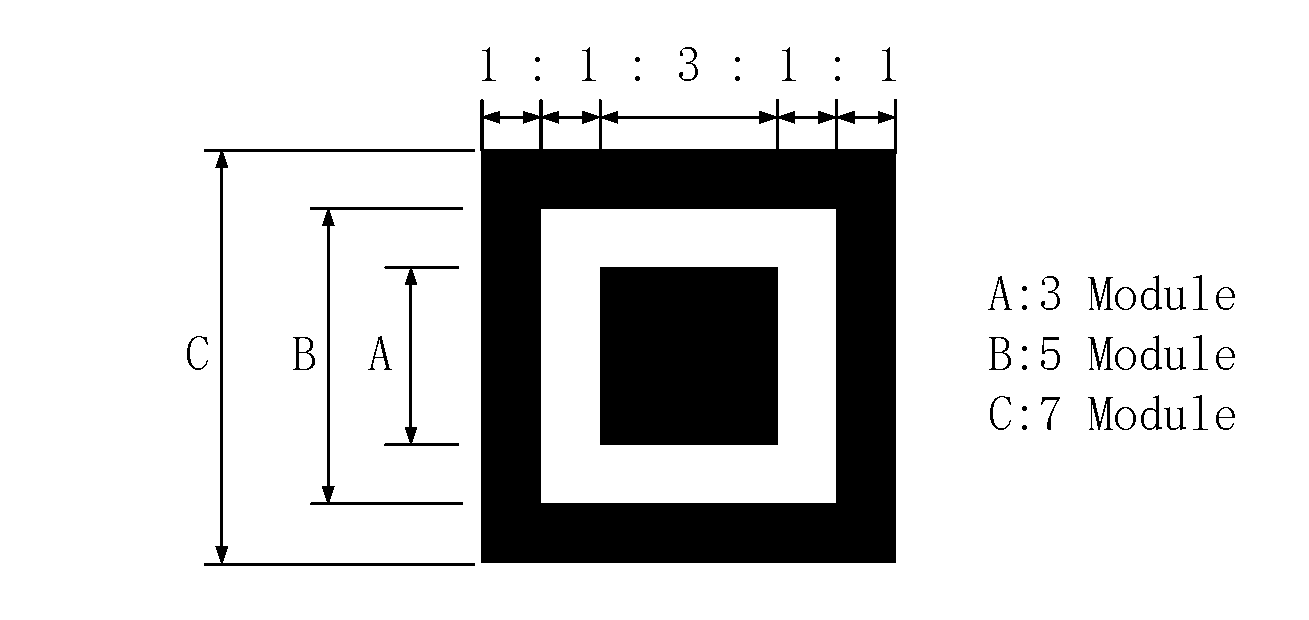
\includegraphics[keepaspectratio,width=0.9\textwidth]{images/3_Ersteverfahren/QRMuster/QRPattern.pdf}
 \caption{QR Muster}
 \label{fig:QRPattern}
\end{figure}

Aus der geometrischen Sicht kann jedes Muster als drei konzentrische Quadrate betrachtet werden und besteht aus einem schwarzen (dunklen) $7 \times 7$ Modul, einem weißen (hellen) $5 \times 5$ Modul und schließlich einem schwarzen (dunklen) $3 \times 3$ Modul. Von Kenntnissen der Geometrie ist bekannt, dass in jeder Richtung das Breiteverhältnis der alternativen Schwarz- und Weißmodul in einem Muster die Beziehung $1:1:3:1:1$ existiert, wie es in Abbildung \ref{fig:QRPatternRatio} vorgeführt ist. Diese wichtige Eigenschaft hilft uns, die Positionen der QR Muster zu finden. In der Praxis gibt es rund um die Muster noch ein Trennmuster, das ein Funktionsmuster aller weißen (hellen) Module (ein Modul breit) ist. Es dient als eine Grenze zwischen den Mustern und dem Datenbereich, um die Verwechslung zwischen Muster und Daten zu vermeiden.
 
 \begin{figure}[H]
 \centering 
 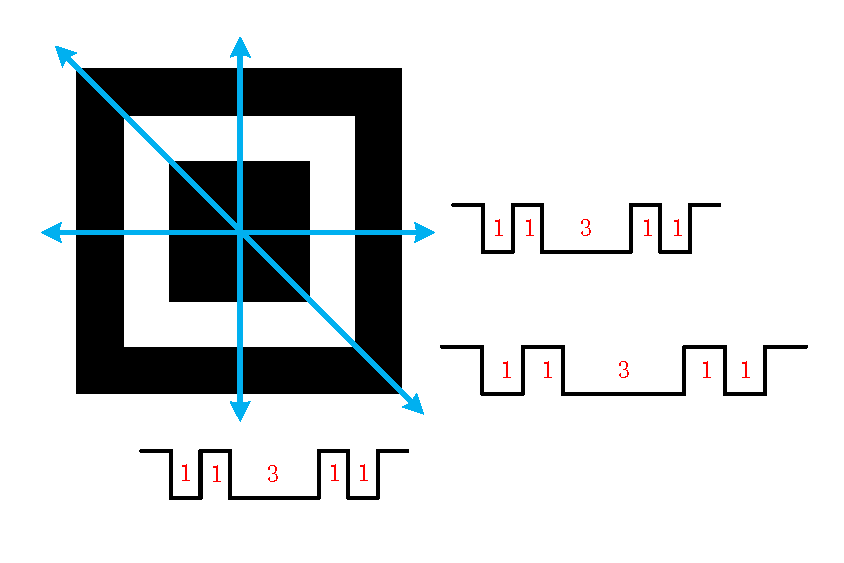
\includegraphics[keepaspectratio,width=0.7\textwidth]{images/3_Ersteverfahren/QRMuster/QP_Patternratio.pdf}
 \caption{QR Muster Ratio}
 \label{fig:QRPatternRatio}
\end{figure}

Als nächstes werden die detaillierten Schritte der Detektion aufgeführt welche mit der Funktion $ ``detectFIP" $ in Matlab implementiert wurde.

\textbf{Schritt 1:}

Zuerst wird der Berechnungsaufwand der Analyse des ganzen Bildes geschätzt, und anschließend wird der Modulationsbereich in kleine Bereiche unterteilt, die die QR Muster beinhalten.

\textbf{Schritt 2:}

Scannen jeder Zeile dieses kleinen Bereiches und Speicherung der Länge der Schwarz und Weiß Module in einen fünf Elementen Vektor. Die Länge der Module bedeutet die Anzahl aufeinanderfolgender Pixel in einer Zeile mit der gleichen Farbe. Die Speicherreihenfolge in diesem Vektor ist Schwarz-Weiß-Schwarz-Weiß-Schwarz. Es sollte hier angemerkt werden, dass das erste Element des Vektors die Anzahl der schwarzen Module enthält. 

\textbf{Schritt 3:}

Immer wenn das fünfte Element des Vektors gezählt wird, werden die Werte ausgewertet, ob das Muster nahe genug an den $1:1:3:1:1$ Verhältnissen daran ist. Wenn die Bedingung erfüllt ist, gehen zum Schritt 4. Ansonsten wird der Vektor um zwei Elemente nach links verschoben und die ersten zwei Elemente des Vektors werden entfernt. Kehren zum Schritt 2 zurück.
              

\textbf{Schritt 4:}

Die Elemente vom Vektor werden verarbeitet, um das ungefähre horizontale Zentrum zu erhalten. Eine Kreuzprüfung wird an diesem Punkt vorgenommen, welche aus den Schritten 2 und 3 besteht, der Unterschied besteht darin, dass der horizontale Scan durch einen vertikalen Scan ersetzt wird. Anschließend wird überprüft, ob ein vertikales Zentrum gefunden wurde. Wenn Ja wird eine Kreuz-Kreuzprüfung mit dem horizontalen Scan vorgenommen, um die Ergebnisse zu optimieren. Dies wird hauptsächlich benötigt, um die reale horizontale Mitte des Musters in extremen Schräglage Fällen zu lokalisieren. Nach Speicherung des potenziellen Zentrums, werden die Elemente des Vektors geleert um wieder im zweiten Schritt einen Scan zu machen. Ansonsten wird der Vektor um zwei nach links verschoben und die ersten beiden Elemente des Vektors weggeworfen. In Schritt 2, wird wiederum erneut begonnen zu scannen und zu zählen.  

\textbf{Schritt 5:}

Die Ausgabe des vorherigen Schritts wird verarbeitet. Falls mehrere potentielle Muster gefunden wurden, wird $ ``Select Best Pattern" $ verwendet, um das Beste Auszuwählen. Es sollte angemerkt werden, dass wenn die möglichen Muster nach dem Ende der Erkundung nicht gefunden wurden, ein spezielles Signal zurückgegeben wird und das System zur Schritt Differenzbild Optimierung zurückkehren wird. Die Operation besteht darin dem ursprünglichen Bild, welches aus einige Differenzbildern besteht, ein mehreres Differenzbild hinzuzufügen.
                       
\textbf{Schritt 6:}

Durch die gefundenen Muster Zentren, wird eine projektive Transformation vorgenommen, um die Ecken des Bildes zu bestimmen.


Die folgende Abbildung \ref{fig:FlussdiagrammQRMuster} zeigt ein Flussdiagramm einer Detektion für QR Muster.

\begin{figure}[htb]
 \centering 
 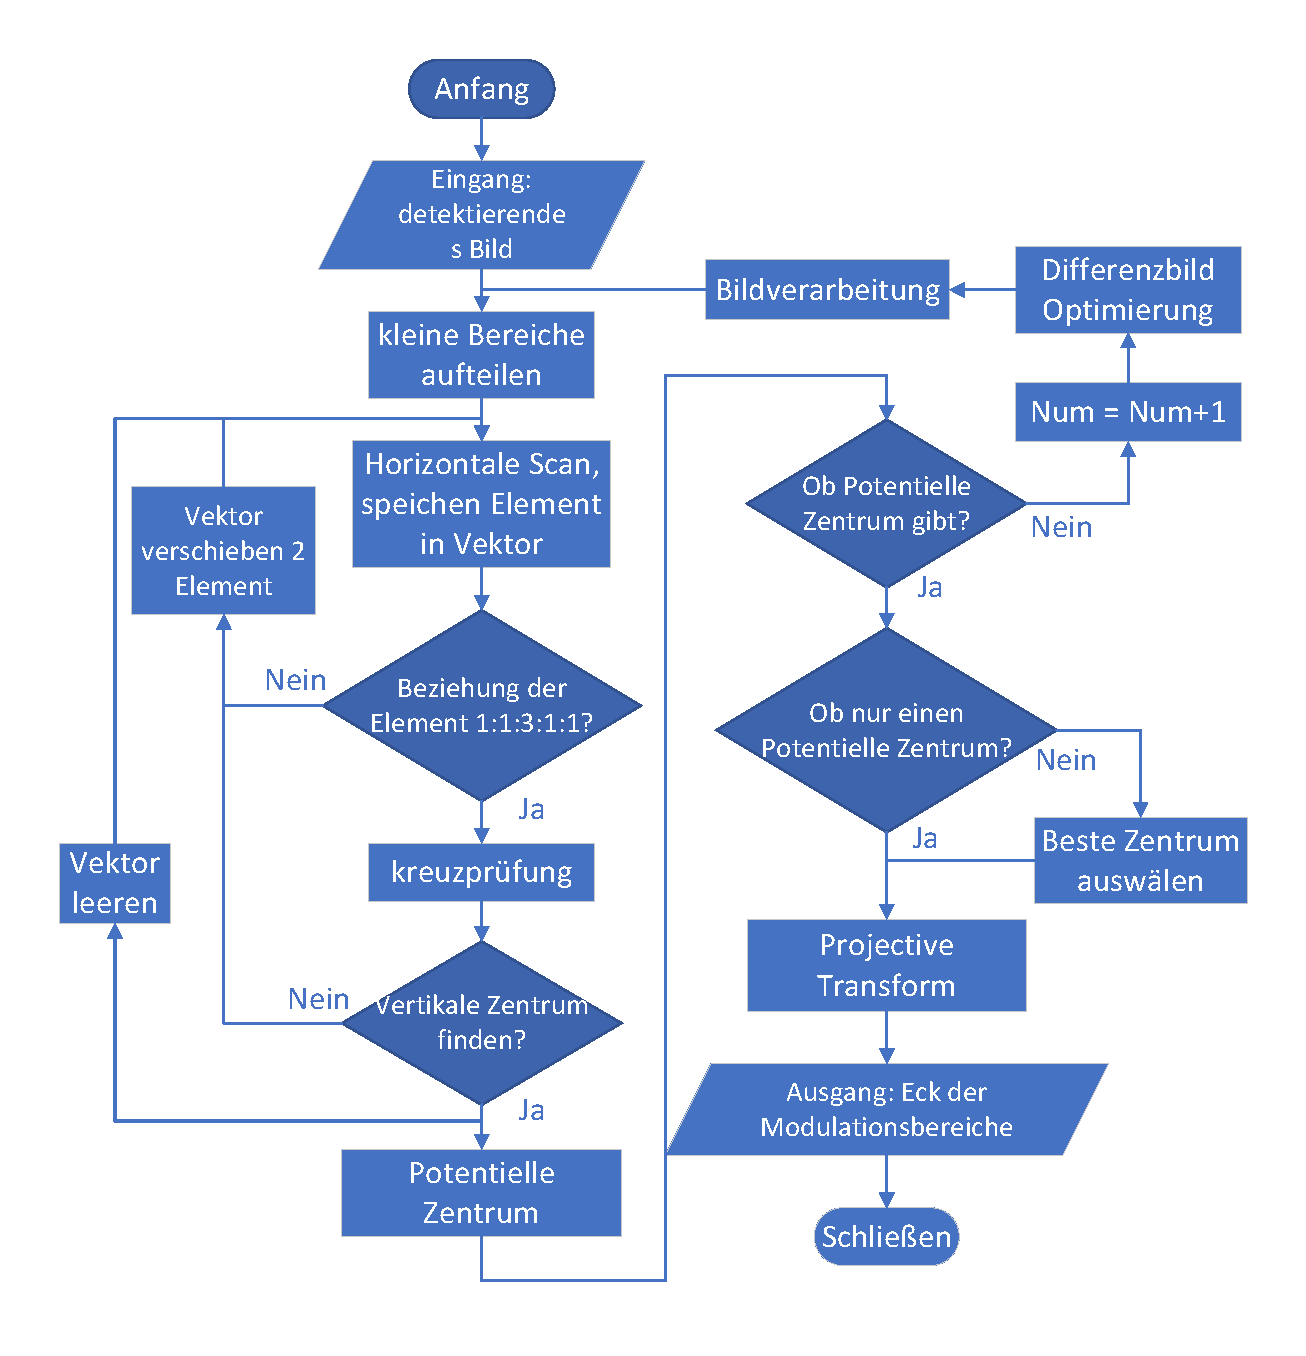
\includegraphics[keepaspectratio,width=1.0\textwidth]{images/3_Ersteverfahren/QRMuster/QR_flussdiagramm.pdf}
 \caption{Flussdiagramm der QR Muster Detektion}
 \label{fig:FlussdiagrammQRMuster}
\end{figure}

Ein Beipiel für QR Muster Detektion wird in Abbildung \ref{fig:QRMusterBeispiel} vorgeführt:

\begin{figure}[htb]
 \centering 
 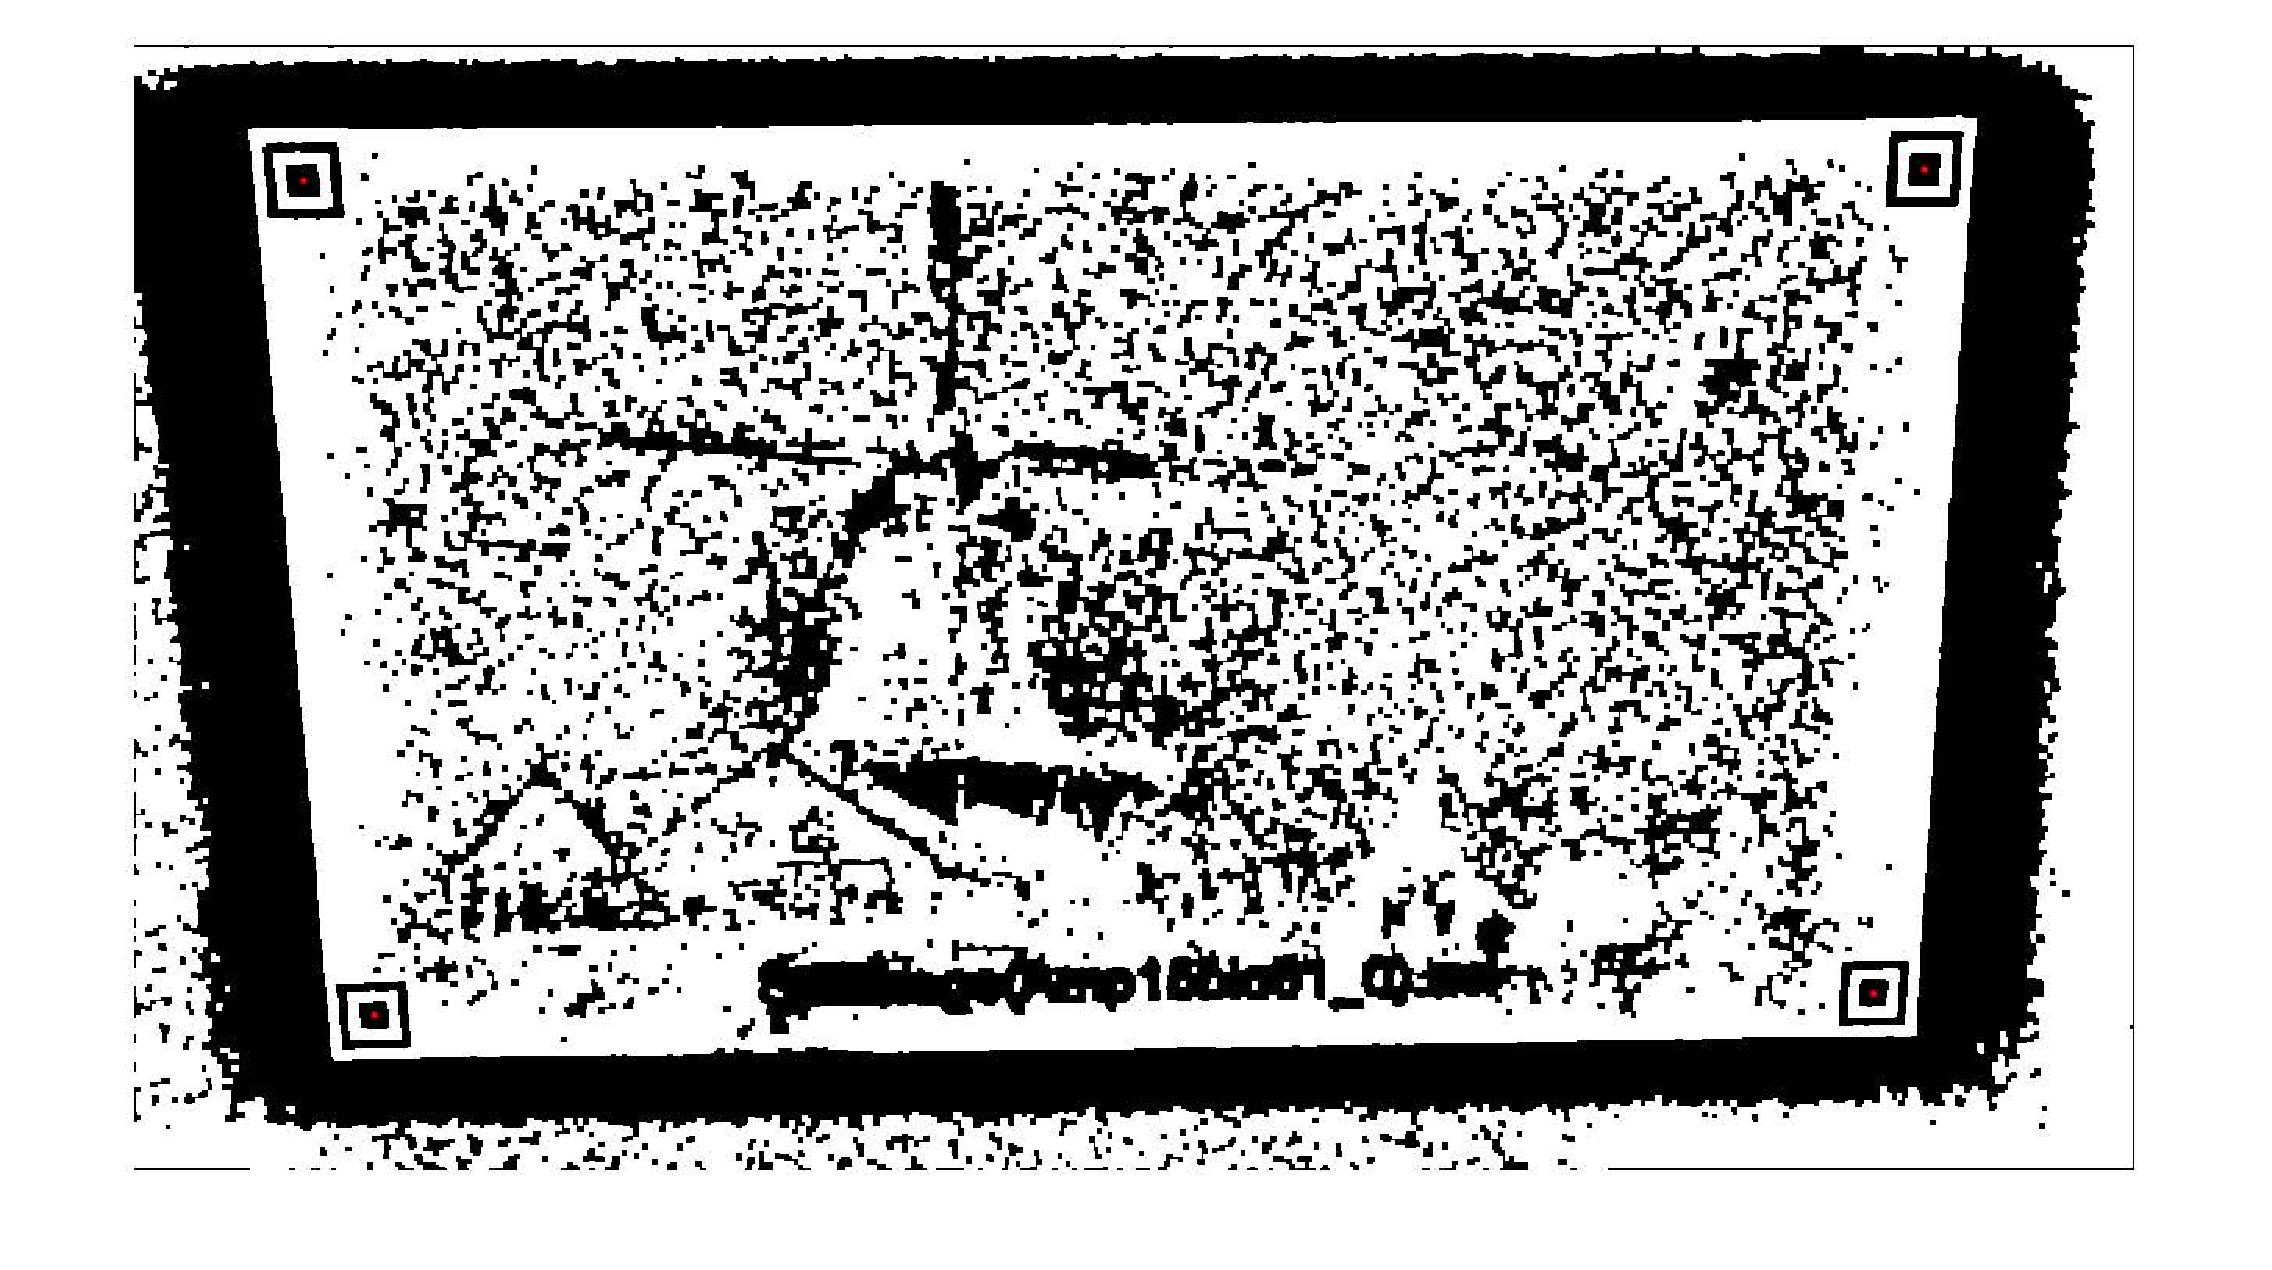
\includegraphics[keepaspectratio,width=1.0\textwidth]{images/3_Ersteverfahren/QRMuster/QR_Patterndetektion.pdf}
 \caption{Beispiel einer QR Muster Detektion}
 \label{fig:QRMusterBeispiel}
\end{figure}
\chapter{Zweite Methode} \label{cha:ZweiteMethode}

In diesem Kapitel werden die erste Erfahrung beschrieben. Zuerst läuft die Vorstellung des DaVid-Systems. Die Systemmodell und Arbeitsprinzip des Systems werden in anschließenden Abschnitt erläutert. Schließlich folgt die mögliche Anwendungsgebiete des Systems.

Nicht vergessen, dass Überschriften nicht aufeinander folgen dürfen\ldots

\section{Allgemeine Struktur}


\section{Binariesierung}

\textbf{Grundlegende globale Schwelle Methode}

Wenn die Histogrammspitzen und -täler des Bildes offensichtlich sind und Doppelpeaks aufweisen, ist die Wirkung dieserMethode besser. Es basiert auf der visuellen Überprüfung des Histogramms und der Schwellenwert wird durch eine iterative Methode erhalten. Die grundlegende Algorithmus ist wie folgt:

1. Wählen eine Paramenter t und einen anfänglichen Schwellenwert $ T_{0} $ aus, wobei der Durchschnitt der maximalen Grauwerte $ l_{max} $ und minimalen Grauwerte  $ l_{max} $ verwendet wird. $ T_{0} = (l_{max}+l_{max})/2 $

2. Segmentieren das Bild mit dem Schwellenwert $ T_{0} $. Dann das Bild besteht aus zwei Teilen: $ G_{1} $ besteht aus die Pixeln mit deren Grauwert größer als $ T_{0} $ und dargegen $ G_{2} $ deren Grauwert kleiner oder gleich als $ T_{0} $.

3. Berechnen den durchschnittlichen Grauwert aller Pixeln in $ u_{1} $ und $ u_{2} $ und den neue Schwellenwert $ T_{1} = (u_{1}+u_{2})/2 $.

4. Falls $ |T_{0} - T_{1}| < t $, dann nehmen $ T_{1} $ als optimalen Schwellenwert. Andernfalls weisen $ T_{1} $ zu $ T_{0} $und wiederholen die Schritte $ 2\sim4 $, bis der optimale Schwellenwert erhalten ist.

\textbf{Grundlegende adaptive Schwellenwert Binarisierungsmethode}

Ein Bildgebungsfaktor ungleichmäßiger Helligkeit bewirkt, dass ein Histogramm, das ansonsten für eine effiziente Segmentierung geeignet wäre, ein Histogramm wird, das nicht effektiv mit einem einzigen globalen Schwellenwert segmentiert werden kann.

Ein Verfahren zur Verarbeitung besteht darin, das Bild weiter in Unterbilder zu unterteilen, um unterschiedliche Unterbilder mit unterschiedlichen Schwellenwerten zu segmentieren. Diese Methode wird als grundlegende adaptive Schwellenwert-Binarisierungsmethode bezeichnet. Das Hauptproblem bei diesem Ansatz besteht darin, das Bild zu unterteilen und den Schwellenwert für das resultierende Teilbild abzuschätzen. Da die Schwelle für jedes Pixel von dem Pixel in der Untergruppe abhängt, die Position im Bild, also solche Schwellen sind adaptiv. 

Ein Verfahren zum Unterteilen von Unterbildern wird für das Bild übernommen. Hier werden drei Arten von Unterteilungsverfahren ausgewählt, und Unterbildermit einer Größe von $ 32\times32,4 \times4,16\times16 $ Pixelwerden jeweils geteilt, und die durchschnittliche Graustufe der Unterbilder wird Sals ein Schwellenwert für die Binärisierung ausgewählt.


\textbf{OTSU adaptive Schwelle Methode}

OTSU\cite{Ostu}, auch bekannt als die maximale Interklassenvarianz, wurde 1979 vom japanischen Gelehrten Otsu vorgeschlagen und ist eine adaptive Schwellenwertbestimmungsmethode, die auch als Otsu bekannt ist.

Die Grundidee des Otsu-Algorithmus ist: Verwenden das Histogramm des Bildes, gemäß der Varianz zwischen dem Vordergrund und dem Hintergrund, um den optimalen Schwellenwert dynamisch zu bestimmen. Setze die Anzahl der Pixeln in einen Bilden ist N, die Graustufe ist $ L(0,1,...,L-1) $. Die Anzahl der Pixeln mit dem Grauswert i ist $ n_{i} $, dann die Wahrscheinlichkeit von i läuft $ P_{i} = \frac{n_{i}}{N} $. Für das Bild stellt das T die Segmentierungsschwellenwert zwischen Vordergrund und des Hintergrund dar. Vordergrund entsprecht die Grauswerte von 0 zu $ T-1 $, dagegen Hintergrund die Grauswerte von T zu $ L -1 $.

Die Wahrscheinlichkeit der Vordergrundgebiet W0 und der durchschnittliche Grauwert U0 sind

\begin{equation}
  w_{0} = \sum_{i=0}^{T-1} p_{i},\quad u_{0} = \sum_{i=0}^{T-1} ip_{i}/w_{0}
\end{equation}

dagegen die Wahrscheinlichkeit der Hintergrundpunkte W1 und der durchschnittliche Grauwert U1 sind

\begin{equation}
  w_{1} = \sum_{i=T}^{L-1} p_{i} = 1-w_{0},\quad u_{1} = \sum_{i=T}^{L-1} ip_{i}/w_{1}
\end{equation}

Dann das gesamte durchschnittliche Grauwert des Bildes ist

\begin{equation}
• u = w_{0}u_{0} + w_{1}u_{1}
\end{equation}

Die Infra-Klassen-Varianz ist definiert als

\begin{equation}
•\sigma^2 = w_{0}(u_{0} - u)^2 + w_{1}(u_{1} - u)^2 = w_{0}w_{1}(u_{0} - u_{1})^2
\end{equation}

Nehmen Schwellenwert T von 0 zu $ L-1 $. Wenn $ sigma^2 $ Maximum ist, wählen der entsprechende T als der optimale Schwellenwert aus.

Die Ostu-Methode verwendet Grauswert Histogramm zur Bestimmen des Schwellenwerts. Es ist eine automatisch non-parametrische Schwellenauswahlmethode. Diese Methode ist einfach zu berechnen, und wird nicht von der Kontrast- und Helligkeitsänderung unter bestimmten Bedingungen beeinflusst und kann das Objekt zufriedenstellend vom Hintergrundbereich trennen.

















\section{Morphologie}

Nach der Binarisierung kann das Bild zahlreiche Unvollkommenheiten erhalten. Insbesondere ist das Binärbild, die durch einfache Schwellenwert erteilt werden, durch Rauschen und Textur verzerrt. 
Die morphologische Bildverarbeitung verfolgt das Ziel, diese Unvollkommenheiten zu beseitigen, indem Form und Struktur des Objekts berücksichtigt werden.

Morphologische Operationen arbeiten auf der Grundlage der Mengenoperation und hängen von der relativen Ordnung des Pixelwerts ab. Diese Eigenschaft macht es besonders geeignet für die Verarbeitung von Binärbildern. Natürlich ist Mengenoperation gleichmäßig gültig für Graustufenbilder. Hier in dieser Arbeit wird es nur in binäre Bilder benutzt. Es erstellt ein neues Binärbild, bei dem das Pixel einen nicht-Null Wert hat, nur wenn der Operation an dieser Position im Eingabebild erfolgreich ist.

Die Eingabedaten für die mathematischen morphologischen Operationen sind zwei Bilder: das zu bearbeitende Bild A und ein Strukturelement B. B ist normalerweise eine kleine Pixelmatrix mit jeweils einem Wert von Null oder Eins. Einige Eigenschaft des Strukturelements werden wie folgend gelegt.

\begin{itemize}

\item Die Matrixdimensionen geben die Größe des Strukturelements an.
\item Das Muster, das aus Einsen und Nullen bestehen, gibt die Form des Strukturelements an.
\item Ein Ursprung des Strukturelements ist üblicherweise eines dessen Pixel, es verlassen sich auch außerhalb des Strukturelements liegen. 

\end{itemize}

Eine übliche Praxis besteht darin, dass ungerade Dimensionen der Pixelmatrix stellen und den Ursprung als das Zentrum der Matrix definieren. Einige grundlegende Strukturelement legt als folgen:

\begin{figure}[htb]
 \centering 
  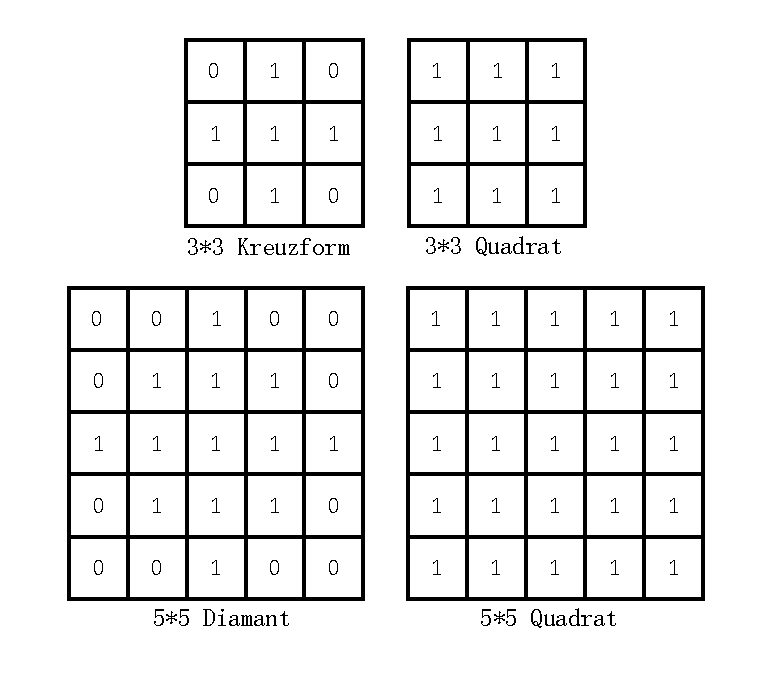
\includegraphics[keepaspectratio,width=0.6\textwidth]{images/4_ZweiteErfahrung/Morphological/strelement.pdf}
 \caption{Einige grundlegende Strukturelement}
 \label{fig:Strukturelement}
\end{figure} 

Als folgend werden zuerst die zwei grundlegende morphologischen Operatoren Erosion und Dilatation beschrieben. Anschließen vorstellen die darauf basierend Operationen, wie als Öffnung und Schließung bekannt sind.

\textbf{Dilatation}

Die Dilatation Operation bewirkt, dass das Objekt nach größer wächst. Das wächst Ausmaß hängt von der Art und Form des Strukturelements ab. Die Formel eine Dilatation wird darstellt als:

\begin{equation}
•A \oplus B =\lbrace z \mid \widehat{(B)_z} \cap A \ne \varnothing \rbrace  
\end{equation}

Hier $ \widehat{(B)_z} $ heißt Strukturelement B um seinen Ursprung reflektiert und um z verschoben. Die entsprechende Dilatation für das Bild A mit B ist die Menge aller Verschiebungen z, die $ \widehat{B} $ und A mindestens ein gemeinsames Element habe. Das Ergebnis der Dilatation läuft, die Pixeln um den Grenze des Objekts hinzufügen. Außerdem die Dilatation Operation wird im wesentlichen verwendet um die Löcher (fehlende Pixel) in einem kontinuierlichen Objekt zu füllen. Es beeinflusst die Intensität an diesem Bereich und kann als ein Unschärfe Effekt beobachtet werden, nämlich eine räumlichen Tiefpassfilter, die beim linearen Filtern des Bildes verwendet werden. Abbildung \ref{fig:Dilatation und Erosion} zeigt eine typische Dilatation Operation.

\begin{figure}[htb]
 \centering 
  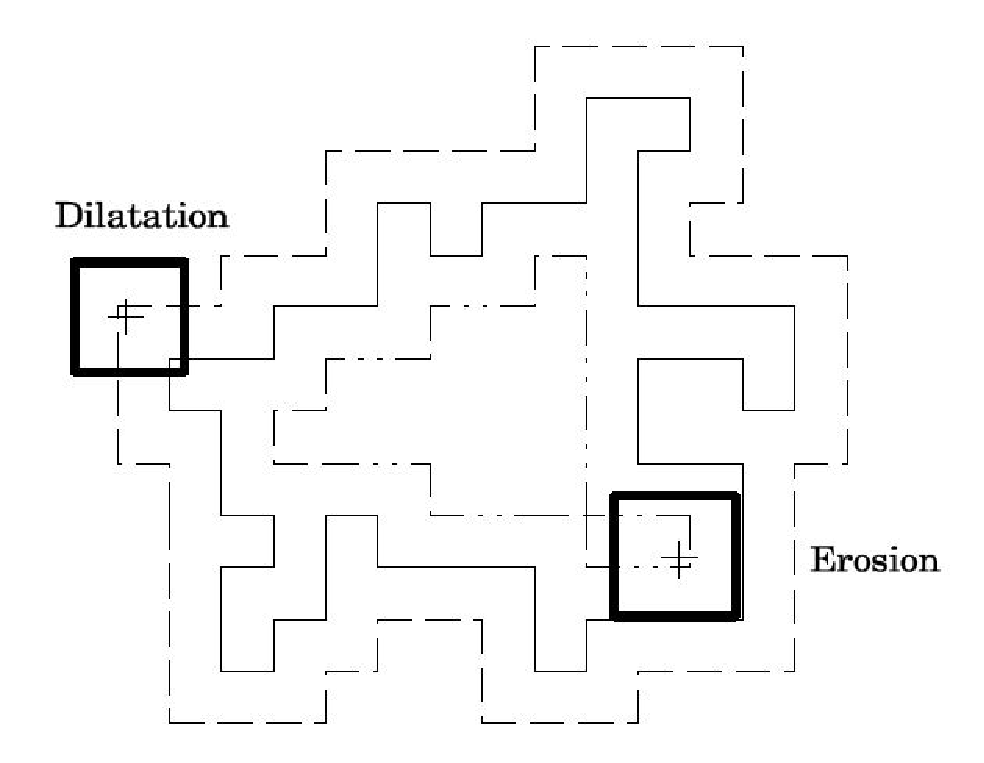
\includegraphics[keepaspectratio,width=0.8\textwidth]{images/4_ZweiteErfahrung/Morphological/DilatationundErosion.pdf}
 \caption{Dilatation und Erosion}
 \label{fig:Dilatation und Erosion}
\end{figure} 


\textbf{Erosion}

Der Operationseffekt eine Erosion ist genau ein Gegenteil von Dilatation. Die Erosion Operation bewirkt, dass das Objekt nach kleiner wechseln. Die Erosion eines Bildes A durch das Strukturelement B ist definiert als 

\begin{equation}
•A \ominus B =\lbrace z \mid (B)_z \subseteq A \rbrace  
\end{equation}

Hier die Erosion des Bilds A ist die Menge aller Punkte z mit derart, dass das Strukturelement B von verschieben wird, zu eine Teilmenge des Bildes A 	gehört. Diese Operation führt zu einem Verlust von Grenzpixeln des Objekts.

Die Erosion Operation entfernt solche Strukturen, die eine kleinere Größe als das strukturierende Element haben. Dann kann es verwenden wird, um die verrauschte "Verbindung" zwischen zwei Objekten zu entfernen. Da die unerwünschten Pixel entfernen werden, ist der Effekt als ein Schärfen des Objekts entsprechen. Als folgend in Abbildung \ref{fig:Dilatation und Erosion} zeigt eine typische Erosion Operation.


\textbf{Öffnung}

Die Öffnung Operation eines Bildes ist eine kombinatorische Operation von Erosion und Dilatation, d.h. zuerst nehmen eine Erosion Operation, danach eine Dilatation Operation. Praktisch werden Bild A durch beide Operationen mit dem gleichen Strukturelement B ausgeführt. Die Formel einer Öffnung Operation ist definiert als

\begin{equation}
•A \circ B =( A \ominus B )\oplus B  
\end{equation}

Die Grenze des geöffneten Objekts sind die Punkte, dass Strukturelement B die äußersten Punkte der Grenze von Objekt erreicht, wenn B innerhalb dieser Grenze entlangfahren. Feine strukturierte Details,
kleiner als das Strukturelement werden demnach beim Öffnung Operation entfernt, dünne Verbindungen zwischen größeren Teilen aufgelöst. Eine Öffnung Operation wird in Abbildung \ref{fig:oeffnungundschliessung} gezeigt.

\begin{figure}[htb]
 \centering 
  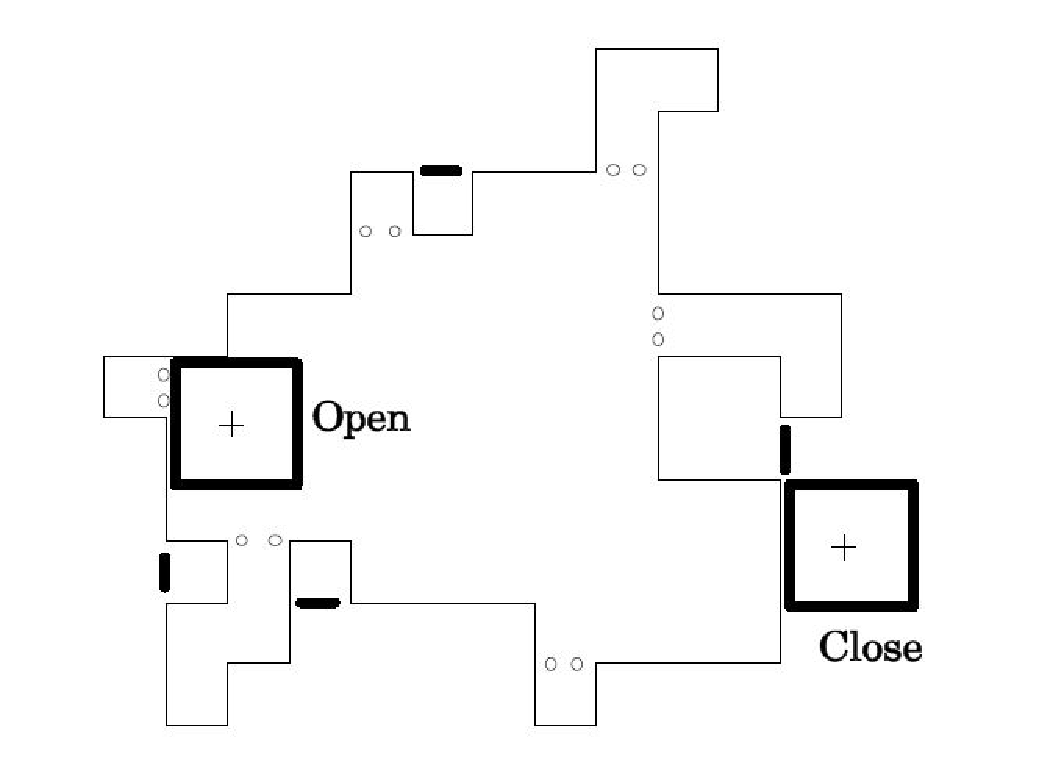
\includegraphics[keepaspectratio,width=0.8\textwidth]{images/4_ZweiteErfahrung/Morphological/oeffnungundschliessung.pdf}
 \caption{Einige grundlegende Strukturelement}
 \label{fig:oeffnungundschliessung}
\end{figure} 

\textbf{Schließung}

Gleichfalls mit Öffnung Operation ist die Schließung Operation auch eine kombinatorische Operation von Erosion und Dilatation. Der Unterschied dazwischen legt der Reihenfolge der Operation, d.h. hier zuerst eine Dilatation Operation, danach eine Erosion Operation mit dem gleichen Strukturelement. Das Schließung eines Bildes A durch das Strukturelement B ist definiert als

\begin{equation}
•A \bullet B =( A \oplus B )\ominus B  
\end{equation}

Die Grenze des geschlossenen Objekts sind die Punkte, dass Strukturelement B, die die äußersten Punkte der Grenze von Objekt erreichen, wenn B außerhalb dieser Grenze entlangfahren. Kleinere Risse, Lücken und feine Details werden dagegen aufgefüllt und mit den großen Teilen zusammengeschlossen. Abbildung \ref{fig:oeffnungundschliessung} zeigt eine Vorgang der Schließung Operation.


Öffnung und Schließung Operation besitzen die folgenden Eigenschaften:

\begin{itemize}

\item Öffnung und Schließung sind idempotent.
\item Die Öffnung Operation ist anti-extensiv. 
\item Die Schließung Operation ist extensiv.
\item Öffnung und Schließung sind dual bezüglich der Komplementierung.
\item Bezeichnet ein Bild als B-Öffnet, wenn es bezüglich gleicher Öffnung Operation unverändert bleibt. 
\item Bezeichnet ein Bild als B-Schließt, wenn es bezüglich gleicher Schließung Operation unverändert bleibt. 

\end{itemize}


\section{Canny detection}

Jetzt können wir ein Binärbild erhalten, das grob in zwei Teile geteilt werden kann, einen Modulationsbereich mit Pixelwert 1 im mittleren und einen umgibt Hintergrundbereich mit Pixelwert 0. Um die nächste Linie Detektion zu implementieren. Machen eine Kanten Detektion, weil Kanten oft mit den Grenzen von Objekten in einer Szene verknüpft werden. Hier ist es die Grenze zwischen Modulationsbereich und Hintergrundbereich. \cite{canny}

Es gibt immer einige gut Kantenextraktionmethod, wie Sobel, Canny, Laplacian, Prewitt, Roberts usw. Hier in dieser Abreit wird die leistungsfähigste Kantenerkennungsmethode bzw. Canny Algorithmus benutzt. Die Canny-Methode unterscheidet sich von den anderen Kantenerkennungsmethoden darin, dass sie zwei verschiedene Schwellenwerte verwendet (um starke und schwache Kanten zu erkennen) und die schwachen Kanten in der Ausgabe nur dann einschließt, wenn sie mit starken Kanten verbunden sind. Diese Methode kann daher im Vergleich zur anderen Method weniger Wahrscheinlichkeit verfügen, durch Rauschen getäuscht zu werden, und mehre Wahrscheinlichkeit verfügen, echte schwache Kanten zu erkennen.

Das Ziel von Canny Algorithmus ist es, einen optimalen Kantenextraktionsalgorithmus zu finden. Drei Kriterien für die optimale Kantendetektion werden vorgeschlagen:

\begin{itemize}

\item Gute Erkennung: Der Algorithmus kann so viele tatsächliche Kanten wie möglich im Bild erkennen.
\item Gute Positionierung: Identifizieren die Kanten so nah wie möglich an den tatsächlichen Kanten im Bild.
\item Minimale Antwort: Kanten in einem Bild können nur einmal identifiziert werden, und mögliches Bildrauschen sollte nicht als Kanten erkannt werden.

\end{itemize}

Die Implemetierung eine Canny Algorithmus läuft:

\begin{enumerate}
	\item \textbf{Gaußsche Unschärfe.} Die Hauptziel ist, Rausch zu entfernen. Da die Rauschen auch auf Hochfrequenzsignale konzentriert ist, wird es leicht als eine falsche Kante erkannt. Anwenden gaußsche Unschärfe, um Rauschen zu entfernen und die Erkennung falscher Kanten zu reduzieren. Es sollte beachtet werden, dass ein zu großer Radius einige schwache Kanten nicht erkennen.
	\item \textbf{Berechnen die Größe und Richtung des Gradienten.} Die Kanten des Bildes können in verschiedene Richtungen zeigen. Daher verwendet der klassische Canny Algorithmus vier Gradientenoperatoren, um die Gradienten in horizontaler, vertikaler und diagonaler Richtung zu berechnen. Jedoch in allgemeine werden diese vier Gradientenoperatoren nicht verwendet, sondern mit Kantenunterschiedsoperatoren (wie Rober, Prewitt, Sobel) die Differenz Gx und Gy in horizontaler und vertikaler Richtung berechnen. Die Berechnung der Gradientengröße und Richtung wie folgt:	
\begin{equation}
\begin{split}
•  G   & = \sqrt{G_x^{2} + G_y^{2}} \\
\theta & = atan2(G_y,G_x)
\end{split}
\end{equation}

Der Gradientenwinkel $ \theta $ liegt im Bereich von Radianten $ -\pi $ bis $ \pi $, dann approximiere es in vier Richtungen, die horizontale, vertikale und zwei diagonale Richtungen repräsentieren    $(0^{\circ}, 45^{\circ}, 90^{\circ}, 135^{\circ}) $. Es kann durch $  \pm i \pi / 8\ (i =1, 3, 5, 7) $ geteilt werden, und der in jedem Bereich fallende Gradientenwinkel einen spezifischen Wert ergibt, der eine von vier Richtungen repräsentieren. Als folgend nehmen eine Beispile mit Sobel Operator.

\begin{equation}
G_x = \begin{bmatrix}
-1 &0 &+1 \\
-2 &0 &+2 \\
-1 &0 &+1
\end{bmatrix} * A \quad and \quad G_y = \begin{bmatrix}
+1 &+2 &+1 \\
0 &0 &0 \\
-1 &-2 &-1
\end{bmatrix} * A
\end{equation}
	
	\item \textbf{Nicht-maximale Unterdrückung.} Nicht-maximale Unterdrückung ist eine Kantenverfeinerungsmethode. Die Gradientenkanten, die normalerweise abgeleitet werden, sind nicht als ein Pixel breit, sonder mehrere Pixel breit. Während Kriterie 3 erfordert, dass die Kante nur eine genaue Punktbreite hat. Nicht-maximale Unterdrückung kann dazu beitragen, den lokalen maximalen Gradienten beizubehalten, während alle anderen Gradientenwerte unterdrückt werden. Dies bedeutet, dass nur die schärfste Position in der Gradientenänderung beibehalten wird. Der Algorithmus ist wie folgt:
	\begin{itemize}
	\item Vergleichen die Gradientenstärke des aktuellen Punkts mit der Gradientenstärke der positiven und negativen Gradientenrichtungspunkte.
	\item Wenn die Gradientenstärke des aktuellen Punktes im Vergleich zur Gradientenstärke anderer Punkte in der gleichen Richtung am größten ist, wird der Wert auf 1 behalten. Ansonsten wird es auf 0 gesetzt. Zum Beispiel, wenn die Gradientenrichtung des aktuellen Punktes in die Richtung von $(90^{\circ}$ direkt darüber zeigt, muss es mit den Pixeln in der vertikalen Richtung direkt darüber und darunter verglichen werden.
	\end{itemize}
	
	Es ist erwähnenswert, dass die positiven und negativen Richtungen keine unterschiedlichen Bedeutungen haben. Zum Beispiel sind die südöstliche Richtung und die nordwestliche Richtung beide als eine Richtung der Diagonalen betrachtet. Vorher approximierten die Gradientenrichtung horizontal, vertikal und zwei Diagonalen in vier Richtungen, so dass jedes Pixel in einer dieser vier Richtungen entsprechend seiner eigenen Gradientenrichtung verglichen wird, um zu bestimmen, ob es beibehalten wird. 
	
	
	\item \textbf{Doppelte Schwelle.} Ein allgemeiner Kantenerkennungsalgorithmus verwendet einen Schwellenwert, um kleine Gradientenwerte entfernen, die durch Rauschen oder Farbänderungen verursacht werden, während große Gradientenwerte beibehalten werden.
Der Canny Algorithmus wendet einen doppelten Schwellenwert, d.h. einen hohen Schwellenwert und einen niedrigen Schwellenwert an, um Kantenpixel zu unterscheiden. Wenn der Kantenpixelpunktgradientwert größer als den hohen Schwellenwert ist, wird er als einen starken Kantenpunkt betrachtet.	Wenn der Kantengradientenwert kleiner als der hohen Schwellenwert und größer als den niedrigen Schwellenwert ist, wird er als einen schwachen Kantenpunkt markiert. Punkte, die unterhalb der niedrigen Schwelle, werden unterdrückt.

	\item \textbf{Hysterese Grenzenverfolgung.} Bisher können die starke Kantenpunkt als echte Kanten angesehen werden. Dagegen die Schwache Kantenpunkte können echte Kanten sein, jedoch sie können auch durch Rauschen oder Farbänderungen verursacht sein. Um genaue Ergebnisse zu erhalten, sollten die zweite Möglichkeit von schwachen Kantenpunkte entfernt werden. In allgemein werden die schwache Kantenpunkte und die starke Kantenpunkte, die durch reale Kanten verursacht werden, als verbunden betrachtet, während die schwache durch Rauschen verursacht Kantenpunkte, dies nicht verbunden sind. Der sogenannte Hysterese Grenzenverfolgung Algorithmus untersucht die achte verbundene Pixel eines schwachen Kantenpunktes, solange ein starker Randpunkt vorhanden ist, wird dieser schwache Randpunkt als echt Kantenpunkte betrachtet und die Wert als 1 bleibt.
	
Zur Implementierung dieser Schritt sucht nach allen verbundenen schwachen Kanten. Wenn ein Punkt einer verbundenen schwachen Kante mit einem starken Kantenpunkt verbunden ist, wird die schwache Kante beibehalten, snsonsten unterdrücken diese schwache Kante. Bei der Suche kann der Algorithmus "Breite zuerst" oder "Tiefe zuerst" verwenden. Nachdem der gesamten Suche des Bildes, werden die Nicht-Kantenpunkte entfernt, d.h. der Wert  auf 0 gesetzt wird.
	
\end{enumerate}

Abbildung \ref{fig:canny} zeigt ein Ergibnis mit Canny Kantenextraktion.

\begin{figure}[H]
 \centering 
  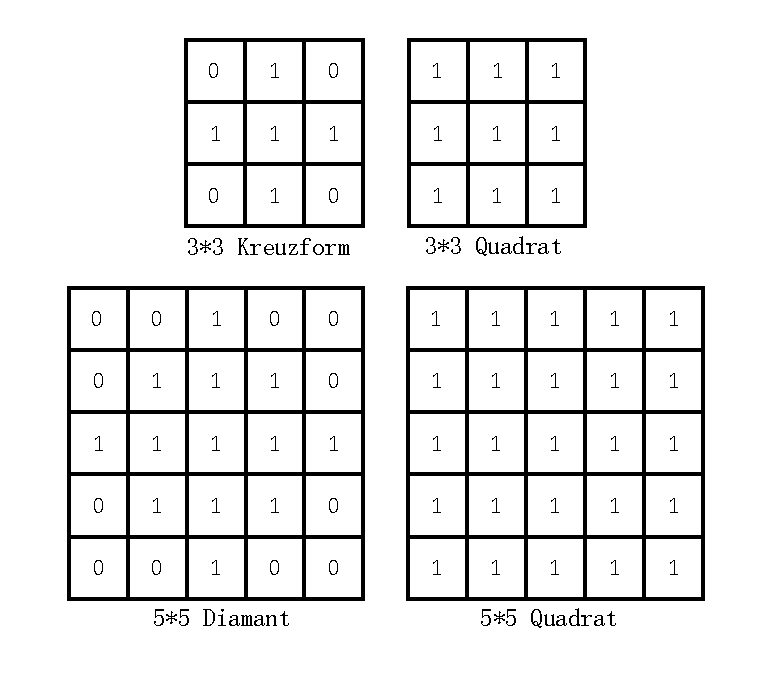
\includegraphics[keepaspectratio,width=0.4\textwidth]{images/4_ZweiteErfahrung/Canny/canny.pdf}
 \caption{Einige grundlegende Strukturelement}
 \label{fig:canny}
\end{figure} 

\section{Hough detection}





\chapter{Auswertung} \label{cha:Auswertung}

Text hier zwischen. Referenz auf ein Bild mit cleverref (siehe \cref{fig:mathplot}). Und dann noch ein paar Zitierungen \cite{Reinhold:2013fk,Moon,IEEE2011}.

\section{Section}

Jetzt nur noch schreiben! :)



\chapter{Zusammenfassung} \label{cha:Zusammenfassung}

In dieser Arbeit werden zwei Verfahren zur Ausschnittsdetektion für die Screen-Camera Visible Light Communication untersucht und implementiert. Methode 1 ist vom differentiellen Modulationsverfahren des David-Systems inspiriert. d.h. Daten werden mit geringer Amplitude im Videosignal differentiell überlagert. In der Methode wird ein QR Muster an jeder Ecke der Datenebene hinzugefügt und dann mit den Daten zusammen hinter dem Bild moduliert. Diese Methode kann nicht nur den unschönen Effekt lösen, welcher durch direktes Hinzufügen des QR Musters zu dem Videobild verursacht wird, sondern kann auch den QR Muster durch seine spezifische geometrische Eigenschaft, d.h. in jeder Richtung beträgt das Breiteverhältnis $1:1:3:1:1$, effektiv erkennen. Dadurch wird schließlich der Modulationsbereich bestimmt. Das 2. Verfahren wird in den physikalischen Eigenschaften des Modulationsbereichs ausgeführt. Im \gls{david} System wirkt der Bildschirm als Übertragungsende, und der Bildschirmbereich ist der Modulationsbereich, der im Allgemeinen in Form eines Rechtecks ist. Dadurch kann dieses Problem in eine rechteckige Erkennung umgewandelt werden. Durch die Radon Transformation wird die längste gerade Linie in dem Bild detektiert, um ein Rechteck bzw. den Modulationsbereich, zu bestimmen.

zwei Aufnahmebedingungen wurden in dieser Arbeit berücksichtigt, eine ist die Aufnahme mit dem Smartphone aus der Hand und die andere auf einem Stativ. Handheld-Kamera-Shooting ist eine der häufigsten und bequemsten Aufnahmemethoden im Alltag, und hat eine unerlässliche Position in der praktischen Anwendung. Zu diesem Zweck wurde ein Bildregistrierungsmodul speziell für Handschütteln entwickelt, welche Merkmals Detektion, \gls{ransac}, Kamera Modell und Nichtlineare Optimierung beinhaltet. Beim Testen beträgt die relative Verschiebung zwischen den entsprechenden Punkten des korrigierten Bildes c.a. 0.3 Pixel. Dies führt zu einem relativ guten Differenzbild. Dieser spielte eine wichtige Rolle weil beide Verfahren in dieser Arbeit auf der Detektion von Differenzbildern basieren. Dafür wird der Begriff $ ``Energie" $ eingeführt, welcher die Klarheit des Modulationsbereichs repräsentiert. Gemäß der Energiesortierung werden die klarsten Bilder ausgewählt und hinzugefügt, um das zu detektierende Bild zu erhalten. In Methode 1 werden die beide obigen Schritte implementiert, und durch Auswertung die durchschnittliche Abweichung ca. $ 1-2 $ Pixel bemessen. Es sollte hier angemerkt werden, dass aufgrund der Eigenschaften der Bildregistrierung das Video, das in Methode 1 aufgenommen wurde, ein statisches Video ist, d.h. der Inhalt des Videos hat sich nicht geändert. Der Grund dafür ist, dass der Punkt der Merkmals Detektion hauptsächlich auf dem Inhalt des Videos basiert. Wenn sich der Videoinhalt stark ändert, ist es schwierig, die Genauigkeit der Bildwiederherstellung zu garantieren. Einige bei der Arbeit versuchten Methoden war die Abschirmung des zentralen Bereichs während der Merkmals Detektion, d.h. nur die Merkmale in der Umgebung des Bildes wurden erkannt, was nicht zufriedenstellend ist. Methode 2 implementiert die Erkennung des Modulationsbereichs unter Verwendung eines Stativs. Nach der Erkennung beträgt die durchschnittliche Abweichung ebenfalls ca. $ 1-2 $ Pixel. In beiden Methoden kann der Modulationsbereich mit Parametern, wie die Modulationsapmlitude als 4,  der Datenblock als $ 4 \times 4 Pixel$, erfolgreich bestimmt werden. 

Für dieses Thema gibt es einige mögliche weitere Forschung in der Zukunft. Zuerst kann wie oben erwähnt, ein Verfahren gefunden werden, welches beim Aufnehmen des dynamischen Videos mit dem Smartphone aus der Hand, das Handschütteln-Problem effektiv löst. Der Fokus liegt darauf, die Wirkung vom Video-Inhalt zu neutralisieren und das Bild nur auf die Merkmale des Hintergrunds zu filtern. Zweitens, die in dieser Arbeit verwendete Differenzbild Optimierungsmethode, kann aufgrund der Berechnung der $ ``Energie" $ für jedes Differenzbild zu einer großen Rechenlast führen. Ein effektives Verfahren wäre versuchen, ein zu detektierendes Bild, das auf dem bekannten Differenzbild basiert, effizient zu generieren. Schließlich wurde in Experiment festgestellt, dass unter denselben Parametern die Verwendung des gleichen Smartphones mit dem gleichen Video-Inhalt auf verschiedenen Bildschirmen, zu unterschiedlichen Ergebnissen führt. Dadurch können die Auswirkungen der Bildschirmfaktoren, wie z.B. Beleuchtungsart, Auflösung, Bildwiederholfrequenz, weiter erforscht werden.






\appendix
\chapter{Erster Anhang} \label{cha:anhangA}

\section{Section}

Jetzt nur noch schreiben! :)




\backmatter
\cleardoublepage
% \chapter*{Nomenklatur} \addcontentsline{toc}{chapter}{Nomenklatur}
% \markboth{Nomenklatur}{Nomenklatur}

\printglossary[type=\acronymtype, style=tab_style] %[toctitle=Symbolverzeichnis,title=Symbolverzeichnis] 
\printglossary[type=symbol, style=tab_style_sym]
% \printglossary

\listoffigures%				Abbildungsverzeichnis
\listoftables%				Tabellenverzeichnis
\lstlistoflistings%			Listingsverzeichnis

% \nocite{*}%				es wird alles zitiert
\printbibliography%			Literaturverzeichnis

\makeatletter
\cleardoublepage
\thispagestyle{empty}
\onehalfspacing
\LARGE
\begin{center}
	\textbf{Eidesstattliche Versicherung}
\end{center}

\small
\vspace{\baselineskip}
\underline{\makebox[.4\textwidth][c]{\@authorsurname,\space\@authorfirstname}}
\hspace{.25\textwidth}
\underline{\makebox[.3\textwidth][c]{\@matrikelnumber}}
\newline
\makebox[.4\textwidth][l]{Name, Vorname}
\hspace{.25\textwidth}
\makebox[.3\textwidth][l]{Matr.-Nr.}

Ich versichere hiermit an Eides statt, dass ich die vorliegende \@documenttype\space mit dem Titel

\underline{\makebox[0.97\textwidth][c]{\@thesistitle}}

selbstständig und ohne unzulässige fremde Hilfe erbracht habe. Ich habe keine anderen als die 
angegebenen Quellen und Hilfsmittel benutzt sowie wörtliche und sinngemäße Zitate kenntlich 
gemacht. Die Arbeit hat in gleicher oder ähnlicher Form noch keiner Prü\-fungs\-be\-hörde 
vorgelegen. 
\vspace{\baselineskip}

\underline{\makebox[.4\textwidth][c]{Dortmund, \today}}
\hspace{.25\textwidth}
\underline{\hspace{.3\textwidth}}
\newline
\makebox[.4\textwidth][l]{Ort, Datum}
\hspace{.25\textwidth}
\makebox[.3\textwidth][l]{Unterschrift}

\vspace{\baselineskip}

\textbf{Belehrung}: 

Wer vorsätzlich gegen eine die Täuschung über Prüfungsleistungen betreffende Regelung einer 
Hochschulprüfungsordnung verstößt, handelt ordnungswidrig. Die Ordnungswidrigkeit kann mit 
einer Geldbuße von bis zu 50.000,00\,€ geahndet werden. Zuständige Verwaltungs\-behörde für 
die Verfolgung und Ahndung von Ordnungswidrigkeiten ist der Kanzler/die Kanzlerin der 
Technischen Universität Dortmund. Im Falle eines mehrfachen oder sonstigen schwerwiegenden 
Täuschungs\-versuches kann der Prüfling zudem exmatrikuliert werden. (§ 63 Abs. 5 
Hochschulgesetz - HG - )  

Die Abgabe einer falschen Versicherung an Eides statt wird mit Freiheitsstrafe bis zu 3 Jahren 
oder mit Geldstrafe bestraft.  

Die Technische Universität Dortmund wird ggf. elektronische Vergleichswerkzeuge (wie z.B. die 
Software „turnitin“) zur Überprüfung von Ordnungswidrigkeiten in Prüfungsverfahren nutzen. 

Die oben stehende Belehrung habe ich zur Kenntnis genommen: 
\vspace{\baselineskip}

\underline{\makebox[.4\textwidth][c]{Dortmund, \today}}
\hspace{.25\textwidth}
\underline{\hspace{.3\textwidth}}
\newline
\makebox[.4\textwidth][l]{Ort, Datum}
\hspace{.25\textwidth}
\makebox[.3\textwidth][l]{Unterschrift}
\makeatother
\end{document}